%!TEX program = xelatex
\documentclass [PhD] {uclathes}
\usepackage[toc,page]{appendix}
\usepackage[noprefix]{nomencl}
\usepackage{lscape}
\makeglossary \makeindex
\usepackage[table]{xcolor}
\usepackage{amsmath}
\usepackage{placeins}
\usepackage{amsbsy}
\usepackage{color}
\usepackage[superscript,biblabel]{cite}
\usepackage{amssymb}
\usepackage{longtable}
\usepackage{verbatim}
\usepackage{chngpage}
 \ifx\pdfoutput\undefined
   \usepackage[dvips]{graphicx}
   \else
   \usepackage[pdftex]{graphicx}
   \pdfcompresslevel=9
   \fi
\usepackage{array}
\usepackage{float}
\usepackage[colorlinks,citecolor=red,linkcolor=blue]{hyperref}
\usepackage{subfiles}
\usepackage{xltxtra} % Extra customizations for XeLaTeX
\usepackage{tabularx, multirow, booktabs}
\newcommand{\otoprule}{\midrule[\heavyrulewidth]}
\usepackage{subcaption}
\usepackage{siunitx}
\usepackage{textcomp}%it was suggested online to load this before gensymb to get rid of an annoying error
\usepackage{gensymb}
\setcounter{secnumdepth}{5}
\setcounter{tocdepth}{2}
%\linespread{1.6}%double line (1.6%) spacing, for one & half use {1.3}
\usepackage{cleveref}
% \usepackage[version=3]{mhchem}
% \usepackage{chemmacros}
%vanlew-environments

% time derivative
\newcommand{\dt}[1]{
\frac{\mathrm{d}{#1}}{\mathrm{d}t}}
\newcommand{\ddt}[1]{
\frac{\mathrm{d}^2{#1}}{\mathrm{d}t^2}}

% partial derivative (with optional numerator and required denominator)
\newcommand{\pder}[2][]{\frac{\partial#1}{\partial#2}}

% custom vector notation
\renewcommand{\vec}[1]{\mathbf{#1}}



\newcommand{\lit}{Li$_2$TiO$_3$~}
\newcommand{\lis}{Li$_4$SiO$_4$~}
\sisetup{locale = US}


% Dimensionless numbers
\newcommand{\Nu}{\mathrm{Nu}}
\renewcommand{\Re}{\mathrm{Re}}
\renewcommand{\Pr}{\mathrm{Pr}}
\newcommand{\Ra}{\mathrm{Ra}}
\newcommand{\Bi}{\mathrm{Bi}}
\newcommand{\Fo}{\mathrm{Fo}}








                        % personal LaTeX macros


\title          {Shitty Dissertation Title}
\author         {Jon Thomas Van Lew}
\department     {Mechanical Engineering}
\degreeyear     {2015}

\chair{Mohamed Abdou}
\member{Alice Ying}
\member{Pirouz Kavehpour}
\member{Nasr Ghoniem}
\member{Jaime Marian}

%\dedication     {\textsl{To My loved ones \ldots without \\
%                whom I could not find the will\\
%      and courage to do this}}

\acknowledgments {I did it all on my own}

\vitaitem {2005} {B.S., Mechanical Engineering, Cum Laude\\ University of Arizona\\ Tucson, AZ}
\vitaitem {2010} {M.S., Mechanical Engineering \\ University of Arizona \\ Tucson, AZ}

\abstract{It's all crap}

\begin{document}

%%%%%%%%%%%%%%%%%%%%%%%%%%%%%%%%%%%%%%%%%%%%%%%%%%%%%%%%%%%%%%%%%%%%%%%%%
%\makeintropages

%\mymaketitlepages              % Thesis Title Page
%\mymakecopyrightpage           % Copyright Page
%\pagenumbering{roman}
%\setcounter{page}{1}
%\mymakeabstractpage            % Abstract Page
%\mymakesignaturepage           % Committee Member Signature Page
%\setcounter{page}{4}
\tableofcontents               % Table of Contents
%\listoffigures                 % List of Figures
%\listoftables                  % List of Tables
%\chapter*{Nomenclature}

\begin{tabbing}
aaaaaaaaa\= aaaaaaaaa\kill
$A$ \>        sample cross-sectional area, m$^2$\\
$A_s$ \>        sample surface area, m$^2$\\
$b$ \>        sample thickness, m \\
$Bi$ \>       Biot number (=$hb/k$) \\
$c_p$ \>      specific heat, J/kg$\cdot$K\\
$C$ \>        capacitance, F \\
$D$ \>        electric displacement, C/m$^2$\\
$d_{33}$ \>   piezoelectric coefficient, C/N\\
$\Delta h$ \>  specific phase change enthalpy, J/kg\\
$E$ \>        electric field, V/m\\
$E_{br}$ \>    electrical breakdown field, V/m\\
$E_{c}$ \>    coercive electric field, V/m\\
$f$ \>        frequency, Hz\\
$g$ \>          gravity of Earth (=9.81 m/s$^2$) \\
$h$    \>     heat transfer coefficient, W/m$^{2}$$\cdot$K \\
$k$ \>        thermal conductivity, W/m$\cdot$K\\
$I_p$ \>      electric current, A\\
M$_A$ \>       monoclinic M$_A$ crystal phase \\
M$_B$ \>       monoclinic M$_B$ crystal phase \\
M$_C$ \>       monoclinic M$_C$ crystal phase \\
$mol\%$\>    molar fraction, \% \\
MPB \>         morphotropic phase boundary \\
$N_D$ \>      energy density, J/L\\
$Nu$ \>     Nusselt number \\
O \>       orthorhombic crystal phase \\
$p_c$ \>      pyroelectric coefficient, C/m$^2$$\cdot$K\\
$P$ \>        polarization density, C/m$^2$\\
$P_D$ \>      power density, W/L\\
$P_r$ \> 	  remnant polarization, C/m$^2$\\
$P_s$ \> 	  saturation polarization, C/m$^2$\\
$Q$ \> 	      charge, C \\
$Q_{in}$ \>     thermal energy input per unit volume, J/m$^3$ \\
PE \> 	  pyroelectric element \\
R \>       rhombohedral crystal phase \\
$R$ \> 	      resistance, $\Omega$ \\
$Ra$ \>         Rayleigh number \\
$S$ \>          side length, m \\
$s_{33}$ \>   elastic compliance, m$^{2}$/N \\
$t$ \>        time, s\\
T \>       tetragonal crystal phase \\
$T$ \>        temperature, $^o$C or K\\
$T_{Curie}$ \> Curie temperature, $^o$C\\
$x$ \>	      molar fraction of lead titanate, \%\\
$x_{3}$ \>	  strain in longitudinal direction [=$\int_{T_{C}}^{T} \! \alpha(T) \, \mathrm{d} T$] \\
$-\!\!\!\! V$ \>      volume, m$^3$ \\
$V$\>         voltage, V \\
$V_{1}$\>     voltage across capacitor, V \\
$V_{2}$\>     voltage across resistor, V \\
$W_{in}$ \>     mechanical energy input per unit volume, J/m$^3$ \\
\\

\textbf{Greek symbols} \\
$\alpha$ \>     linear thermal expansion coefficient, K$^{-1}$\\
$\delta$  \>    relative error between experimental data and model predictions, \% \\
$\varepsilon_{o}$  \> vacuum permittivity (= 8.854x10$^{-12}$ F/m) \\
$\varepsilon_{r}$ \>  relative permittivity  \\
$\eta$ \>          material efficiency, \% \\
$\nu$ \>        kinematic viscosity, m$^2$/s \\
$\rho$     \>     density, kg/m$^3$ \\
$\sigma$   \>     elastic stress, Pa \\
$\tau$$_{t}$     \>   thermal characteristic time constant, s\\
$\tau_{ij}$ \>   duration of process $i$-$j$, s\\
\\

\textbf{Subscripts} \\
$avg$ \>  refers to average \\
$b$ \>      refers to bias \\
$cold$ \>  refers to cold \\
$eff$ \>   refers to effective \\
$f$ \>      refers to fluid \\
$H$ \>    refers to high \\
$hot$ \>   refers to hot \\
$L$ \>    refers to low \\
$max$  \>   refers to maximum \\
$PE$ \>    refers to pyroelectric element \\
\end{tabbing}





%\printglossary                 % Nomenclature Page
%\mymakeacknowledgmentspage     % Acknowledgments Page
%\mymakevitapages               % Vita Page
%\mytitlefinish                 % Start a New Page for Chapter 1.

%%%%%%%%%%%%%%%%%%%%%%%%%%%%%%%%%%%%%%%%%%%%%%%%%%%%%%%%%%%%%%%%%%%%%%%%%%%
%\pagenumbering{arabic}
%\setcounter{page}{1}

% Reference sections
%%%%%%%%%%%%%%%%%%%%%%%%%%%%%%%%%%%%%%%%%%
\chapter{Introduction} \label{sec:introduction}
%%%%%%%%%%%%%%%%%%%%%%%%%%%%%%%%%%%%%%%%%%
The controlled, sustained thermonuclear fusion of light elements is the ultimate energy source; it is inexhaustible (on our planetary scales), produces none of the greenhouse gases that are altering the climate, and avoids many of the dangers of nuclear fission. Overcoming the engineering obstacles to tame the fusion reaction is the greatest technological challenge of our generation. A recently-published book by Dr. Francis Chen provides an excellent coverage of the basics of fusion energy, the reactions, our present understanding of the fusion plasma, and the role fusion energy can play in the global energy market.\cite{Chen2011} 

In this dissertation, I will begin by presenting only an extremely brief summary of the main points on the background of general fusion technology as necessary for establishing a common language that will be used in the rest of the document. Slightly more background will be given for the fusion nuclear technology that are immediately relevant to the research I have performed, specifically the breeder blanket of a fusion reactor.

\section{The Basics of Nuclear Fusion and Tritium Breeding}\label{sec:fusion-basics}

The fusion reaction assumed to be the first choice demonstrable fusion power plants involves the two hydrogen isotopes of deuterium and tritium. The deuterium-tritium (DT) reaction has a high reaction probability at the lowest ion temperature and a high energy yield. Alternative fusion reactions of two deuterium atoms or a deuterium atom with helium-3 are advantageous in other regards, such as no radioactive byproducts or fuel availability, but their relatively-higher ion temperature preclude them from current consideration.\cite{abdou} The DT reaction proceeds as
\begin{align}
	\mathrm{D} + \mathrm{T}&\xrightarrow{}\ ^4\mathrm{He}+\mathrm{n}+17.58\ \text{MeV} \label{eq:dt-reaction}
\end{align}

Of the two isotopes fused, deuterium ($D$, or $^2$H) is a stable isotope and is naturally occurring in an average abundance of 0.015 mole percent in water on Earth. To demonstrate just how plentiful deuterium is as a fuel source, there is approximately 100 million billion kilograms of deuterium in the Earth's oceans. If all energy on Earth were produced from DT fusion power plants, there would be enough deuterium to outlast the lifetime of our sun. It is safe to say we will not exhaust our deuterium sources on Earth.

Tritium ($T$, or $^3$H), however, is radioactive with a half-life of only about 12.32 years; any naturally occurring tritium decays at such a rapid pace it will never accumulate to an appreciable amount on Earth. If tritium is to be used as a fuel in a fusion power plant, it must be generated artificially -- thus the need for the so-called tritium breeding blankets in fusion reactors. In-situ generation of tritium in a fusion reactor is possible with the assistance of lithium. Natural lithium will interact with neutrons as
\begin{subequations}\label{eq:lithium-t}
\begin{align}
	\mathrm{n} + \ ^7\mathrm{Li} &\xrightarrow \ \mathrm{n}+\alpha + \mathrm{T} -2.47\ \text{MeV}\label{eq:li7-t}\\
	\mathrm{n} + \ ^6\mathrm{Li} &\xrightarrow \  \alpha + \mathrm{T} +4.78\ \text{MeV} \label{eq:li6-t}
\end{align}
\end{subequations}
where we have used the common short-hand of $\alpha$ in place of the helium nucleus. The cross-sections of the lithium reactions are given in Fig.~\ref{fig:li-xsects}. Note the exothermic lithium-6 reaction (a neutron of any energy will incite the transmutation) and the threshold energy required of the incident neutron in the endothermic lithium-7 reaction. The exothermic reaction is also the source of energy that will ultimately generate the electricity of the fusion power plant.

\begin{figure}[ht]
	\centering
	\includegraphics[width=0.6\textwidth]{chapters/figures/breeding_xsecs} 
	\caption{Cross-sections of various blanket materials. Note the threshold for the $^7$Li and neutron multiplying reactions.}
	\label{fig:li-xsects}
\end{figure}

Lithium, like deuterium, is quite abundant on Earth. To make the point clear, there is enough lithium accessible in the Earth's crust to generate tritium for 30 million years worth of DT reactions if they were providing all of humanity's electricity.\cite{Chen2011}. Thus lithium is an excellent candidate for generating the tritium necessary to self-sustain the fusion reaction in a power plant. Lithium is the main material component of tritium breeder blankets -- the form of lithium as it exists in the breeding blanket is a source of continued research.

At present there are two main avenues of tritium breeder designs: those containing liquid or solid lithium. Many of the functional requirements are similar between the two designs but their implementation is quite different. While much research has been -- and continues to be -- performed on the liquid breeder design (for examples, see Refs.~[cite many liquid breeder papers]), the work of this dissertation focuses solely on a particular solid breeder design. In the next section I will refer to the breeding blanket almost exclusively as the ``solid breeder'' though it should be understood that many of the generic features and requirements of the solid breeder are shared with its sister design, the liquid breeder.

\subsection{Breeding Blanket for Fusion Reactors}


\begin{figure}[ht]
	\centering
	\includegraphics[width=1\textwidth]{chapters/figures/demo} 
	\caption{An example design of a DEMO reactor with solid breeder blankets shown as inboard (IB) and outboard (OB) blanket components.}
	\label{fig:demo}
\end{figure}

\begin{figure}[ht]
	\centering
	\includegraphics[width=0.85\textwidth]{chapters/figures/solid_breeder_sketch} 
	\caption{Sketch of a typical unit of a pebble bed tritium breeding zone. The pebble bed is cooled with contact to the containing structure.}
	\label{fig:solid-breeder-sketch}
\end{figure}

The breeder blanket is a pivotal piece of engineering technology upon which the success of a fusion power plant rests. The successful operation of a breeder will see the device capture the neutrons ejected from the fusion reaction to generate fuel for future reactions, breed and recover fuel for the fusion reaction, act as shield to other sensitive equipment, and convert energy into extractable heat for electricity production. Figure~\ref{fig:demo} shows an example sketch of a demonstration (DEMO) fusion reactor and the relative location of the breeder blanket modules as they face the plasma in the torus of the tokamak. 

From the inception of the solid breeder concept in 1975 by Abdou\etal\cite{Abdou1975c}, designs have evolved significantly to meet the requirements of operation in the harsh fusion environment. Currently, the reference solid breeder design incorporates packed beds of ceramic pebbles (spherical particles) that are filled into containment structures of sizes optimized for thermophysical and tritium responses. The main features of many reference designs is illustrated in the sketch of Fig.~\ref{fig:solid-breeder-sketch}.

The pebble bed of Fig.~\ref{fig:solid-breeder-sketch} is contained by a low-activation steel which serves as both mechanical and thermal boundaries for the ensemble. The breeding blanket will experience high volumetric heating (resulting from secondary $\gamma$ rays and the kinetic energy of neutrons that are carrying away approximately 80\% of the fusion reaction) and temperatures will be allowed to increase to approximately 900~\celsius. The heat is conducted via the purge gas and inter-particle contacts between pebbles to the structural material. A high pressure (approximately 8 MPa) helium coolant is then run through the structure. The coolant will heat to approximately 500~\celsius before exiting the blanket, maintaining the structure below structural temperature limits. The heat carried away by the coolant ultimately works its way into an electricity-producing cycle. 

As the neutrons bombard the lithiated ceramic, tritium is produced internal to the pebbles. The tritium atoms work their way slowly to the surface of the pebble whereupon they desorb into a passing, low-pressure (approximately atmospheric) helium purge gas. Tritium that transmutes from the lithium inside the pebble will diffuse slowly through the bulk until reaching a grain boundary. Tritium moves relatively quickly along the grain boundary until reaching a surface of open porosity where it may desorb into the passing purge gas.\cite{Federici1990} The low-speed purge gas is pumped through the pebble bed to extract the tritium generated and transport it out of the blanket for processing. 

The dual role of the breeding blanket to generate heat and tritium forces a specific operational temperature window for the ceramic pebble beds. The low end of the temperature window is governed by a minimum temperature for acceptable release rates of tritium from the ceramic to the purge gas; the value is generally set around 300~\celsius. The upper limit of the temperature window is chosen to avoid sintering of the lithiated ceramic, giving the approximately 900~\celsius limit. Based on current understanding of tritium release from the pebble, as grains grow during sintering of the ceramics the tritium release rate is expected to decrease.

\begin{figure}
        \centering
        \begin{subfigure}[b]{\doubleimagewidth}
                \includegraphics[width=\textwidth]{chapters/figures/keff-pressure}
                \caption{Effective conductivity of ceramic pebble beds is dependent on the pressure of the interstitial gas, a minimum of about $k_\text{eff} = 1$~W/m-K in vacuum.}
                \label{fig:keff-pressure}
        \end{subfigure}%
        
          %add desired spacing between images, e. g. ~, \quad, \qquad, \hfill etc.
          %(or a blank line to force the subfigure onto a new line)
        \begin{subfigure}[b]{\doubleimagewidth 	}
                \includegraphics[width=\textwidth]{chapters/figures/lit-keff-exp}
                \caption{The effective conductivity of pebble beds is weakly dependent on external mechanical pressure and is always approximately $k_\text{eff} = 1$~W/m-K in helium.}
                \label{fig:keff-lit}
        \end{subfigure}
        \caption{Effective conductivity of lithium ceramics.}\label{fig:keff}
\end{figure}

The size of breeder region is limited by the operational temperature window that must be held in spite of the the poor effective conductivity of packed beds of ceramic pebbles. The conductivity is experimentally shown to be a weak function of external pressure but can generally no greater than about \si{1 W/{mK}} -- for well-packed beds. Because the effective conductivity and packed bed-wall interface conductance is predominately a contact conduction, disruptions to the packing structure will have considerable impact on the heat transfer of the packed bed.

Moreover, as nuclear energy is deposited into the poorly-conductive ceramic breeder material and the temperature climbs well above the containing structure, it will confine the thermal expansion of the lithium ceramic and lead to mechanical stresses at the points of contact of the individual pebbles in the packed bed. Engineering design issues surrounding this thermally-induced stress is of great concern to researchers and will be the focus of much of this report.





 % the fusion reaction deposits   The nuclear heat generated in the pebble bed solid breeder will heat the ceramic pebbles to maximum temperatures of approximately 900~\celsius. The heat of the pebbles is transported through them via conduction through inter-particle contacts, conduction through the purge gas into neighboring particles, and ultimately through contact with the containing structure. The box structure surrounding the solid breeder will have high pressure (\si{8~MPa} in many current designs) 


























\section{Motivation}\label{sec:motivation}
\subsection{Pebble Bed Integrity, Thermophysics, and the Role of Modeling}\label{sec:intro-bed-integrity}
and continue operating despite the environment without being replaced or actively maintained. Its important that the solid breeder not simply survive the thermal and mechanical demands of the reactor environment but continue to release predictable and acceptable amounts of tritium. Increasingly reliable and accurate models are crucial in the design of operational solid breeder blanket technologies. In this dissertation, we advance the field of solid breeder modeling with the introduction of new techniques and tools.



The pebble bed will experience a constrained thermal expansion as the hot ceramic pebbles press against the relatively cooler container. The restricted thermal expansion of the pebble bed causes an external pressure on the pebble bed. The external pressure may lead to a number of phenomena that disrupt the initial packing -- and by extension the initial predictions of thermal and mechanical properties -- of the pebble bed. For one, in experiments of even well-packed ensembles of pebbles, the beds show an apparent plastic strain of rearranged packing that increases with maximum historical stress on the bed.[cite Chunbo and Reimanns experimental papers] Without careful engineering and packing of the virgin pebble beds, plastic strain in the pebble bed will directly lead to the formation of gaps between the pebble bed and containing structure. Depending on the configuration of the solid breeder design, the gap could cause a tremendous loss of heat transport from the pebble bed to the coolant. Furthermore, any gaps formed in the blanket could lead to more neutron leakage and decreased tritium breeding ratios and detriment to the blanket's shielding function.

Additionally, assuming that the plastic strain is removed from the pebble bed, the thermally-induced pressure on the pebble bed will be balanced by the individual pebbles pressing into each other at small points of contact. The small area over which the contact forces are applied leads to stresses which may crush individual pebbles in the ensemble. With the potential accumulation of many cracked/crushed individual pebbles, the overall packing structure is again altered. Depending on the extent of crushing, the response of the pebble bed may be as benevolent as a negligible decrease in effective thermal conductivity or malevolent as a loss of physical contact and heat transport from the pebble bed to the coolant. 

Finally there are long-term effects expected in the materials experiencing prolonged exposure to cycling irradiation, heat, and stress. Thermal ratcheting, swelling, sintering, or thermally-induced creep can lead to evolutions in thermophysical properties even in the absence of cracked pebbles. As the thermophysical properties evolve, global or local bed temperatures change and ultimately the tritium release characteristics of the bed deviate from any prediction one may have had from the initial packing of the ceramic pebble bed. 

In our group we are most focused on maintaining tritium breeding characteristics of the pebble bed at desirable levels and thus maintaining temperatures in the breeding region. Alleviating any of the issues that may plague the ceramic breeder all boil down to requiring temperature control via an understanding and of the morphological changes of the ceramic packed beds and their interaction with the interstitial purge gas and structural container. [say how temperature control is possible with better models]In this work we introduce enhancements and new elements to build upon the understanding from ceramic breeder models of past research efforts. 







% Control of the manufacturing processes of the ceramic pebbles permits manufactureres to custom vary characteristics, such as the pebble's:
% \begin{itemize}
% \item tritium retention and release properties.
% \item Lithium density
% \item Opened- and closed-porosity
% \item Nominal diameter
% \item and, indirectly, crush strength. 
% \end{itemize}
% However the characteristics of the pebble are often coupled. For instance, for the sake of tritium management the open porosity of the pebble is often increased. But this comes at the expense of a decreased crush strength of the pebble. Because of the relatively weak crush strength distributions among batches of pebbles as well as the value of stresses predicted in the pebble bed, it is inevitable that during operation in the fusion environment individual pebbles will `fail' in the ensemble. Designers of lithium ceramic tritium breeding blankets must mitigate pebble failure but also anticipate the breadth and magnitude of effects that some unavoidable failure will have on macroscopic properties.



% [EDIT: THIS PARAGRAPH IS NOT NECESSARY? I DON'T NEED TO MAKE THE CASE FOR USING DEM. I JUST NEED TO EXPLAIN THE MODEL]The volume of a pebble in a tritium breeder is on the scale of 10$^{-9}$~m$^3$ while the typical container volume can be on the order of 10$^{-2}$~m$^3$\cite{Cho2008}.  Thus a single breeder volume will house upwards of $N = 10^7$ pebbles. Statistically then, the behavior of any single pebble seems insignificant and instead the entire ensemble of pebbles may be treated as a continuous media. Continuum theory for the is the basis of finite element method models that have been able to predict thermo-mechanical behavior with reasonable accuracy\cite{DiMaio20081287,Zaccari20081282,Gan:2009vn}. However, after the pebble beds are placed into the fusion environment they will be required to operate for long duty times without maintenance. Thus, as time progresses the accumulation of individual failed pebbles will eventually have consequences for the macroscopic thermo-mechanics.  and no continuum theory exists to account for this. Instead, we turn to the discrete element method to provide a solutino.









\subsection{Scope of the Work}\label{sec:intro-scope-of-work}
The objective of this dissertation is to develop numerical models of ceramic pebble beds, based on first principles and experimental observations, to simulate the hysteritic evolution of pebble bed morphology and predict the subsequent changes to heat transport characteristics after thermally-induced damage to pebbles. The numerical tools are constructed in the following progression: 1. Transient DEM code of inter-particle interactions is employed to simulate packed bed restructuring in the wake of crushed pebbles in the ensemble -- and the effective thermal conductivity following the restructuring, 2. Transient, volume-averaged equations of Navier-Stokes and energy of the helium purge gas are coupled to the DEM model of pebbles to simulate conjugate heat transfer and the interstitial fluid influence on thermophysical properties after crushing events, 3) Complete simulations of the tortuous path of helium purge gas with lattice-Boltzmann models (based on the packing structure determined in DEM simulations) to expose flattened temperature profiles due to laminar mixing in the pebble bed. 

A thorough understanding of the evolution of pebble bed morphology and the impact on thermophysical properties is critical for solid breeder designers. The understanding allows for temperature control of breeder pebble beds over the entire lifetime of the blanket which is crucial to the function of the solid breeder for tritium and energy generation. Thus we aim to provide designers of packed beds with tools to understand how packing states may evolve from time-dependent phenomena (e.g. sintering, creep, pebble cracking, etc.). These phenomena may, for instance: decrease the effective thermal conductivity which will raise bed temperatures beyond initial predictions, produce isolated pebbles which will sinter and potentially decrease tritium release rates, or even form gaps between pebble beds and containing structures leading to divergence from properties of the initial packing of the bed.

The objective of this work fits into the broader mission of our research group in the UCLA Fusion Science and Technology Center to develop and apply complete numerical models of ceramic pebble bed solid breeder modules. Any complete numerical model for a pebble bed would require the interaction of many sub-models or sub-functions operating at disparate scales. To demonstrate, a possible top-level algorithm could proceed in the following way: To begin, one must have knowledge of the interaction of the pebble bed with the containing structure as they exist in a fusion environment. The interactions are generally analyzed via the finite element method to find internal stresses and temperature fields of the entirety of the pebble bed and surrounding container. After the internal fields are mapped into the bed, one would use the discrete element method (DEM) to interpret the macroscopic stress fields into the inter-particle forces. With the inter-particle forces and total absorbed thermal energy calculated, a prediction of the initiation and evolution of morphological changes (i.e. crushed pebbles, sintering, creep, etc.) to each computational volume. Following this, DEM would calculate new effective properties as a result of the morphological changes to the pebble bed region. Finally, the updated bed properties would feed back into the FEM formulation to update calculations in the macroscopic stress fields. While a suite of integrated numerical tools that follows this example algorithm is the ultimate goal of our group, the work of this dissertation is focused entirely on the development of pebble-scale simulations that are predominately in the realm of the discrete element method.

In the following subs-sections, we briefly outline the studies fitting into the scope of this dissertation. 

\subsection*{Discrete Element Method Study on the Evolution of thermo-mechanics of a Pebble Bed Experiencing Pebble Damage}
In the first study of \cref{sec:dem-studies}, we analyze the effective thermal conductivity of a pebble bed assuming different fractions of pebbles in the ensemble are completely crushed. The focus of this study is to 1) determine the extent of change, in aggregate, to ensemble properties due to individual pebble crushing, 2) relate the changes in effective conductivity to quantifiable pebble-scale properties (e.g. contact force, coordination number, etc.), 3) use the results to create guidelines for designers to anticipate acceptable limits of pebble loss from a thermal management point of view. For the DEM tools used in this study, the only mode of heat transfer considered is conduction between the solid particles. 


\subsection*{Coupling DEM Models of Ceramic Breeder Pebble Beds to Thermofluid Models of Helium Purge Gas Using Volume-averaged CFD}
In a fusion breeder, the helium purge gas winding through the interstitial gaps of the pebbles has a substantial contribution to overall heat transfer.\cite{Reimann:2002mi,Abou-Sena2005} The model of \cref{sec:dem-studies} is improved to include the flowing interstitial gas. In \cref{sec:cfd-dem-studies}, we continue to employ our DEM tools to provide particle-scale information such as contact force, but couple the pebbles to a volume-averaged computational fluid dynamics (CFD) code for the conjugate heat transfer simulation. The coupled CFD-DEM model is used to again simulate the heat transfer in packed beds of ceramic spheres that experience pebble crushing -- but now with a focus on highlighting the impact of a flowing interstitial helium purge gas when pebbles are crushed.


\subsection*{Lattice-Boltzmann Method Integrating DEM Packing Structures to Study Laminar Mixing}
The models to account for helium purge gas employed in the studies of \cref{sec:cfd-dem-studies,sec:applied-studies} assume effective drag or heat transfer coefficients for pebbles in a computational volume and then include the pebble influence through effective source/sink terms in the momentum and energy equations. The volume-averaged approach allows for simpler meshing of the fluid volume while still retaining much of the physical realism of the system. Complete models of the conjugate heat transfer of both the fluid moving through the tortuous interstitial gaps pebble beds pressing each other with small contact areas are intractable with current computational hardware and finite-element modeling techniques. To overcome deficiencies in computational power, in \cref{sec:modeling-lbm}, we apply a relatively new technique wherein a lattice-Boltzmann algorithm solves for complete flow fields and conjugate heat transfer of helium winding through a packed bed. The lattice-Boltzmann method (LBM) is a non-traditional fluid simulation technique that allows us to resolve pebble/pore-scale momentum and energy transfer. The LBM approach is applied to the same pebble beds analyzed in \cref{sec:cfd-dem-studies} to provide comparison between the two modeling techniques. Furthermore the LBM model, accounting for the complex helium purge gas pathways, provides more insight to the influence of helium on the heat transfer in the heat transfer of packed beds.





\subsection*{Modeling Tools to Study Coolant Designs of ITER Solid Breeder Module Volumes}
In the study of \cref{sec:applied-studies}, we apply our coupled helium-pebble computational tools to the analysis of ITER-relevant solid breeder geometries. In this study we consider the combined effects of pebble crushing, packing restructuring due to both gravity and the unbalanced force network in the pebble bed, and convection from helium purge gas on temperature profiles in solid breeders for different breeding configurations. Heat transfer out of the pebble bed relies on maintaining good pebble-pebble and pebble-wall contact. However, physical contact is interrupted to different degrees when a pebble bed responds to various amounts of individual crushed pebbles. Furthermore, the restructuring of the pebble bed after a pebble crushing event is, in part, dependent on gravity forces acting upon each pebble in the ensemble. We investigate two representative pebble bed configurations where heat is removed from the bed via inter-particle conduction, convection of purge gas, and contact between the pebble bed and its container. In the first, the coolant containing structural walls (heat transfer walls) are oriented parallel to the gravity vector. In the second configuration, the heat transfer walls are perpendicular to the direction of gravity. To simulate a crushed pebble, we replace the pebble with many smaller, non-cohesive elements while maintaining mass-conservation between the original solid pebble and crushed fragments. The fragments are then free to resettle into interstitial gaps and the rest of the bed resettles as determined by forces from gravity, contact of neighboring particles, and even the small influence of the moving purge gas. The thermo-fluid interaction with the helium purge gas will be included with volume-averaged Navier-Stokes and energy equations. The representative solid breeder volumes will be compared with respect to their temperature peaks and profiles and how those temperatures vary as a function of the percentage of crushed pebbles in the ensemble. The results can be used to optimize solid breeder pebble bed designs through the choice of breeding zone orientation relative to the gravity vector.



\chapter{Dissertation Outline}
The path toward the modeling efforts outlined for the scope of this work is not a clear, straight line. To accomplish the goals set forth -- attempting to discuss them in the most clear and accurate way possible -- this dissertation is broken up into five major parts following their logical partitions. This section, Part I, provides the introduction and motivation behind the work. In Part II, (containing Chapters: \cref{sec:hertz-theory,sec:modeling-state,sec:survey-packed-beds}) we survey the state of the art in analysis of ceramic pebble beds, contact mechanics, and modeling thermal and mechanical interactions of particles in packed beds and fluids moving interstitially.  In Part III, (containing Chapters: \cref{sec:modeling-dem,sec:modeling-cfd-dem,sec:modeling-lbm}) we outline the numerical methodology and development of modeling tools we shall use in the study and analysis of pebble beds and their evolving morphology due to external loads. We compartmentalize the numerical tools into three parts, namely: the discrete element method (DEM), coupled computational fluid dynamics and the discrete element method (CFD-DEM), and a lattice-Boltzmann method (LBM) we integrate with DEM. The development of the tools is assisted with theoretically- and experimentally-based studies on individual pebbles in an ensemble. The newly developed enhancements to the numerical tools are studied before their inclusion in the toolkits. We work through the results of the promised studies in Part IV (\cref{sec:cfd-dem-studies,sec:dem-studies,sec:lbm-studies,sec:applied-studies}). Finally, in Part V, we discuss the next steps to be taken that we identify as critical next steps -- but beyond the scope of this dissertation -- for the modeling tools. In addition, other research avenues that have been opened by the tools introduced and their potential impact are discussed here.

% Literature Review
\chapter{Status of Ceramic Breeder Modeling and Analysis}

Ceramic breeders, by their nature, are brittle and prone to cracking under external mechanical loadings. These breeders, in the form of packed beds of pebbles, are loaded into a box-like structure for tritium fuel production in a fusion reactor. When subjected to nuclear heating in a reactor, a strong mechanical loading arises from the differential thermal expansion between breeder pebbles and their containing structure. Research efforts have therefore been aimed at developing a thorough understanding and characterization of the ceramic breeder pebble bed thermomechanics. Such an understanding is essential to providing confidence in the performance and lifetime of a ceramic breeder blanket design. In particular, a significant effort of the pebble bed thermomechanics study is on the development of modeling simulation tools. 

Reimann, et al. have conducted an extensive experimental study of the stress-strain relations of the ceramic breeder pebble beds using an oedometric test apparatus \cite{Piazza2002811,Reimann:2002kl,Reimann:2003qc,Reimann:2002mi,Reimann:2001il}. The most significant macroscopic experimental phenomena witnessed in the pebble bed are an irreversible plastic strain when the load is removed, a non-linear elasticity, a pressure-dependent plasticity, and a volumetric creep.  A particularly noticeable feature, clearly demonstrated in Fig.~\ref{fig:mti}, is the reduced amount of irreversible strain when subjected to additional loading cycles after the first unloading. This may suggest the existence of a semi-equilibrium packing state in the pebble bed which can be reached after applying a pre-load to account for the large strain in the first cycle of a pebble bed. This semi-equilibrium packing state is a feature which may be advantageous for use in a fusion reactor. 

To study the temperature effect in Reimann's studies, the bed is freely heated to the desired working temperature before the pressure load is applied. Under the same loading condition, the bed behaves much softer at higher temperatures. The bed stiffens as the pressure increases. An illustration of this phenomenon is presented in Fig.~\ref{fig:UCT} for a lithium orthosilicate pebble bed between $50-850^\circ$C. At higher temperatures (such as $> 650^\circ$C), a creep-like behavior becomes apparent. The creep behavior allows the pebble bed to relax and sustain higher stresses, however one needs to avoid sintering. The data was used to correlate creep rate as a function of temperature, stress, and time for both lithium orthosilicate, lithium metatitanate, and beryllium pebble beds \cite{Buhler:2002qf,Reimann:2001il,Reimann:2005qa}.


\begin{figure}[t!]
\begin{center}
\includegraphics[width=0.4\textwidth]{chapters/figures/Fig-1}
\caption{Example of uniaxial compression testing results for lithium metatitanate pebble bed \cite{vanderlaan2011}.}
\label{fig:mti}
\end{center}
\end{figure}

\begin{figure}[t!]
\begin{center}
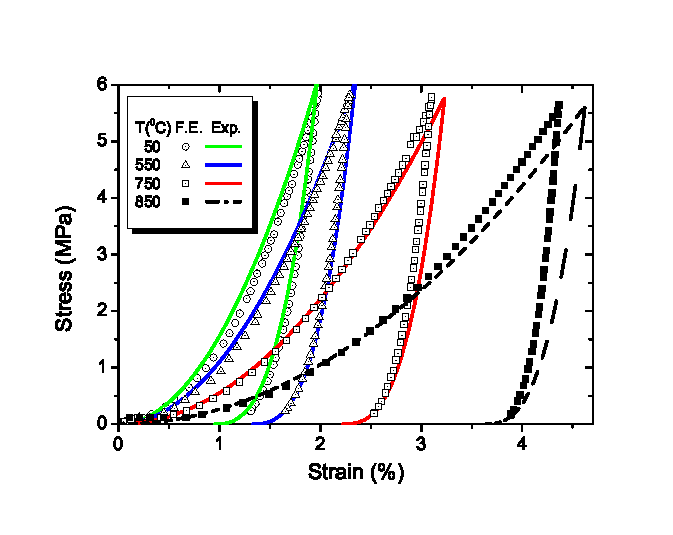
\includegraphics[width=0.5\textwidth]{chapters/figures/Fig-2}
\caption{Example of uniaxial compression testing results compared with predictions from material constitutive equations for lithium orthosilicate pebble beds at different temperatures \cite{Gan:2008kx}.}
\label{fig:UCT}
\end{center}
\end{figure}

Phenomenological models, derived from the volumes of collected data, have been proposed to describe the aforementioned mechanical behavior of the pebble beds with a conventional continuum-based approach. The continuum approach allows treatment of the pebble beds with standard finite element modeling (FEM). To employ FEM, mathematical models written in terms of average quantities and containing effective parameters are used. These models deduce a set of constitutive equations to be implemented in the framework of a finite element code.  There are two major variants of phenomenological modeling approaches developed among institutions, including: (1) A non-linear elastic model and a modified Drucker-Prager-Cap theory for plastic strain \cite{Gan2007189,fokkens2003}; and (2) A hyperporous non-linear elastic model and a Gurson model for plastic model \cite{DellOrco:2007hc,DellOrco:2010zr,DiMaio20081287}. The readers are referred to the additional efforts used in a third method\cite{fokkens2003} which employed two different elasticity laws for the loading and unloading branches but will not be discussed here. Alongside the development of the modeling techniques, several large scale pebble bed thermomechanics experiments were conducted in parallel. These experiments were intended to reveal the underlined thermo-mechanical characteristics of ceramic breeder pebble beds, and provide data for benchmarking the developed models.   The validation statuses as well as the features of the models are briefly described in the following section. 

Another modeling strategy is to model the pebble bed as a system of distinct interacting bodies that are subject to forces and resulting motions. This modeling approach called discrete element modeling (DEM) considers the mechanical interaction between pebbles and numerically solves the associated equations of motion \cite{An20072233,An20071393,Gan:2010uq,Gan20101782}. The DEM approach has recently received increased attention and the progress will be summarized to follow.

The review of the current status of development on the ceramic breeder pebble bed thermomechanics is organized as follows. In Section 2, current continuum modeling approaches and constitutive models for mechanical and thermal interactions are presented. In Section 3, a review of recent advancements on DEM is presented. A brief discussion on recently-initiated benchmarking efforts, in-pile experimental results, and other experimental observations relevant to pebble bed thermomechanics are given in Section 4. A proposed framework and a few conclusions on the outlook are drawn in Section 5. 


%%%%%%%%%%%%%%%%%%%%%%%%%%%%%%%%%%%%%%%%%%%%%%%%%%%%%%%%%%%%%%%%%%%%%%%%%%%%%%%%%%%%%%%%%%%%%%%%%%%%%%%%%%%%%%%%%%%%%%%%%%%%%%%%%%%%%%%%%%%%%%%%%%%%%%%%%%%%%%%%%%%%%%%%%%%%%%%%%%%%%%%%%%%%%%%%%%%%%%%%%%%%%%%%%%%%%%%%%%%%%%%%%%%%%%%%%%%%%%%%%%%%%%%


\section{Status of Continuum Modeling Approaches}
\subsection{Mechanical constitutive equations}
Continuum models focus on predicting global behavior, including volumetric strain and stress and the impact on the effective thermal conductivity, etc. Two institutions in Europe have spearheaded modeling efforts. One being Karlsruhe Institute of Technology, formerly FZK and referred to as such throughout this paper, and the other being ENEA-Brasimone with the Department of Nuclear Engineering at the University of Palermo, referred to as DIN throughout this paper. These two institutions have published a great deal of detail in regards to the specific details of their modeling techniques and the reader is referred to these publications for the fine points of the models \cite{DellOrco:2007hc,DellOrco:2010zr,DiMaio20101234,Gan2007189}. The discussion here calls attention to differences between models and attempts to serve as a reference basis for future modeling efforts.

The models from FZK and DIN share a common treatment of the mechanical interaction between the pebble beds with structural walls. In models from the two institutes, interfacial contact and friction forces are taken into account by application of the Coulomb friction law. This frictional contact law can be simply implemented in finite element code without considerable computation effort.

\subsubsection{FZK mechanical model}
In the FZK approach, the corresponding phenomenological constitutive models were developed based on the soil mechanics models implemented in the finite element code ABAQUS. This includes a non-linear elasticity model, which was originally developed for powder die compaction; a plastic strain model via a modified Drucker-Prager-Cap model, which was originally developed for soil mechanics; time-dependence via a consolidation creep law; and global thermal-mechanical coupling from material parameters.

The Drucker-Prager-Cap model captures the plasticity of the pebble beds and predicts the yielding and hardening behavior. A feature of the classic Druger-Prager-Cap model, as implemented in ABAQUS, is the ability to describe the plastic behavior of pebble beds under hydrostatic compression; a feature which is not present in classical metal plasticity models. However, researchers at FZK recognized that for materials with large creep strain amplitudes (e.g. beryllium pebble beds), hardening laws defined by default in ABAQUS were insufficient. Therefore, unique hardening laws were developed and implemented in place of the standard equations referenced in ABAQUS. An advantage gained from the redefined hardening laws is their capture of the creep behavior witnessed in pebble beds at high temperatures. The disadvantage of the Drucker-Prager-Cap model is the computational resources necessary for convergence of solutions. This has so far limited the FZK model to spatially two-dimensional simulations.

The main distinguishing feature unique to the continuum model developed in FZK is in their treatment of the material parameters that feed into the models described above. In particular, the hardening law in the model is manipulated to accommodate direct fitting to the oedometric tests. Unlike other continuum models, which require a trial-and-error method of optimizing numeric elasto-plastic parameters, the FZK model can be directly and clearly linked to experimental data. In this way, the model may be most adept at predicting behavior of a pebble beds where stress and temperature fields are very different from the controlled experiments which produced the constitutive relationships \cite{Gan2007189,Gan:2009vn,Gan:2010lh,Gan:2010kc}.

\subsubsection{DIN mechanical model}
The mechanical model established in the DIN model similarly assumes a non-linear elasticity model and a plasticity model. The non-linear elastic model assumes that during the reversible straining of a pebble bed, its effective logarithmic bulk modulus depends on the equivalent pressure according to a hypothesized power law. From this assumption as the foundation, DIN proceeds through a semi-theoretical derivation to relate the bed deformation modulus to the equivalent pressure; and stress state to volumetric strain. Included in the derivation are a number of effective parameter values. Values of all material parameters are chosen on an iterative trial-and-error basis until the model agreed well with the non-linear, elastic curves seen in oedometric experiments.

Attempting to resolve large computing time required when using the Drucker-Prager-Cap model for plastic deformation, DIN instead used a Gurson model. The Gurson model was originally developed for the analysis of pressure-dependent plastic behavior of mildly voided materials. The Gurson model postulates that the pebble bed behavior can be modeled as a continuous matrix in which stochastically-distributed voids are contained. In the Gurson model, compaction-related plastic deformation of the bed can to be reproduced. For material parameters in the Gurson model, again an iterative procedure was used until the model reproduced the results of relevant experimental tests. Lastly, in the consideration of the effective hardening law in pebble beds, a fifth order polynomial function was hypothesized. It should be noted that in the model's current form, it is incapable of directly capturing the creep behavior of pebble beds. However, the model was designed such that a future creep law could readily be implemented \cite{DellOrco:2007hc,DellOrco:2010zr,DiMaio20101234}.

The main advantage of the approach taken by DIN in their model is apparent when considering computational demand. DIN is currently able to model three-dimensional experiments with modest computer time. The most apparent drawback is the ad-hoc procedure of determining effective parameters used in the model. Without a direct link to experimental data, the applicability of the chosen effective parameters at predicting behavior beyond the range of the experimental conditions is unknown.

\subsection{Mechanics and heat transfer coupling}
Maintaining the breeder temperature within its temperature window is crucial for predictable performance and lifetime of the breeder unit. Proper temperature analysis requires careful characterization of thermal properties of the pebble beds. 

The pebble-bed experiments demonstrated that the effective thermal conductivity depends on the volumetric compressive strain; changes in thermal conductivity occurred between compacted and un-compacted systems. These measured phenomena indicate that thermo-mechanical modeling must also consider full, non-linear coupling between thermal and mechanical analysis.

The thermal models of the two institutions are fundamentally similar. The form of thermal model used by FZK follows from the experimental work carried out by J. Reimann from FZK in which empirical equations have been reported where the temperature and volumetric inelastic strain-dependence is incorporated into the bulk thermal conductivity. The thermal conductivity for a lithiated ceramic pebble bed over a specified range of temperature is reported in Ref.~\cite{Gan2007189} as:
\begin{align}\label{eq:fzkK}
k \left(W/m \cdot K \right)& = 1.81+0.0012  \,T - 5 \times 10^{ - 7} \,T^2 + \nonumber\\
&+ \big(9.03-1.386\times10^{-3} \,T-7.6\times10^{-6}\, T^2 + \nonumber\\
&+ 2.1\times10^{-9} \,T^3\big)\epsilon
\end{align}
where $T$ and $\epsilon$ are the local temperature and strain, respectively. The formula for thermal conductivity owes its functional form to the widely used Schlunder, Zehner, and Bauer (SZB) model. The coefficients in Eq.~\eqref{eq:fzkK} are empirically derived from experiments. The FZK model has  linked its constitutive equations directly to experimental data. 

In the DIN thermal model, the effective thermal conductivity has a quasi-linear dependence on volumetric strain and temperature. DIN reports the equation for determining thermal conductivity in Ref.~\cite{DellOrco:2007hc}, it is:
\begin{align}\label{eq:dinK}
k\left(W/m \cdot K \right)&=\lambda_0\left(1+\gamma T+\delta \epsilon\right)
\end{align}
where T and $\epsilon$ are the local temperature and strain, respectively. The relationship of Eq.~\eqref{eq:dinK} introduces several effective parameters, $\lambda_0$, $\gamma$, and $\delta$, that are determined from iterative fits to experimental data. Values of these effective parameters have been determined thus far for beryllium and certain lithium orthosilicate pebble beds\cite{DiMaio20101234}. The thermal conductivity, being a function of both thermal and mechanical parameters endows the models with a full coupling between thermo-mechanical analyses. 

\subsubsection{Thermal interface model}
The thermal interaction at the interface between pebble bed and containment wall is represented in both models as an effective heat transfer conductance, with only slight variations between the two approaches. In the FZK model, the thermal interaction is simulated with an effective heat transfer coefficient. The heat transfer coefficient (HTC) incorporates the combined effects of radiation heat transfer, pebble-solid conduction, and solid-gas heat transfer. Furthermore, in the event of a gap formation at the interface between pebble bed and containing surface, a separate heat transfer coefficient is employed. The researchers at DIN noted that interface conductance is affected by parallel paths of heat flow: pebble-wall conduction at contact areas and gas-wall convection. DIN therefore posits that the macroscopic phenomena can be modeled as a pressure-dependent thermal gap at the interface. They therefore have a thermal interface conductance that is a function of temperature, pressure, and local volumetric strain. An iterative trial-and-error method was also used to determine the effective parameters in this term. 


%%%%%%%%%%%%%%%%%%%%%%%%%%%%%%%%%%%%%%%%%%%%%%%%%%%%%%%%%%%%%%%%%%%%%%%%%%%%%%%%%%%%%%%%%%%%%%%%%%%%%%%%%%%%%%%%%%%%%%%%%%%%%%%%%%%%%%%%%%%%%%%%%%%%%%%%%%%%%%%%%%%%%%%%%%%%%%%%%%%%%%%%%%%%%%%%%%%%%%%%%%%%%%%%%%%%%%%%%%%%%%%%%%%%%%%%%%%%%%%%%%%%%%%



\section{Discrete Element Method}
Discrete Element Method (DEM) introduced by~\cite{Cundall1979} has been shown to be a promising tool to study the behavior of granular systems through the interaction between the individual particles. DEM has been used successfully to study the micromechanical aspects of pebble bed thermo-mechanics in the past~\cite{An20072233,Gan:2010uq}. Furthermore, DEM can be used to establish a relation between the microscopic interactions and the macroscopic response of the granular assemblies. Reference \cite{An20072233} studied the pebble assemblies in rectangular and cylindrical containers bounded by a elastic walls. The effect of packing factor, geometry of the assembly on the overall stress-strain response under uni-axial compression tests (UCT) has been thoroughly investigated. \cite{Gan:2010uq} have studied similar pebble assemblies in a cubic box with periodic boundary conditions. In both the above studies, a non-linear stress-strain response and a characteristic residual strain after unloading (analogous to plastic strain in continuum systems) has been observed akin to the experimental results~\cite{Reimann:2000tw}. It has been shown that the average coordination number, average normal contact force and the maximum normal contact force in the assembly has a unique functional relation (nonlinear, linear and linear, respectively) with the hydrostatic pressure or the applied pressure independent of the packing factor~\cite{Gan:2010uq,An20071393}. These functional relations may be used as master curves for the micro-macro correspondence in the pebble bed thermo-mechanics studies. A first attempt to include the creep mechanism in DEM has been made by~\cite{An20071393} showing the experimentally observed phenomenon such as the reduction of creep strain rate over time under constant load, albeit qualitatively. Further advances in the thermo-mechanics of pebble beds using DEM are under progress at KIT and UCLA in collaboration with experiments.

Recently, the effect of the pebble size distribution on the overall thermo-mechanical behavior of the pebble assembly is studied by~\cite{Annabattula2011} considering the pebble size distribution of ceramic breeder pebbles (Orthosilicate (OSi) pebbles) with a diameter range of $0.25~\mathrm{mm}$-$0.65~\mathrm{mm}$. Figure~\ref{fig:pebble-assembly-potential-energy} shows a binary pebble assembly in a periodic box. The colors indicate stored elastic strain energy of the pebble (red: maximum and blue: zero). The assembly has a maximum pebble radius $\rmax=0.25$ mm with the pebble size ratio $\rstar=\rmin/\rmax=0.6$, relative volume fraction $\vstar=\vmax/V=0.7$ and a packing factor $\eta=0.643$. The average stress in a granular assembly can be deduced from the contact forces between individual grains.

Another aspect of interest in the study of mechanics of pebble beds is the crush behavior of individual pebbles and their impact on the over all pebble bed response. DEM is used to study the behavior of a crushable pebble assembly with the crush load data for OSi pebbles (for individual pebbles) measured at KIT for pebbles of diameter 0.5 mm. 

A probabilistic method for analyzing the crush events of individual pebbles and a procedure with the combination of DEM and experimental data to obtain crush load probability has been reported by~\cite{Gan:2010kc}. Figure~\ref{fig:cdf_pebbles} shows the cumulative distribution function as a function of the hydrostatic pressure placed on the bed. The probability analysis, derived from DEM calculations, provides quantitative report of pebble crushing as a function of a specific hydrostatic pressure. The results of this analysis exemplify the growing strength of DEM techniques for analyses connecting global pebble bed loads to individual pebbles.

However, it has been shown~\cite{Zhao2010,Zhao2011} that a criterion based on critical stored elastic energy is the most suitable criterion for describing the OSi pebble failure. Hence, the crush load data (provided by fusion materials laboratory at KIT) has been transformed into equivalent elastic strain energy showing a Weibull distribution~\cite{Zhao2010}. This critical energy (randomly generated distribution) is used as the criterion for failure of pebbles in the DEM simulations. First, the assembly is loaded up to 3\% strain in uniaxial compression and then unloaded to a stress-free state. The elastic modulus of the pebble is reduced (from initial value to a small value of 1 kPa) with increase in elastic strain energy of the pebble according to a phenomenological damage accumulation law~\cite{Annabattula2011b}. The damage state is frozen at the end of loading step and hence there will be no further damage accumulation in the unloading step. 

Figure.~\ref{fig:stress-strain-effect} shows the results for two types of damage law each with three different realizations. Each realization corresponds to a different random distribution of critical energies assigned to the pebbles in the assembly. The results do not show appreciable sensitivity to random distribution of energies. In the case of gradual damage law, the reduction of the elastic modulus of the pebble starts when the stored elastic energy reaches 50\% of the critical energy for that pebble and the elastic modulus reaches exponentially to its minimum value when the stored elastic energy reaches the critical energy prescribed. In the case of sudden damage this reduction starts at a much later stage when the stored elastic energy reaches 95\% of the critical energy of the pebble. Clearly, the assembly with a sudden damage accumulation shows a higher maximum strength compared to the gradual damage. In the case of the gradual damage, the pebbles start to degrade much earlier (at small strain) than in the case of sudden damage. Hence the critical number of pebbles to fail for the onset of maximum strength is reached earlier (at small strain) in gradual damage. It turns out that a mere 0.2\% pebbles is the critical number for the onset of maximum strength (stress plateau) observed. 

The nature of damage evolution influences the maximum strength and strain at which the maximum strength is attained while the critical number of failed pebbles for this saturation is independent of the damage evolution law (also see~\cite{Zhao2010}). Also note that the high frequency oscillations during loading in the stress-plateau region represent the failure of new pebbles. The current analysis also shows a creep-like behavior of the stress-strain response and hence the stress-plateaus observed in the experiments~\cite{Reimann:2000tw} may indicate the presence of pebble crushing in addition to the thermal creep mechanism. Furthermore, the residual strain after unloading is large for the system with sudden damage than the system with gradual damage. It should be noted that the assembly with gradual damage has more number of damaged pebbles at the end of loading (at 3\% strain) making the assembly more compliant than in the case of sudden damage. 


%%%%%%%%%%%%%%%%%%%
\begin{figure}
\begin{center}
\begin{minipage}{0.45\textwidth}
\includegraphics[width=6cm]{chapters/figures/Fig-3}
\begin{picture}(15,15)(340,-120)
\put(330,-80){\includegraphics[scale=1]{chapters/figures/Fig-3b}}
\end{picture}
\end{minipage}
\end{center}
\caption{(color online) A binary pebble assembly with $\rstar = 0.6$ and $\vstar=0.7$ showing the stored elastic energy of the pebbles at $\epsilon_{33}=1.5\%$; pebbles of radius $r_s$ (small) and $r_g$ (large).}
\label{fig:pebble-assembly-potential-energy}
\end{figure}



\begin{figure}[!t]
  \begin{center}
\includegraphics[width=0.5\textwidth]{chapters/figures/Fig-4}
\end{center}
 \caption{(color online) Cumulative distribution functions for crushing of individual pebbles inside the bed for as-fabricated pebbles, calculated by (1) maximum contact forces and (2) all inter-particle contact forces~\cite{Gan:2010kc}.}
 \label{fig:cdf_pebbles}
\end{figure}


\begin{figure}[t!]
\begin{center}
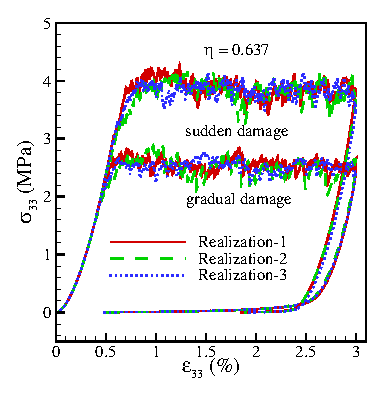
\includegraphics[width=0.4\textwidth]{chapters/figures/Fig-5}
\end{center}
\caption{(color online) Stress-Strain response of a granular assembly under uni-axial compression for two different damage evolution laws (gradual and sudden). Each damage evolution criterion is simulated with three different realizations of randomly prescribed critical failure energy for individual pebbles following Weibull distribution.}
\label{fig:stress-strain-effect}
\end{figure}



\section{Experimental Pebble Bed Thermomechanics Studies}
\subsection{Out-of-pile experiments}
The constitutive equations developed for finite element models were derived from the uniaxial compression experiments, which are not fully representative of fusion operating conditions. A more prototypical experiment should subject a pebble bed to isostatic loading. This could be generated by either an in-pile pebble bed experiment or by making use of differential thermal expansion between a pebble bed and its containing structure. The latter has been attempted with several out-of-pile experiments launched by the HE-FUS 3 facility at ENEA Brasimone. The experiments investigated the thermo-mechanical behavior of pebble beds within geometry much more representative of current breeder designs. These include the medium-scale mock-up exercises of HELICA (HE-FUS3 Lithium Cassette) and HEXCALIBER (HE-FUS3 Experimental Cassette of Lithium Beryllium Pebble Beds) \cite{dellorco:2006,DiMaio20081287}. For those experiments, the pebble layers are heated by electric heaters, and temperature and displacement were measured.

\subsubsection{FZK Benchmarking}
FZK has performed validation of their FEM code against the data collected from the HELICA experiment \cite{Gan:2008kx}. They have also reported the results of simulations of HEXCALIBER but have, as yet, not directly validated against the collected experimental data \cite{Gan:2009vn}.

In the HELICA experiment, the pebble beds experienced six thermal ramps, each applied for an hour, and then the pebble beds were actively cooled with a helium flow. After cooling, the pebble beds were subjected to the another thermal ramp and the process was repeated. DIN reports\cite{dellorco:2006} that the pebble bed temperatures exhibited cyclical behavior. FZK simulated two cycles of the HELICA test and an example of the calculated results and experimental data are shown in Fig.~\ref{fig:FZK_HELICAa} and Fig.~\ref{fig:FZK_HELICAb}. In Fig.~\ref{fig:FZK_HELICAa} we see temperature histories at a particular location (100 mm from the first wall) during a loading-unloading cycle. The simulation results follow the temperature increase during the thermal ramps up until the seventh hour, then again follow the experimental data as the test rig is cooled with the helium coolant. Even with the two-dimensional simplification of the model, there is excellent agreement between calculations and measurements. In Fig.~\ref{fig:FZK_HELICAb} the displacement calculated by FZK is also in strong agreement with the average of measured displacements for the entire duration of the heating-cooling cycle. Because of the overwhelming amount of computer time necessary for the FZK model to complete a fully three-dimensional and transient simulation, the FZK computations of HELICA and HEXCALIBER are carried out in two dimensions; the helium temperature is chosen at an average value of measured inlet and outlet temperatures.

From FZK's numeric simulation arise several important observations: (i) a three-dimensional analysis would provide more detail, spatial temperature variation of e.g. coolants would likely explain much of the deviation between temperature profiles predicted by the simulation and measured in the HELICA experiment; (ii) gap formations, with sizes on the order of a pebble diameter, were detected at the interface of the first wall in ceramic beds; (iii) the maximum hydrostatic pressures seen in the ceramic bed are anticipated to be above the fracturing limit of the lithium ceramic. The consequences of some of these observations, if true and real, are severe enough that they merit careful attention. Gap formation and pebble failure (crush or fracturing) are important topics that must be considered in validation with future experiments.

\subsubsection{DIN Benchmarking}
Because of the characteristics of the DIN model, full three-dimensional simulations were capable of being relatively easily performed. In the framework of benchmarking efforts, DIN has performed validation of their model against experimental results of HELICA, shown in Fig.~\ref{fig:DIN_HELICA} as well as HEXCALIBER, shown in Fig.~\ref{fig:DIN_HEX}.

The results of the DIN model show also strong agreement to the experimental results of HELICA as demonstrated in one example of temperature histories shown in Fig.~\ref{fig:DIN_HELICA}. In this profile, the same location as that modeled by FZK (100 mm from the first wall) is simulated by DIN. The FEM simulations from DIN (Fig.~\ref{fig:DIN_HELICA}) are reported over the six-hour heating portion of a single heating ramp cycle of HELICA. When comparing the results from DIN with those of FZK (in Fig.~\ref{fig:FZK_HELICAa} and Fig.~\ref{fig:FZK_HELICAb}) we see the DIN model has slightly better predictive capabilities for the temperature histories. This may be due attributed to the three-dimensional variations in coolant temperature being captured by the DIN model. 


\begin{figure}[t!]
\centering
\includegraphics[width=0.5\textwidth]{chapters/figures/Fig-6}
\caption{Results of the FZK benchmarking with HELICA\cite{Gan:2009vn} showing temperature variations with time during a loading cycle (T in $^\circ$C) at 100 mm from FW.}\label{fig:FZK_HELICAa}
\end{figure}

\begin{figure}[t!]
\centering
\includegraphics[width=0.5\textwidth]{chapters/figures/Fig-7}
\caption{Results of the FZK benchmarking with HELICA\cite{Gan:2009vn} showing a comparison of displacements (in mm) in HELICA between calculated and measured LVDT values.}
\label{fig:FZK_HELICAb}
\end{figure}

Unfortunately, the ambitions of HEXCALIBER were limited due to the crippling of several heaters. Nevertheless, the limited data was still used in efforts to validate the constitutive relationships of the DIN model. The temperature variations with time were the only major result reported by the ENEA Brasimone team, such as that shown in Fig.~\ref{fig:DIN_HEX}; mechanical results are still forthcoming from the research group. From the comparisons to experimental measurements in HELICA and HEXCALIBER it is encouraging to notice that even in the absence of a creep model, satisfactorily close agreement were seen between computation and measurement. So far, no detailed displacement comparisons have been made to experimental data.

Several important observations are also made from the results of the DIN simulation: (i) three-dimensional effects were important to calculations of the convective energy transport of the helium coolant; future models should continue to be analyzed in three-dimensions; (ii) DIN reports that in HELICA all ceramic beds experience a compressive force everywhere and no gap formation is ever detected. 

In summary, the benchmarking efforts have only recently begun in Europe. A typical pebble bed thermomechanics simulation involves first calculating overall temperature fields of the blanket unit as it undergoes volumetric nuclear heating as well as cooling at the boundaries. The non-linear mechanical analysis is then performed for stress and strain estimations. However, since the effective thermal conductivity of the ceramic breeder pebble bed is, to some degree, dependent on strain, a coupled thermal and mechanical analysis is needed. Additional details on modeling steps can be found in Refs.~\cite{DellOrco:2010zr,DiMaio20081287,DiMaio20101234,Gan:2009vn,Gan:2010lh,dellorco:2006}. The two most developed models, from FZK and DIN, have had their results compared to experimental data and have thus far shown great promise. 

However, it must be noted that the benchmarking efforts are incomplete and inconsistencies between the two models must be explained as they move forward. For example, the model of FZK concluded that a gap appeared between the pebble bed and structural wall, however the model from DIN reported no gap formation. The existence of a gap between pebble bed and structural wall will negatively affect the ability to cool the pebble bed and thereby impact structural and tritium release properties of the bed. That such a discrepancy exists between calculated results of the models on such a critical feature warrants either more benchmarking efforts or a careful deconstruction of the constitutive equations to discover the source of the inconsistency. Future experiments aimed at benchmarking ought to focus on creating apparatus capable of expressing, among other things, when gap formation or pebble failure occurs.


\begin{figure}[t!]
\begin{center}
\includegraphics[width=0.4\textwidth]{chapters/figures/Fig-8}
\caption{Exemplary results of the DIN benchmarking with HELICA: Temperature variations with time during a loading cycle at 100 mm from FW\cite{DellOrco:2007hc}.}
\label{fig:DIN_HELICA}
\end{center}
\end{figure}


 \begin{figure}[t!]
\begin{center}
\includegraphics[width=0.4\textwidth]{chapters/figures/Fig-9}
\caption{Exemplary results of the DIN benchmarking with HEXCALIBER : Temperature variations with time during a loading cycle within the first lithium-orthosilicate cell\cite{DellOrco:2010zr}.}
\label{fig:DIN_HEX}
\end{center}
\end{figure}



\subsection{Pebble bed assemblies experiment}
The pebble bed assemblies (PBA) experiment is designed to study the effect of neutron irradiation on the thermo-mechanical behavior of a ceramic breeder pebble-bed under DEMO representative thermo-mechanical loads \cite{Magielsen2007,magielsen2005,sander2011}. This was accomplished via analysis of changes of the in-pile temperature profiles during irradiation as wall as from the post irradiation examination of the pebble bed in the Hot Cells. Within the assemblies, there are four test elements; each resembling a small-scale mock-up of a HCPB TBM with a ceramic breeder pebble bed sandwiched between two beryllium pebble beds. Before irradiation, the beds are pre-compacted with a compressive load of 3 MPa to ensure good settling and contact.  

FEM analysis was performed to study pre-compaction procedures.  During progressive irradiation, temperatures are recorded at several locations in the ceramic breeder bed as well as other critical positions. Reviewing the recorded temperature data, when comparing the temperature in the center of the ceramic breeder pebble bed during later cycles and earlier cycles there appears to be a decrease in temperature for the exact same environmental conditions. Changes in the pebble beds and their characteristics are examined both in-pile by neutron radiography and out-of-pile by e.g. SEM during post-irradiation examination (PIE). The estimated bed height reduction from neutron radiographies over the course of the irradiation has shown 3\% of creep compaction. 

A pebble bed experiencing creep compaction is both becoming more dense as well seeing more-developed inter-pebble conduction paths. The effective thermal conductivity for a creep-compacted ceramic pebble bed is thus expected to be higher than a standard ceramic pebble bed. This phenomenon results in lower temperature gradients and a lower overall temperature magnitude, which is precisely what was observed in the experiment over the course of the cycling. 

During PIE, various microscopy preparation techniques are used to study the deformation state of the pebble beds (signs of creep compaction and sintering), formation of gas gaps between the pebble beds and structural materials, and the interaction layers between eurofer-ceramic and eurofer-beryllium. 

Figure~\ref{fig:pba} shows the cross-section of Li$_2$TiO$_3$ pebbles (left) and Li$_4$SiO$_4$ pebbles (right) post irradiation. Evident in the images is sintering of the lithium titanite and significant fracturing of the lithium orthosilicate pebbles. Importantly, however, it must be noted that the pebble beds performed reliably in spite of the changes displayed in these images \cite{magielsen2011}. 


\begin{figure}[t!]
\centering
\includegraphics[width=0.5\textwidth]{chapters/figures/Fig-10}
\caption{Notable features of irradiated Li$_2$TiO$_3$ and Li$_4$SiO$_4$ pebble beds from PBA\cite{magielsen2011}. (Left) Demonstration of significant sintering of Li$_2$TiO$_3$ pebbles with no fracturing; the visible cracks originated from production and handling. (Right) Demonstration of cracking of Li$_4$SiO$_4$ pebbles.}
\label{fig:pba}
\end{figure}


\subsection{Other thermomechanics characterization experiments}
Coming from the standpoint that strain in a pebble bed is induced by thermal expansion, an experiment was conducted to characterize the pebble bed thermal expansion coefficient \cite{Tanigawa:2007fc}.  The thermal expansion coefficient of a packed \lit pebble bed is measured under a compressive load of 0.1MPa.  The study concludes that for beds with packing factors of 65.3 to 68.5\%, the average thermal expansion coefficient was $(1.4\pm0.2)\times10^{-5}K^{-1}$. This thermal expansion coefficient of the pebble bed was equal to 78\% of that for the bulk material under the conditions used in the study. The reduction in thermal expansion coefficient is less significant than that of the effective modulus, which is more than 2 orders of magnitude smaller than the bulk value. 

The effect of thermal cycling on the packing state is of interest; in particular, it is foreseen that the ITER TBM will be subjected to such conditions. The question that arises is whether a void region will be created under thermal-cyclic loading due to the differential rates of expansion and contraction of the pebble bed and structural containing wall. This uncertainty was first addressed in an experimental set-up involving Li$_2$TiO$_3$ pebbles enclosed by two Kovar flanges while sandwiched between two commercial-grade CVD silicon carbide discs \cite{Calderoni:2006ye}. The set-up allows for generating a high stress through large differential in thermal expansion coefficients. The experimental results indicate that high thermal stresses and deformations are present during the initial thermal cycle of the assembled test article, but are successively alleviated due to a combination of pebble re-arrangement within the bed and creep induced deformation. This suggests that a few thermal cycles under a controlled atmosphere and a compressive load before final assembly of blanket sections would mitigate the severity of the thermal stresses during start-up. This is also shown in a later experiment, in which the increment of compression decreased with each heating cycle and became negligible after 30 cycles \cite{Tanigawa:2010cr}. Extrapolating the finding to a prototypical blanket breeder pebble bed design, the study concludes that for a height of 1 m long pebble bed, a 51 mm high cavity may be generated at the top of the bed with an initial packing of 65\% under thermal cyclic operations.  

\section{Pebble Bed Thermomechanics Summary \& Framework}
The progress already achieved holds the promise of a pebble bed thermomechanics framework that will contribute substantially to the success of the ceramic breeder blanket development. In this framework, the continuum modeling approach using FEM and empirically derived material constitutive equations is capable of correctly characterizing the stress load to which a breeder pebble bed unit may be subject during the operations as shown in Fig.~\ref{fig:framework}. The DEM approach analyzes this load and determines the possibility fraction of pebble cracking based on the crush load data of pebbles or the degree of sintering depending on the local contact stress. The combined analyses warrants a high confidence of success to the assembly and design of breeder units in a blanket.  Experiments should also be conducted to assess the manner of pebble relocations and packing rearrangement when pebble cracking occurs. Since there is no perfect packing state, it is important to learn if the breeder unit will continue to function in accord with the original design goals under all complex operating conditions.  The ultimate objectives of the pebble bed thermomechanics include to delineate a  near-equilibrium packing state as the initial state, quantify breeder unit thermomechanics parameters during operations, understand how these properties vary as packing state alters and the degree of variation, and ensure breeder functions as it is intended to in the fusion operational phase spaces.
\begin{figure}[t!]
\begin{center}
\includegraphics[width=0.5\textwidth]{chapters/figures/Fig-11}
\caption{Example Pebble Bed Thermo-mechanics Research Framework.}
\label{fig:framework}
\end{center}
\end{figure}

This leads to a more reliable blanket design. The analysis has preliminarily defined what peak stress values the breeder unit may be subjected to under the operations (e.g. $< 2-3$ MPa for Li$_4$SiO$_4$ or $< 5$ MPa for Li$_2$TiO$_3$). Since creep will lead to stress relaxation, further development incorporating creep models for high temperature DEM simulation is desired. This may increase the peak stress margin if stress relaxation is taken into account. Despite the scale of the experiments conducted so far, validation experiments are still necessary in regards to current continuum FEM models. Moreover, validation and refinement of simulations with regards to pebble damage crush properties are desired in particular in view of damage mechanisms.  There may be merits to perform crush load tests for irradiated pebbles at operating temperature ranges (room to 850/900 $^\circ$C). It holds forth promising on the continued pebble bed thermomechanics study in fine details a higher confidence to the ceramic breeder lifetime performance in a blanket.  The quest is to define and search a persistent ceramic breeder packing state throughout the blanket lifetime. 


% Methodology
\chapter{Development of Discrete Element Method for Pebble Bed Solid Breeders}\label{ch:modeling-development}

In this chapter I will cover the background of the discrete element method (DEM), the physics governing interactions of the distinct grains in the numerical framework, and 

%%%%%%%%%%%%%%%%%%%%%%%%%%%%%%%%%%%%%%%%%%%%%%%%%%%%%%%%%%%%%%%%%%%%%%%%%%%%%%%%%%%%%%%%%%%%%%%%%%%%%%%%%%%%
%%%%%%%%%%%%%%%%%%%%%%%%%%%%%%%%%%%%%%%%%%%%%%%%%%%%%%%%%%%%%%%%%%%%%%%%%%%%%%%%%%%%%%%%%%%%%%%%%%%%%%%%%%%%
%
% new section
%
%%%%%%%%%%%%%%%%%%%%%%%%%%%%%%%%%%%%%%%%%%%%%%%%%%%%%%%%%%%%%%%%%%%%%%%%%%%%%%%%%%%%%%%%%%%%%%%%%%%%%%%%%%%%
%%%%%%%%%%%%%%%%%%%%%%%%%%%%%%%%%%%%%%%%%%%%%%%%%%%%%%%%%%%%%%%%%%%%%%%%%%%%%%%%%%%%%%%%%%%%%%%%%%%%%%%%%%%%
\section{Grain-scale Modeling} \label{sec:modeling-dem}

The observable, macroscopic behavior of particulate, or granular, systems is a complex function of myriad particle interactions. Historically, empirical relationships have been used to describe these systems as if a continuous media, \textit{e.g.} the correlations for heat transfer discussed in \cref{sec:granular-ht-correlations}. But with the advent of the discrete element method by Cundall and Strack and the acceleration of computing power, it became practical to investigate these particulate systems at the particle scale without continuum assumptions \cite{Cundall1979}. With DEM, we track all the particles in the system in a Lagrangian manner. In the ensemble, the kinematics of each particle is tracked and updated based on balances (or imbalances) of forces or energy acting upon the particle. In this section I will work through equations governing interaction of particles in the DEM framework, the methods of computation, and the code used for implementation.



%~~~~~~~~~~~~~~~~~~~~~~~~~~~~~~~~~~~~~~~~~~~~~~~~~~~~~~~~~~~~~~~~~~~~~~~~~~~~~~~~~~~~~~~~~~~~~~~~~~~~~~~~~~~
% new subsection
%~~~~~~~~~~~~~~~~~~~~~~~~~~~~~~~~~~~~~~~~~~~~~~~~~~~~~~~~~~~~~~~~~~~~~~~~~~~~~~~~~~~~~~~~~~~~~~~~~~~~~~~~~~~
\subsection{Particle Dynamics}\label{sec:particle-dynamics}

The grains in our system are allowed translational and rotational degrees of freedom. In a packed bed, we can restrict our attention to local forces between particles; neglecting, say, non-contact forces such as van der Waals or electrostatic forces. In the first construct of momentum and temperature consideration, the particles are treated as if in vacuum. However a derivation of fluid interaction forces will be given in \cref{sec:modeling-cfd-dem}.

Assuming we know the contact forces acting upon particle $i$, Newton's equations of motion are sufficient to describe the particle kinematics. For translation and rotational degrees of freedom, the equations are:,
\begin{subequations}
\label{eq:newtons-second}
\begin{align}
	m_i  \ddt{\vec{r}_i}   & = m_i\vec{g} + \vec{f}_i \label{eq:newton-translational} \\
	I_i\dt{\vec{\omega}_i} & = \vec{T}_i \label{eq:newton-rotational}
\end{align}
\end{subequations}
where $m_i$ is the particle mass, $\vec{r}_i$ its location in space, $\vec{g}$ is gravity, $I_i$ is the particle's moment of inertia, and $\vec{\omega}_i$ its angular velocity.

The net contact force, $\vec{f}_i$, represents the sum of the normal and tangential forces from the total number of contacts, $Z$, acting on this grain.
\begin{equation}
 	\vec{f}_i = \sum_{j=1}^{Z} \vec{f}_{n,ij} + \vec{f}_{t,ij}
 \end{equation} 
and the net torque, $\vec{T}_i$, is similarly,
\begin{equation}
	\vec{T}_i = -\frac{1}{2}\sum_{j=1}^{Z} \vec{r}_{ij} \times \vec{f}_{t,ij}
\end{equation}

When Cundall and Strack first proposed the discrete element method, they used a linear spring-dashpot structure which saw the normal and tangential forces written as,
\begin{subequations}
\label{eq:dem-forces}
\begin{align}
	\vec{f}_{n,ij} &= k_{n,ij} \delta_{n,ij}\vec{n}_{ij} - \gamma_{n,ij} \vec{u}_{n,ij} 	\label{eq:normal-force} \\
	\vec{f}_{t,ij} &= k_{t,ij} \delta_{t,ij}\vec{t}_{ij} - \gamma_{t,ij} \vec{u}_{t,ij} 	\label{eq:tangential-force}
\end{align}
\end{subequations}
where Cundall and Strack defined the stiffness coefficients $k$ as constants and local damping coefficients $\gamma$ were proportional to them, $\gamma \propto k$, to allow dissipation of energy and the system to reach an equilibrium. 

Relative normal and tangential velocities, respectively, are decomposed from particle velocities,
\begin{subequations}
\label{eq:dem-velocities}
\begin{align}
	\vec{u}_{n,ij} &= (-(\vec{u}_i-\vec{u}_j)\cdot\vec{n}_{ij})\vec{n}_{ij} \\
	\vec{u}_{t,ij} &= (-(\vec{u}_i-\vec{u}_j)\cdot\vec{t}_{ij})\vec{t}_{ij}
\end{align}
\end{subequations}
with the unit vector $\vec{n}_{ij}$ pointing from particle $j$ to $i$

Similarly to the approach of Hertz (see \cref{sec:hertz-theory}), the surfaces of the two particles are allowed to virtually pass through each other (no deformation) resulting in normal and tangential overlaps of,
\begin{subequations}
\label{eq:dem-overlaps}
\begin{align}
	\delta_{n,ij} &= (R_i + R_j) - (\vec{r}_i -\vec{r}_j)\cdot \vec{n}_{ij} \\
	\delta_{t,ij} &= \int_{t_{c,0}}^{t} \vec{u}_{t,ij}\,\mathrm{d}\tau 
\end{align}
\end{subequations}
where the fictive tangential overlap, $\delta_{t,ij}$, is truncated to so the tangential and normal forces obey Coulomb's Law, $\vec{f}_{t,ij} \le \mu_i \vec{f}_{n,ij}$ with $\mu$ as the coefficient of friction of the particle.

The result is a relatively simple approach of calculating interaction forces between particles with \Cref{eq:dem-forces} based on the kinematics of velocity and position of interacting particles from \Cref{eq:dem-velocities} and \Cref{eq:dem-overlaps}, respectively. As DEM evolved and drew attention of more researchers, more complex formulas governing the spring-dashpot coefficients of \Cref{eq:dem-forces} emerged. But the core approach remained the same and the models all fall into the same family of so-called `soft particle' models of DEM. A well-composed summary of the different DEM force models is given by Zhu\etal.\cite{Zhu2007}

The method used in this work fits into the computational skeleton of Cundall and Strack's method but with non-linear spring-dashpot coefficients defined by simplified Hertz-Mindlin-Deresiewicz model. In this model, normal-direction stiffness coefficient of \Cref{eq:normal-force} is based on the Hertzian contact law (derived explicitly in \cref{sec:hertz-theory}). The tangential-direction stiffness coefficient follows from Brilliantov \cite{Brilliantov1996, Zhu2007, Langston1995}. Together, the spring coefficients are,
\begin{subequations}
\begin{align}
	k_{n,ij} &= \frac{4}{3}E_{ij}^*\sqrt{R_{ij}^*\delta_{n,ij}} \\
	k_{t,ij} &= 8 G_{ij}^*\sqrt{R_{ij}^*\delta_{t,ij}}
\end{align}
\end{subequations}
where $E_{ij}^*$ is the pair Young's modulus, $G_{ij}^*$ is the pair bulk modulus, and $R_{ij}^*$ is the relative radius. The terms are defined as,
\begin{subequations}
\begin{align}
	\frac{1}{E^*} &= \frac{1-\nu_1^2}{E_1} + \frac{1-\nu_2^2}{E_2} \\
	\frac{1}{R^*} &= \frac{1}{R_1} + \frac{1}{R_2} \\
	\frac{1}{G^*_{ij}} &= \frac{2(2+\nu_i)}{E_i} + \frac{2(2+\nu_j)}{E_j}
\end{align}
\end{subequations}

Similar to Cundall \& Strack's formulation, damping coefficients, $\gamma$, are included to account for energy dissipated from the collision of two particles \cite{DiRenzo2004, Tsuji1992, Tsuji1993}. Whether the damping coefficient is local or global and the exact form of the coefficient is more important for loosely confined granular systems and dictates the way the system approaches an equilibrium state.\cite{Makse2004} For the case of our tightly packed pebble beds, it suffices to use the efficient form of Refs.\cite{Dippel1996, Makse2004, Brilliantov1996, Zhang2005, Zhu2007},
\begin{subequations}
\begin{align}
	\gamma_n &= \sqrt{5}\beta_\text{diss}\sqrt{m^*k_{n,ij}} \\
	\gamma_t &= \sqrt{\frac{10}{3}}\beta_\text{damp}\sqrt{k_{t,ij} m^*}
\end{align}
\end{subequations}
with $\beta_\text{damp}$ as the damping ratio, and the pair mass, $\frac{1}{m^*} = \frac{1}{m_i} + \frac{1}{m_j}$. For a stable system with $\beta_\text{damp} < 1$, the damping ratio is related to the coefficient of restitution, $e$, as
\begin{equation}
	\beta_\text{diss} = -\frac{\ln{e}}{\sqrt{\ln^2{e}+\pi^2}}
\end{equation}

Systems to be solved by DEM models are therefore well-defined after specifying the few material properties of $E$, $\nu$, $\rho$, and $R_p$ and the interaction properties of $\mu$ and $e$.

Having expressed the contact mechanics of the discrete element method, we now must integrate the kinematic equations of the particles to resolve their evolutions. The most common means of marching in time with DEM is the velocity-Verlet algorithm \cite{Kruggel-Emden2008}. In this algorithm, \Cref{eq:newtons-second} are integrated with half-steps in velocity, full steps in position, and then finally the full step in velocity. In practice, the two half-steps in velocity are often compressed into a single, full step. The computational time integration steps are given in explicit detail in \cref{sec:dem-stability}. Owing to the explicit nature of the velocity-Verlet algorithm, stability is a constant concern with DEM simulations. Stable, critical time steps and means of circumventing unreasonably small time steps will also be addressed in \cref{sec:dem-stability}.

A last note. Throughout this work, I required a fully quiesced bed to act as a starting point or demarcate a mechanically steady-state bed. To determine when this occurs, the total kinetic energy of the entire ensemble is monitored and a packed bed is considered to have completely settled once the kinetic energy of the system is less than $10^{-8}$. A similar process was independently determined in a similar matter in the work of Ref.~\cite{Silbert2002}. 



%~~~~~~~~~~~~~~~~~~~~~~~~~~~~~~~~~~~~~~~~~~~~~~~~~~~~~~~~~~~~~~~~~~~~~~~~~~~~~~~~~~~~~~~~~~~~~~~~~~~~~~~~~~~
% new subsection
%~~~~~~~~~~~~~~~~~~~~~~~~~~~~~~~~~~~~~~~~~~~~~~~~~~~~~~~~~~~~~~~~~~~~~~~~~~~~~~~~~~~~~~~~~~~~~~~~~~~~~~~~~~~
\subsection{Granular Heat Transfer}\label{sec:dem-heat-transfer}

In a way analogous to handling particle momentums with Newton's laws of motion, Lagrangian tracking of energy of each particle is obtained via the first law of thermodynamics. Each particle is treated as a single distinct object and thus internal temperature gradients are assumed negligible. The temperature of particle $i$ is governed by
\begin{equation}\label{eq:thermoFirstLaw}
	m_iC_i\ddt{T_i} = Q_{s,i} + Q_{i}
\end{equation}
where $m$ and $C$ are the mass and the specific heat of the solid, respectively. Heat generation inside the particle is input with $Q_{s}$ and the total heat transferred to/from particle $i$ via conduction to all, $Z$, neighboring particles, is
\begin{equation}
	Q_i = \sum_{j=1}^Z Q_{ij}
\end{equation}

Assuming the particles are spherical, smooth, elastic, in vacuum, and we neglect radiation transfer between them, for two particles at temperatures $T_i$ and $T_j$, we quantify the amount of energy transferred between them with a contact conductance, $H_c$:
\begin{equation}\label{eq:pebble-conduction-heat-transfer}
    Q_{ij} = H_{c}(T_i - T_j)
\end{equation}

Batchelor and O'Brien\cite{Batchelor1977} developed a formulation of similar form and then made the brilliant observation that the temperature fields in the near-region of contacting spheres are analogous to the velocity potential of an incompressible, irrotational fluid passing from from one reservoir to another through a circular hole in a planar wall separating the two reservoirs. With the analogy, they could make use of the fluid flow solution to write the total heat flux across the circle of contact as \Cref{eq:pebble-conduction-heat-transfer} with heat conductance 
\begin{equation}\label{eq:batchelor-pebble-conductance}
    H_c = 2k_sa
\end{equation}
where $k_s$ is the conductivity of the contacting solids and $a$ is the radius of contact. Because we have assumed smooth, elastic, spherical solids, with Hertz theory (see \cref{sec:hertz-theory}), contact radius can be found as a function of contact normal force, $F_n$,
\begin{equation}
    a =  \left(\frac{3}{4}\frac{R^*}{E^*}\right)^{1/3}F_n^{1/3} 
\end{equation}
where, as before, $\frac{1}{E^*} = \frac{1-\nu_1^2}{E_1} + \frac{1-\nu_2^2}{E_2}$ and $\frac{1}{R^*} = \frac{1}{R_1} + \frac{1}{R_2}$. 

In the development of \Cref{eq:batchelor-pebble-conductance}, Batchelor and O'Brien had assumed the two contacting spheres to be of equal conductivity, $k_s$. Cheng\etal\cite{Cheng19994199} proposed a slightly modified conductance which allows for contacting materials of different thermal conductivity. They give,
\begin{equation}\label{eq:cheng-modification-batchelor}
    H_c = 2k^*a = 2k^* \left(\frac{3}{4}\frac{R^*}{E^*}\right)^{1/3}F_n^{1/3}
\end{equation}
where $\frac{1}{k^*} = \frac{1}{k_i} + \frac{1}{k_j}$. As well as being a more general, flexible formulation, the models analyzed by Cheng\etal\cite{Cheng19994199} are in good agreement with experiments.

Batchelor and O'Brien developed \Cref{eq:batchelor-pebble-conductance} with the assumption of two contacting particles in vacuum but, once developed, showed\cite{Batchelor1977} that this form is still valid when immersed in a fluid providing that the thermal conductivity ratio, $\kappa = \frac{k_s}{k_f}$, of solid and fluid is well above unity. The condition is expressed as,
\begin{equation}\label{eq:conductance-validity-fluid}
    \frac{a}{R^*} \kappa \gg 1
\end{equation}
The term $\frac{a}{R^*}$, from \cref{sec:hertz-theory}, is necessarily less than 1 for Hertz theory to be applicable. Thus for fluid in vacuum, the condition is identically satisfied but we must consider inaccuracies if we introduce an interstitial fluid with low conductivity ratios; for lithium ceramics in helium, the ratio is approximately $\kappa \approx 10$.

We step back from contact of a single pair of particles and consider a particle in an ensemble with many contacts. We must again consider the validity of applying \Cref{eq:cheng-modification-batchelor} at each contact. Vargas and McCarthy\cite{Vargas2002a}, propose introducing a conduction Biot number to relate resistance of heat transfer internal to a particle with resistance between particles,
\begin{equation}
    \Bi_c = \frac{H_c}{k^* d_p} = 2\frac{a}{d_p}
\end{equation}

Then if $\Bi_c \ll 1$, the individual energy transferred between each point of contact can be decoupled. The Biot number criteria is already satisfied for Hertz theory to be valid; having assumed that $\frac{a}{d_p} \ll 1$. Therefore the total heat transferred out of a single particle with $Z$ contacts, due to contact conductance, is the summed contribution of individual contacts, 
\begin{equation}
    Q_i = \sum_j^Z Q_{ij}
\end{equation}

Conductive heat transfer to neighboring particles comes from inter-particle conductance formulas. The form of contact conductance we use, from \Cref{eq:cheng-modification-batchelor}, which is built upon the solution of Batchelor and O'Brien\cite{Batchelor1977}, has been implemented by others in a variety of DEM studies\cite{Vargas2001, Chaudhuri2006, Zhou2009,Cheng19994199}. However, it should noted that in many other fields, the researchers are interested in such things as the parallel conduction through a stagnant interstitial gas\cite{Bu2013} or the temporary conduction during impact of fluidized beds\cite{Zhu2008,Zhang2011,Wu2011,Li2000}. In such cases, the formula for conductance can be quite different but are not appropriate for the physics of our packed beds. 


\subsubsection{Thermal Expansion}
The stresses predicted to act upon the solid breeder volume during operation of the fusion reactor arise from the differential rate of thermal expansion from the highly heated ceramic volume and the relatively cool structural container. Moreover, thermal settling motion is observed in pebble beds with cyclic heating \cite{Tanigawa:2010cr, Vargas2007, Chen2009, Divoux2008}. Both of those phenomena originate from effects of thermal expansion of individual particles in the ensemble. Therefore, I introduce a simple thermal expansion method into the DEM structure that updates the diameter of each particle as,
\begin{equation}
	d_{p,i} = d_{p_0,i}\left[1+\beta_i\left(T_i - T_0\right)\right]
\end{equation}
where $\beta_i$ is the thermal expansion coefficient (in units of \SI{1}{\per\kelvin}), $T_i$ is the temperature of the pebble at the current step, and $d_{0,i}$ is the initial diameter of the pebble at temperature $T_0$. The update of pebble diameter based on thermal expansion could be computed at every time step as it is not computationally expensive. All the same, I have left flexibility in the code to allow the computation at an arbitrary interval of time, typically every $\frac{N}{\Delta t} = \frac{10^4}{10^{-7}}$ in most models of ceramic pebble beds).



%~~~~~~~~~~~~~~~~~~~~~~~~~~~~~~~~~~~~~~~~~~~~~~~~~~~~~~~~~~~~~~~~~~~~~~~~~~~~~~~~~~~~~~~~~~~~~~~~~~~~~~~~~~~
% new subsection
%~~~~~~~~~~~~~~~~~~~~~~~~~~~~~~~~~~~~~~~~~~~~~~~~~~~~~~~~~~~~~~~~~~~~~~~~~~~~~~~~~~~~~~~~~~~~~~~~~~~~~~~~~~~
\subsection{Numerical Implementation of DEM}\label{sec:dem-solver}

The primary computational tool used in this study is LAMMPS (Large-scale Atomic/Molecular Massively Parallel Simulator) \cite{Plimpton1995}, a classical molecular dynamics code. The package of code, maintained by Sandia National Labs (http://lammps.sandia.gov), has many features making it particularly attractive for our use of granular material simulations. LAMMPS is open-source and written in highly-portable C++ allowing customization of any core modeling feature. LAMMPS runs with distributed-memory message-passing parallelism (MPI) and provides simple control (manual or automatic) of the spatial-decomposition of simulation domains for parallelizing. Perhaps most importantly, LAMMPS provides an efficient method for detecting and calculating pair-wise interaction forces; the largest consumer of run-time in the DEM algorithm \cite{Plimpton1995}. We build the LAMMPS core as a library to allow coupling LAMMPS features to other numerical tools. I use the scripting language of Python (Python 2.7) to write parent routines that pass information between LAMMPS objects while accessing all of Python's numeric and scientific libraries (\textit{e.g.} NumPy and SciPy). 

LAMMPS by default provides a rudimentary method of modeling of granular particles (the term `granular' in LAMMPS vernacular simply differentiates the discrete element of molecules or atoms from larger-scale granular particles of powders or pebbles); LAMMPS has been used for studying granular material since at least 2001 when Silbert\etal~studied granular flow on inclined planes \cite{Silbert2001}. However, the usefulness of LAMMPS for studying granular systems was greatly enhanced by LIGGGHTS (LAMMPS Improved for General Granular and Granular Heat Transfer Simulations), a suite of modules included on top of LAMMPS. LIGGGHTS has many academic and industrial contributors from around the world, with the code maintained as open-source by DCS Computing, GmbH.

Briefly, some notable features that LIGGGHTS brings to the LAMMPS environment include: built-in Hertz/Hooke pair styles with shear history, mesh importing for handling wall geometry, moving meshes, stress analysis of imported meshes, a macroscopic cohesion model, a heat transfer model, and improved dynamic load balancing of particles on processors\cite{Kloss2011,Kloss2012}. Both LIGGGHTS and LAMMPS are distributed under the open-source codes under terms of the Gnu General Public License.\cite{FreeSoftwareFoundationInc.2007}




%%%%%%%%%%%%%%%%%%%%%%%%%%%%%%%%%%%%%%%%%%%%%%%%%%%%%%%%%%%%%%%%%%%%%%%%%%%%%%%%%%%%%%%%%%%%%%%%%%%%%%%%%%%%
%%%%%%%%%%%%%%%%%%%%%%%%%%%%%%%%%%%%%%%%%%%%%%%%%%%%%%%%%%%%%%%%%%%%%%%%%%%%%%%%%%%%%%%%%%%%%%%%%%%%%%%%%%%%
%
% new section
%
%%%%%%%%%%%%%%%%%%%%%%%%%%%%%%%%%%%%%%%%%%%%%%%%%%%%%%%%%%%%%%%%%%%%%%%%%%%%%%%%%%%%%%%%%%%%%%%%%%%%%%%%%%%%
%%%%%%%%%%%%%%%%%%%%%%%%%%%%%%%%%%%%%%%%%%%%%%%%%%%%%%%%%%%%%%%%%%%%%%%%%%%%%%%%%%%%%%%%%%%%%%%%%%%%%%%%%%%%
\section{Young's Modulus Implementation in DEM for Ceramic Pebbles}\label{sec:exp-reduction-factor}

In all past DEM efforts for ceramic breeders, the validity of Hertz theory (see \cref{sec:hertz-theory} and \cref{sec:modeling-dem}) for describing the inter-particle contact force as a function of fictitious overlap is assumed. In our experimental test stand for crushing individual pebbles, our equipment was able to record accurate measurements of the force-travel relationship for each pebble, providing us with an opportunity to study the validity of the Hertzian contact laws. 

The derivation of the Hertz force can be found on page~\pageref{eq:hertz-normal-force} but the result is given again here for reference:
\begin{equation*}
  F_{n,ij} = \frac{4}{3}E_{ij}^* \sqrt{R_{ij}^*} \, \delta_{n,ij}^{3/2}
\end{equation*}
and, again, the pair Young's modulus and radius are
\begin{align*}
\frac{1}{E^*} & = \frac{1-\nu_i^2}{E_i} + \frac{1-\nu_j^2}{E_j} \\
\frac{1}{R^*} & = \frac{1}{R_i} + \frac{1}{R_j}
\end{align*}

In experiments where we press a ceramic pebble between two anvils, we measure the travel, $s$, rather than the pebble overlap, so we modify \Cref{eq:hertz-normal-force} to be represented in terms of travel ($s = 2\delta$). Furthermore, for a pebble ($R_i = R_p$) in contact with a smooth plane ($R_j \rightarrow \infty$), the relative radius is simply $R^* = R_p = d_p/2$. We write the Young's modulus of the pebble as $E_p$ and for the test stand's anvil as $E_s$; similarly for the Poisson ratios of the two materials. The Hertz force acting upon a pebble between anvils is then expressed as a function of the pebble and anvil properties as,
\begin{equation}\label{eq:contact-force}
        F = \left[\frac{1}{3}\frac{\sqrt{d_p}}{\frac{1-\nu_p^2}{E_p} + \frac{1-\nu_s^2}{E_s}}\right] s^{3/2}
\end{equation}


\begin{figure}[!t]
\centering
\includegraphics[width = \singleimagewidth]{figures/hertz-dp-dependence}
\caption{Hertzian responses of \lit~pebbles compressed between platens. The colormap shows pebble diameters in \si{m}. The diameters span an order of magnitude from $d_p = \si{0.2 mm}$ to $d_p = \si{2 mm}$.}\label{fig:hertz-dp-dependence}
\end{figure}


The Young's modulus and Poisson ratio of the test stand are known values that do not vary between pebble experiments. Similarly, in the application of Hertz theory, we also assume the Young's modulus and Poisson ratio of the ceramic are also known, constant values. In that case, for any given pebble diameter, the term inside $[\quad]$ ought to be composed entirely of constants for any given pebble; there would therefore be a single force-travel response possible -- based only on $s$. Using the material properties given in Ref.~\cite{Gierszewski1998} for \lit, we plot a set of parametric curves based on diameter over a range of travel. The properties we have used for the nickel-alloy anvil of our test stand and \lit~are given in Table~\ref{tab:hertz-dp-study-props}. The curves are given in Fig.~\ref{fig:hertz-dp-dependence}.

\begin {table}[htp] %
\caption{Material properties used for \lit~and nickel-alloy platen}
\label {tab:hertz-dp-study-props} \centering %
\begin {tabular}{ cccccc }
\toprule %
$E_\text{peb}$      &     $\nu_\text{peb}$  &   $E_\text{stand}$        &     $\nu_\text{stand}$    \\
(GPa)           &                   &   (GPa)               &                   \\\toprule
126             &   0.24                &   220                 &   0.27                \\\bottomrule
\end{tabular}
\end{table}

Figure~\ref{fig:hertz-dp-dependence} shows that, for a given pebble diameter, that is strictly obeying Hertz theory, there is only a single force-displacement curve it can follow. However, when experiments are performed on single pebbles of \lis~we see responses such as shown in the dashed lines of Fig.~\ref{fig:fzk-exp-colormap}. Similarly for the dashed lines of \lit~in Fig.~\ref{fig:nfri-exp-curves}. The diameters of the pebbles are mapped to the given colormap.

Contrary to the diameter dependence seen in Fig.~\ref{fig:hertz-dp-dependence}, the curves of Figs.~\ref{fig:fzk-exp-colormap}, and~\ref{fig:nfri-exp-curves} do not demonstrate a pure relationship between diameter and force. For comparison, the solid lines on the figures for each ceramic show the predicted Hertzian response as calculated by \Cref{eq:contact-force} based on the measured diameter of each pebble. For both the \lis~and \lit~pebbles, there are very few pebbles that show a measured force-travel response that is similar to the Hertzian prediction based on the material properties reported in literature. I conclude that variations in pebble diameter can not alone account for the variations in the force curves measured for the pebbles in our experiments. I hypothesize instead that variation in measured curves is due to each pebble having a Young's modulus that is reduced from the values measured from sintered blocks as reported in literature. Therefore each pebble displays a different apparent Young's modulus in the single pebble experiments. 

The apparent Young's modulus of each pebble is rooted in the manufacture which yields pebbles with slightly different internal structures. The differences in internal structure then cause the pebble to behave with different stiffnesses than the value expected from measurements of sintered pellets of lithium ceramics. In fact, the solid lines in Figs.~\ref{fig:fzk-exp-colormap}, and~\ref{fig:nfri-exp-curves}, as calculated from the measurements of sintered pellets, appear to be an upper limit to the pebbles. Therefore I consider pebbles will emerge with values less than the value from literature, $E_\text{lit}$ by some factor between 0 and 1. To quantify the deviation of each pebble's $E_\text{peb}$ from the sintered pellet, I introduce a $\kappa$ factor, which I define as the softening coefficient:

\begin{equation}
\kappa = \frac{E_\text{peb}}{E_\text{lit}}
\end{equation}
where
\[
\kappa \in [0,1]
\]

If each pebble has a unique $\kappa$ value, it would quantify the spread in elastic responses seen in the experiments. The values are found by assuming that the pebbles are, in fact, behaving in a Hertzian manner and I can fit a Hertzian curve to our experimental measurements. This permits backing-out a $\kappa$ value, or in other words the unique $E_\text{peb}$ of that pebble. The sintered pebble value of Young's modulus for \lis~is taken to be $E_\text{lit} = \si{90~GPa}$ and the value for \lit~to be $E_\text{lit}= \si{124~GPa}$. Then I iterate over all values of $\kappa\in[0,1]$ and compare the Hertzian response to that pebbles force-displacement curve. At each iteration, the L2-norm of the difference between Hertzian and experimental curves is used as the `error'. The L2 norm, $A$ for a given array, $a$ is 

\begin{equation}
||A||_F = \left[\sum_{i,j}\textrm{abs}(a_{i,j})^2\right]^{1/2}
\end{equation}

This is a convenient way to compare the error at every point along the force-displacement curves. When the error is minimized, the softening coefficient value corresponding to the minimum is recorded for that pebble. The Hertzian curves (in black) for the \lis~and \lit~pebbles are plotted in green against the experimental curves in Figs.~\ref{fig:fzk-exp-hertz}, and~\ref{fig:nfri-exp-hertz}, respectively. 

Many of the curves for \lis~in Fig.~\ref{fig:fzk-exp-hertz} seem to be fit well with a Hertzian curve using a modified Young's modulus. The value of Young's modulus found for each pebble is ordered and plotted in Fig.~\ref{fig:fzk-E-plot}; the Young's modulus of pebble numbers 0 to 4 are the very soft pebbles seen with very low forces over the range of travel seen in Fig.~\ref{fig:fzk-exp-hertz}. The majority of pebbles, however, behave with a Young's modulus between 30 and 70 \si{GPa}. On the upper end, a few pebbles acted very similar to their sintered pellet counterpart with approximate value of 90 \si{GPa}. 

The two batches of \lit~pebbles analyzed (Fig.~\ref{fig:nfri-exp-hertz}) are similarly fit well to pebbles with modified Hertzian curves. The apparent Young's modulii of the \lit~pebbles are given in Fig.~\ref{fig:nfri-E-plot}. These \lit~pebbles have a large distribution of stiffness, from between 20 to 120~GPa for the 1~mm pebbles and roughly 2 to 80~GPa for the 1.5~mm pebbles.


The $\kappa$ factor for this batch of \lis~pebbles is also given as a histogram in Fig.~\ref{fig:fzk-kappa-hist}. For the \lis~pebbles, the histogram resembles a normal distribution but for the large spike in pebbles with very small $\kappa$. The four softest pebbles mentioned previously display relatively flat responses to travel before reaching a point where there is a sharp increase in the $F-s$ slope. In the experiments, the flat sections of the curve occurred when the pebbles in the anvil were not perfectly spherical and rotated slightly under the application of a small load. Once the pebbles rotated into a flat spot that could take a normal load without any angular moment, the force increased quickly under further travel. In light of this, it is unreasonable to consider their $\kappa$ values as representing their true stiffness which was only measured near the end of the F-s compression trial. Neglecting the four outliers in the histogram of Fig.~\ref{fig:fzk-kappa-hist}, we are then left with a distribution much more closely resembling a normal probability distribution.

The histograms for the two batches of \lit~are given in Fig.~\ref{fig:nfri-kappa-hist}. The distributions for both batches of \lit~pebbles more closely resemble Snedecor's F distribution with many pebbles behaving with a very small $\kappa$, then a long tail of few pebbles with large $\kappa$.

In Figs.~\ref{fig:fzk-kappa-dp-scatter} and~\ref{fig:nfri-kappa-dp-scatter} we see scatter plots of the pebble diameters against $\kappa$ values for the different batches of lithium ceramic pebbles. A Pearson Correlation value was calculated for each of the batches to quantify a correlation between diameter and $\kappa$. For the \lis~pebbles, we find $R = 0.198$ which is a weak positive correlation. For the \lit~pebbles we have $R = -0.385$ for $\bar{d}_p = 1$~mm and $R = -0.201$ for $\bar{d}_p = 1.5$~mm. Both of these are weakly negatively correlated. 

The results of these single pebble experiments indicate that the Young's modulus traditionally used in DEM simulations for ceramic pebble beds in solid breeders is incorrect. Numerical recreations of the probability distribution curves will be used to apply $\kappa$ to pebbles in the ensemble. From the weak correlations between diameter and $\kappa$, we are free to ignore any diameter dependence when assigning $\kappa$ values in the DEM framework especially in light of the current implementation of monodisperse pebble beds. Therefore, numerically, when assigning Young's modulii to the particles in the ensemble, the $\kappa$ distribution will be applied in a random fashion.

\begin{figure}[!t]
\centering
    \includegraphics[width=\doubleimagewidth]{figures/fzk-data-w-ideal-hertz.png}
    \caption{Dashed lines are \lis~pebbles of approximately \si{0.5 mm} diameter. Solid lines are the Hertzian (Eq.\ref{eq:contact-force}) responses based on each pebble's measured diameter.}
    \label{fig:fzk-exp-colormap}
\end{figure}

\begin{figure}
        \centering
        \begin{subfigure}[b]{\doubleimagewidth}
                \includegraphics[width=\textwidth]{figures/nfri-1mm-data-w-ideal-hertz.png}
                \caption{$\bar{d}_p = 1$ mm}
                \label{fig:nfri-1-exp-colormap}
        \end{subfigure}
        ~
        \begin{subfigure}[b]{\doubleimagewidth}
                \includegraphics[width=\textwidth]{figures/nfri-1.5mm-data-w-ideal-hertz.png}
                \caption{$\bar{d}_p = 1.5$ mm}
                \label{fig:nfri-1.5-exp-colormap}
        \end{subfigure}
        \caption{Dashed lines are \lit~pebbles. Solid lines are the Hertzian (Eq.\ref{eq:contact-force}) responses based on each pebble's measured diameter.}\label{fig:nfri-exp-curves}
\end{figure}


\begin{figure}[!t]
\centering
    \includegraphics[width=\doubleimagewidth]{figures/fzk-hertz-colormap.png}
    \caption{Force-displacement curves for \lis~pebbles (in color) along with their Hertzian fits (in black) calculated with each pebble having a unique Young's modulus.}
    \label{fig:fzk-exp-hertz}
\end{figure}

\begin{figure}
        \centering
        \begin{subfigure}[b]{\doubleimagewidth}
                \includegraphics[width=\textwidth]{figures/nfri-1mm-hertz-colormap.png}
                \caption{$\bar{d}_p = 1$ mm}
                \label{fig:nfri-1-exp-hertz}
        \end{subfigure}
        ~
        \begin{subfigure}[b]{\doubleimagewidth}
                \includegraphics[width=\textwidth]{figures/nfri-1.5mm-hertz-colormap.png}
                \caption{$\bar{d}_p = 1.5$ mm}
                \label{fig:nfri-1.5-exp-hertz}
        \end{subfigure}
        \caption{Force-displacement curves for \lit~pebbles (in color) along with their Hertzian fits (in black) calculated with each pebble having a unique Young's modulus.}\label{fig:nfri-exp-hertz}
\end{figure}

\begin{figure}[!t]
\centering
    \includegraphics[width=\doubleimagewidth]{figures/fzk-E-plot.png}
    \caption{Distribution of modified Young's modulus for a batch of \lis~pebbles. Most pebbles responded to compression with a Young's modulus well below the sintered pellet value of \si{90 GPa}.}
    \label{fig:fzk-E-plot}
\end{figure}

\begin{figure}
        \centering
        \begin{subfigure}[b]{\doubleimagewidth}
                \includegraphics[width=\textwidth]{figures/nfri-1mm-E-plot.png}
                \caption{$\bar{d}_p = 1$ mm}
                \label{fig:nfri-1mm-E-plot}
        \end{subfigure}
        ~
        \begin{subfigure}[b]{\doubleimagewidth}
                \includegraphics[width=\textwidth]{figures/nfri-1.5mm-E-plot.png}
                \caption{$\bar{d}_p = 1.5$ mm}
                \label{fig:nfri-1.5mm-E-plot}
        \end{subfigure}
        \caption{Distribution of modified Young's modulus for a batch of \lit~pebbles. All pebbles responded to compression with a Young's modulus well below the sintered pellet value of \si{126 GPa}.}\label{fig:nfri-E-plot}
\end{figure}


\begin{figure}[!t]
\centering
    \includegraphics[width=\doubleimagewidth]{figures/fzk-kappa-histogram.png}
    \caption{Histogram of $\kappa$ for a batch of \lis~pebbles. Most pebbles responded to compression with a Young's modulus well below the sintered pellet value of \si{90 GPa}.}
    \label{fig:fzk-kappa-hist}
\end{figure}

\begin{figure}
        \centering
        \begin{subfigure}[b]{\doubleimagewidth}
                \includegraphics[width=\textwidth]{figures/nfri-1mm-kappa-histogram.png}
                \caption{$\bar{d}_p = 1$ mm}
                \label{fig:nfri-1mm-kappa-hist}
        \end{subfigure}
        ~
        \begin{subfigure}[b]{\doubleimagewidth}
                \includegraphics[width=\textwidth]{figures/nfri-1.5mm-kappa-histogram.png}
                \caption{$\bar{d}_p = 1.5$ mm}
                \label{fig:nfri-1.5mm-kappa-hist}
        \end{subfigure}
        \caption{Histogram of $\kappa$ for two batches of \lit~pebbles. All pebbles responded to compression with a Young's modulus well below the sintered pellet value of \si{126 GPa}.}\label{fig:nfri-kappa-hist}
\end{figure}


\begin{figure}[!ht]
\centering
    \includegraphics[width=\doubleimagewidth]{figures/fzk-kappa-dp-scatter.png}
    \caption{Scatter of $\kappa$ against pebble diameter for a batch of \lis~pebbles showing almost no relationship between apparent stiffness and diameter.}
    \label{fig:fzk-kappa-dp-scatter}
\end{figure}

\begin{figure}
        \centering
        \begin{subfigure}[b]{\doubleimagewidth}
                \includegraphics[width=\textwidth]{figures/nfri-1mm-kappa-dp-scatter.png}
                \caption{$\bar{d}_p = 1$ mm}
                \label{fig:nfri-1mm-kappa-dp-scatter}
        \end{subfigure}
        ~
        \begin{subfigure}[b]{\doubleimagewidth}
                \includegraphics[width=\textwidth]{figures/nfri-1.5mm-kappa-dp-scatter.png}
                \caption{$\bar{d}_p = 1.5$ mm}
                \label{fig:nfri-1.5mm-kappa-dp-scatter}
        \end{subfigure}
        \caption{Scatter of $\kappa$ against pebble diameter for two batches of \lit~pebbles showing almost no relationship between apparent stiffness and diameter.}\label{fig:nfri-kappa-dp-scatter}
\end{figure}

\FloatBarrier


%~~~~~~~~~~~~~~~~~~~~~~~~~~~~~~~~~~~~~~~~~~~~~~~~~~~~~~~~~~~~~~~~~~~~~~~~~~~~~~~~~~~~~~~~~~~~~~~~~~~~~~~~~~~
% new subsection
%~~~~~~~~~~~~~~~~~~~~~~~~~~~~~~~~~~~~~~~~~~~~~~~~~~~~~~~~~~~~~~~~~~~~~~~~~~~~~~~~~~~~~~~~~~~~~~~~~~~~~~~~~~~
\subsection{Comparison of Young's Modulii Used in DEM Simulations}\label{sec:dem-studies-youngs-modulus}

The discrete element method is used by many ceramic breeder researchers to model the interaction of individual pebbles in an ensemble.\cite{An20071393, Lu2000, Zhao2010, Gan:2010uq, Annabattula2012a, VanLew2014} In the past studies, the Young's modulus of the ceramic materials used in DEM simulations was taken from historical data, for instance lithium metatitanate from Ref.~\cite{Gierszewski1998}. However, in the previous section I proposed a modification of the Young's modulus to be used in DEM simulations for a batch of ceramic pebbles based on the `softening' seen of most pebbles in experiments. The force-displacement curves of Figs~\ref{fig:fzk-exp-hertz} and~\ref{fig:nfri-exp-hertz} demonstrate how far from the ideal Hertzian curves the majority of of ceramic pebbles behave.

The Hertzian force is linearly proportional to the pair Young's modulus of contacting spheres. Based on the $\kappa$ values found in \cref{sec:exp-reduction-factor}, the apparent Young's modulii of \lis~and \lit~are, on average, less than half the values given for sintered materials in literature. For the case of \lit, the average value was closer to only 10\% of the value from literature. Thus the actual contact forces in pebble beds may be 10\% of the values found from DEM simulations with incorrect Young's modulus! The contact force is a critical value for determining the conduction heat transport between pebbles as well as damage prediction. It is crucial to use proper material properties in our simulations in order to have dependable predictions of pebble crushing events and heat transfer. In this section, I will compare a number of pebble beds under numerical simulations of uniaxial compression tests. One set of beds will be composed of pebbles with the single Young's modulus from literature and the other set will be composed of pebbles with a distribution of Young's modulii that fit the distribution from experiments.
%~~~~~~~~~~~~~~~~~~~~~~~~~~~~~~~~~~~~~~~~~~~~~~~~~~~~~~~~~~~~~~~


\subsubsection{Numerical Setup}
%In pebble bed breeder units, the stresses on the pebble regions are a result of thermal expansion of the relatively hot pebbles contained by relatively cool container walls. This process is a function of the coefficient of thermal expansion of the pebbles and their elevated temperature; the confined strain relates to a stress. 
The pebble beds are modeled as undergoing a standard uniaxial compression up to 6 MPa while measuring the macroscopic stress-strain for some parametrically varied pebble beds. At the moment of maximum stress, we can investigate the differences in contact forces of the different pebble beds.

Our pebble ensemble is composed of \SI{0.5}{\milli\meter} diameter \lis~pebbles. The pebble beds are initiated and packed in the same manner as \cref{sec:dem-studies-effective-conductivity} (more details can be found in that section). There are two main bed groups. Set A: three beds (A.1-3) containing a single type of pebble with $E$ = \si{90 GPa}. Set B: four beds (B.1-4) containing ten types of pebbles with their Young's modulus assigned in a discrete, random way to satisfy the distribution seen from experimental data. For the DEM study, I fit the \lis~pebbles with a Weibull distribution of shape parameter $\sigma = 1.6$ where the average stiffness was $\bar{E} = 49$~GPa. The description of the two sets of pebble beds is visually represented in Fig.~\ref{fig:dem-types}. The pebble bed geometry was also the same used in the study of Ref.~\cite{VanLew2014}~: two virtual walls in the x-direction located at $x_\text{lim} = \pm 20 R_p$, periodic boundaries at the limits of $y_\text{lim} = \pm 15 R_p$, and a total of 8000 pebbles packed into the volume to an approximate height of $z_\text{lim} = 20 R_p$.

Among both sets, a parametric study was done on pebble radius and coefficient of friction. The radii of pebbles in beds A.1, A.2, B.1, and B.2 were constant at $R_p$=.25 mm. The radii of pebbles in beds A.3, B.3, and B.4 followed a Gaussian distribution about $\bar{R}_p$ = 0.25 mm: $\mu_d = R_p$ and $\sigma_d = R_p$. The coefficient of friction was set at $\mu = 0.2$ for beds A.1, A.3, B.1, and B.3; the coefficient of friction was $\mu = 0.3$ for beds A.2, B.2, and B.4.


\begin{figure}[t]
  \centering
  \includegraphics[width=\singleimagewidth]{figures/DEM-types}
  \caption{On the left, set A, a pebble bed with a single type, of $E = 120$ GPa. On the right, set B, is a pebble bed with 10, randomly distributed types; each type corresponds to a reduced, apparent Young's modulus as derived from experimental data.}\label{fig:dem-types}
\end{figure}



%~~~~~~~~~~~~~~~~~~~~~~~~~~~~~~~~~~~~~~~~~~~~~~~~~~~~~~~~~~~~~~~
\subsubsection{Results from Uniaxial Compression}


A constant-velocity, uniaxial compression was applied to the pebble beds. A single cycle up to \SI{6}{\mega\pascal} then down to \SI{0}{\mega\pascal} was used on all the beds. The macroscopic measurements of stress-strain are shown for all the pebble beds in Fig.~\ref{fig:stress-strain}.

\begin{figure}[t]
  \centering
  \includegraphics[width=\singleimagewidth]{figures/stress-strain}
  \caption{Stress-strain responses of pebble beds with: squares, constant Young's modulus; and circles, Gaussian distribution of Young's modulus. The constant Young's modulus beds all had much firmer responses for all parametric cases studied here.}\label{fig:stress-strain}
\end{figure}

Naturally, the pebble beds with smaller Young�s modulus (with circle markers) are more compliant to external loads. The result is true regardless of the coefficient of friction or distribution of pebble radius studied here. Group B moved to an average strain of about 2.6\% at \SI{6}{\mega\pascal}, by comparison the beds of Group A only had strained 1.9\% on average to reach the same stress. Among the beds of each group, pebble beds with constant radius pebbles behaved virtually the same as similar pebble beds with a Gaussian distribution on radius. An increase in the coefficient of friction had a moderate impact on the overall stress-strain response. 


The parametric study here shows that the largest contributor to stress-strain response is the Young�s modulus. The coefficient of friction and radius distribution had comparatively insignificant influence. A pebble bed geometry more directly comparable to oedometric compression experiments should be used to allow direct comparison and validation of the numerical models.


At the point of peak stress for each bed, I use DEM results to visualize the distribution of contact forces among all pebbles in the ensemble. A plot of the probability distributions of all the beds together, Fig.~\ref{fig:all-contact-forces}, shows that the majority of the contacts in all the beds are equally small. There are a few overall trends we observe from the results however. The pebble beds with the constant Young's modulus are always higher for their comparable version with distributed Young's modulus. For pebble beds with comparable Young's modulii and radii, higher coefficients of friction generally have higher peak contact forces. Pebble beds' radius distributions have much less impact on peak contact forces than either coefficient of friction or Young�s modulus. Another method of comparing overall contact force distributions is to consider predictions on pebble cracking which assigns a strength value at random to pebbles in the bed (details are given in \cref{sec:exp-reduction-factor}). At the point of maximum stress, this is done and the results are shown in Table~\ref{tab:num-crush-percent}.

While overall the predicted number of broken pebbles is small, we compare similar parameteric pebble beds and in each case pebble beds with modified Young�s modulus overall predict smaller percentages of broken pebbles. Pebble crushing is a major topic for the overall evaluation of the feasibility of ceramic pebble beds in fusion reactors. This study reveals that past DEM work on pebble crushing, such as Ref.~\cite{Annabattula2012a,Annabattula2014,Zhao2013}, were likely over-predicting the extent of crushing if the Young's modulus used in the study was much larger than the realistic response of individual pebbles.

\begin{figure}[t]
  \centering
  \includegraphics[width=\singleimagewidth]{figures/all-contact-forces}
  \caption{Probability distribution of contact forces in all the pebble beds studied here. Elastic moduli value is the largest contributor to higher peak contact forces among pebbles.}\label{fig:all-contact-forces}
\end{figure}


\begin{table}[t]
\caption{Comparisons for the two styles of Young's modulii used in the study. }
\label{tab:num-crush-percent}\centering
\begin{tabular}{llS[table-format=3.2]}
\toprule
Bed label		& 		Parameters 								&	\text{Predicted crushed}			\\
				& 												&	\multicolumn{1}{r}{\text{\%}}		\\\otoprule
A.1				& 		$E$, $R_p$, $\mu = 0.2$          		&	0.3									\\\midrule
A.2				& 		$E$, $R_p$, $\mu = 0.3$     			&	1.0									\\\midrule
A.3				& 		$E$, $\bar{R}_p$, $\mu = 0.2$			&	0.9									\\\midrule
B.1				& 		$\bar{E}$, $R_p$, $\mu = 0.2$			&	0.6									\\\midrule
B.2				& 		$\bar{E}$, $R_p$, $\mu = 0.3$			&	0.8									\\\midrule
B.3				& 		$\bar{E}$, $\bar{R}_p$, $\mu = 0.2$		&	0.4									\\\midrule
B.4				& 		$\bar{E}$, $\bar{R}_p$, $\mu = 0.3$		&	0.7									\\\bottomrule
\end{tabular}
\end{table}


%~~~~~~~~~~~~~~~~~~~~~~~~~~~~~~~~~~~~~~~~~~~~~~~~~~~~~~~~~~~~~~~~~~~~~~~~~~~~~~~~~~~~~~~~~~~~~~~~~~~~~~~~~~~
% new subsection
%~~~~~~~~~~~~~~~~~~~~~~~~~~~~~~~~~~~~~~~~~~~~~~~~~~~~~~~~~~~~~~~~~~~~~~~~~~~~~~~~~~~~~~~~~~~~~~~~~~~~~~~~~~~
\subsection{Conclusions of Young's Modulus Study}
Variation in production techniques for ceramic pebbles have lead to batches of pebbles with slight differences in their ceramic microstructure, as evident in the wide distribution of crush loads reported in past studies, \textit{e.g.} Refs.~\cite{Zhao2012,Mandal2012a}. By the same token, the different microstructures should naturally lead to variation in Young�s modulus. However up to now values of Young�s modulus used in numerical models are taken from values measured for large sintered pellets of ceramic materials. Based on single pebble experiments and the application of Hertz theory, a technique for introducing a modified Young�s modulus into DEM models has been proposed here. DEM simulations show the impact of modified pebble elasticity on both macroscopic measurements of stress-strain curves as well as mesoscopic measures of inter-pebble contact force -- with major implications for prediction of pebble crushing in ceramic pebble beds and macroscopic $\sigma-\epsilon$ responses. The models applying the softening coefficient, $\kappa$, predict more compliant pebble beds and smaller peak contact forces in beds and thus fewer crushed pebbles.

Thus I conclude that in DEM numerical models for pebble damage, the modified Young's modulus with softening coefficients matching the probability density function from experiments must be used. In this way, we can expect a more realistic numerical tool to simulate pebble damage, bed rearrangement, and heat transfer.











%%%%%%%%%%%%%%%%%%%%%%%%%%%%%%%%%%%%%%%%%%%%%%%%%%%%%%%%%%%%%%%%%%%%%%%%%%%%%%%%%%%%%%%%%%%%%%%%%%%%%%%%%%%%
%%%%%%%%%%%%%%%%%%%%%%%%%%%%%%%%%%%%%%%%%%%%%%%%%%%%%%%%%%%%%%%%%%%%%%%%%%%%%%%%%%%%%%%%%%%%%%%%%%%%%%%%%%%%
%
% new section
%
%%%%%%%%%%%%%%%%%%%%%%%%%%%%%%%%%%%%%%%%%%%%%%%%%%%%%%%%%%%%%%%%%%%%%%%%%%%%%%%%%%%%%%%%%%%%%%%%%%%%%%%%%%%%
%%%%%%%%%%%%%%%%%%%%%%%%%%%%%%%%%%%%%%%%%%%%%%%%%%%%%%%%%%%%%%%%%%%%%%%%%%%%%%%%%%%%%%%%%%%%%%%%%%%%%%%%%%%%
\section{Pebble Damage Modeling}\label{sec:failure-study}

It is impractical, if not impossible, to experimentally measure accurate contact forces between all the pebbles in a densely-packed, three-dimensional ensemble. In investigating the probability of pebbles becoming damaged (\textit{i.e.} crushed or cracked) in a packed bed, we therefore rely on the combined information gained from indirect measurements of the entire pebble bed, crush experiments of individual pebbles, and the predictive capabilities of DEM simulations. In this section I first employ observations of individual pebble crush experiments to create a metric (strain energy) to link the data to the contact forces measured in DEM to help predict when pebbles in the ensemble will become damaged. I then review some literature where similar efforts have been performed at other research institutions and point out why the method employed here is preferred. Finally I show some numerical recipes I have developed for modeling the fragmentation event of a crushed pebble in the DEM framework -- along with an evaluation of some fragmentation schemes. 

\subsection{Experimental Measurements of Strain Energy}
\begin{figure}[!t]
\centering
    \includegraphics[width=\doubleimagewidth]{figures/fzk-w-histogram.png}
    \caption{Histogram of the absorbed strain energy at the moment of crushing for \lis~pebbles as measured in single pebble crush experiments.}
    \label{fig:fzk-w-hist}
\end{figure}

\begin{figure}
        \centering
        \begin{subfigure}[b]{\doubleimagewidth}
                \includegraphics[width=\textwidth]{figures/nfri-1mm-w-histogram.png}
                \caption{$\bar{d}_p = 1$ mm}
                \label{fig:nfri-1-w-hist}
        \end{subfigure}
        ~
        \begin{subfigure}[b]{\doubleimagewidth}
                \includegraphics[width=\textwidth]{figures/nfri-1.5mm-w-histogram.png}
                \caption{$\bar{d}_p = 1.5$ mm}
                \label{fig:nfri-1.5-w-hist}
        \end{subfigure}
        \caption{Histogram of the absorbed strain energy at the moment of crushing for \lit~pebbles as measured in single pebble crush experiments.}\label{fig:nfri-w-hist}
\end{figure}

The normal force between two elastic objects is a function of the material properties of the interacting objects (see, \textit{e.g.}, \Cref{eq:hertz-normal-force}). We cannot, therefore, directly compare the forces between the pebble and test stand with pebble-pebble contacts in an ensemble. An approached used by some solid breeder researchers is to relate the total absorbed strain energy of the pebble.\cite{Zhao2013,Annabattula2012a}

Integrating the Hertzian force along the overlap of contact to find the strain energy $W_\epsilon$, of a given contact,
\begin{equation}\label{eq:strain-energy-integral}
	W_\epsilon = \int_0^{\delta_c}\!F_n(\delta')\,\mathrm{d}\delta'
\end{equation}
where the upper limit of the integration is the critical overlap $\delta_c$. Inserting the Hertzian relation of \Cref{eq:hertz-normal-force} into \Cref{eq:strain-energy-integral} gives,
\begin{align}
	W_\epsilon& = \int_0^{\delta_c}\!  \frac{4}{3}E^*\sqrt{R^*}\,\delta'^{3/2} \,\mathrm{d}\delta' \\
	%W_\epsilon & = \frac{4}{3}E^*\sqrt{R^*} \left[\frac{2}{5}\,{\delta_c}^{5/2}\right] \\
	W_\epsilon & = \frac{8}{15}E^*\sqrt{R^*}\, {\delta_c}^{5/2}
\end{align}

I will call the strain energy of the pebble compressed between platens as the lab strain energy, $W_{\epsilon,L}$. In pebble crushing experiments, we record the strain energy absorbed up to the point of crushing, the data for \lis~and \lit~pebbles are shown in Figs.~\ref{fig:fzk-w-hist} and~\ref{fig:nfri-w-hist}, respectively. The strain energy of two particles in contact will be $W_{\epsilon,B}$. The assumption is made that, if each contact interaction is integrated to the proper critical overlap, the strain energies will be equal at that contact. The critical lab value is equated to the ensemble value,
\begin{equation}
	W_{\epsilon,L} = W_{\epsilon,B} = \frac{8}{15}E_B^*\sqrt{R_B^*}\, {\delta_{c,B}}^{5/2}
\end{equation}
which allows one to solve for the interacting pebble bed overlap as a function of the lab strain energy,
\begin{equation}
	\delta_{c,B} = \left[\frac{15W_{\epsilon,L}}{8E_B^*\sqrt{R_B^*}}\right]^{2/5}
\end{equation}

This overlap can be reinserted to the Hertz force of \Cref{eq:hertz-normal-force} to find the critical force (crush force) of the interacting particles in the numeric ensemble as a function of the critical strain energy of the lab. Doing this, we find,
\begin{equation}\label{eq:peb_hertz}
	F_{c,B} = C{E_B^*}^{2/5}{R_B^*}^{1/5}W_{\epsilon,L}^{3/5}
\end{equation}
where $C = \frac{4}{3}\left(\frac{15}{8}\right)^{3/5}$.

Equation~\ref{eq:peb_hertz} is a generic translation between lab materials and packed bed materials. We will use the equation as the basis for our pebble crushing prediction in DEM simulations. Before implementing a custom crush-predicting method into the DEM code, I will review other attempts at modeling and predicting crush behavior in packed beds.





%~~~~~~~~~~~~~~~~~~~~~~~~~~~~~~~~~~~~~~~~~~~~~~~~~~~~~~~~~~~~~~~~~~~~~~~~~~~~~~~~~~~~~~~~~~~~~~~~~~~~~~~~~~~
% new subsection
%~~~~~~~~~~~~~~~~~~~~~~~~~~~~~~~~~~~~~~~~~~~~~~~~~~~~~~~~~~~~~~~~~~~~~~~~~~~~~~~~~~~~~~~~~~~~~~~~~~~~~~~~~~~
\subsection{Calculating Critical Strain Energy}
With the rise of micro-mechanical tools and computing power, attempting to predict when ceramic pebbles will crush in an ensemble, based on inter-particle contact forces, has received considerable attention. In this section I review literature studying granular crushing.

Probability and statistics were applied to the study of packed beds of brittle grains by Marketos and Bolton\cite{Marketos2007}. The fundamental assumption in their predictive method was the independence of crushing events. They used their model to predict the initiation of crushing as well as the evolution of the packing after crushing. They created somewhat arbitrary probability distributions of the strength of their granular particles,
\begin{equation}
	h(\Phi) = \frac{0.0395}{\sqrt{\Phi}}
\end{equation}
where $\Phi$ is a characteristic strength parameter falling between 160 and 640~N. The form of their distribution was based on single crushing tests on quartz particles from Nakata\etal.

A common alternative distribution is to use a form first proposed by Weibull for a material under uniform stress\cite{Kwok2013,Zhao2011,nakata1999probabilistic,Zhao2013,Pitchumani2004}. The form, as written by Zhao\etal~is,
\begin{equation}
	P_s = 1 - \exp\left[-\left(\frac{W_c}{W_\text{mat}}\right)^m\right]
\end{equation}
where $W_c$ is the energy absorbed by the pebble and $W_\text{mat}$ and $m$ characterize the material. An important note is how to calculate the critical strain energy for the pebble. Refs.~\cite{Marketos2007} and \cite{Zhao2011} note the necessity to consider the coordination number dependence on total strain energy. In other words, the total strain energy is the cumulative total of strain energy at every contact. Zhao\etal~give the critical strain as
\begin{equation}
	W_c = \sum_{i=1}^{Z_i}\left(\frac{9}{80 R_{ij}^*}\right)^{1/3} \left(\frac{1}{E_{ij}^*}\right)^{2/3} F_{n,ij}^{5/3}
\end{equation}
where $Z$ is the coordination number of pebble $i$. 

However, Russell\etal, analyzed simple, ideal granular assemblies for which they could find analytical solutions to stress distributions inside of pebbles.\cite{Russell2009} In their work, failure of a granular particle initiates at the location of maximum of the stress invariant ratios. In the contact of elastic spheres, the stress fields near the contact areas are highly localized. Because of the highly localized effects, Russell\etal~find that in granular assemblies the contributions to failure initiation are not additive. They discovered that the initiation of failure is always located adjacent to the largest force irrespective of the material properties or geometric size of the pebbles in an ensemble. Russell\etal conclude: \emph{the largest contact force acting upon a particle is the primary agent driving the damage of the individual}.\cite{Russell2009} Based upon the failure criterion developed for brittle materials, crushing of an individual does not directly depend upon the presence or magnitude of any lesser contact forces acting on the particle or the material properties of the particle. Although their results were obtained for idealized assemblies, the results are generally true for any situation where multiple contact forces are present.

\begin{figure}[!t]
\centering
    \includegraphics[width=\doubleimagewidth]{figures/fzk-w-cdf-fit.png}
    \caption{Fitting the strain energy with a Weibull distribution with shape parameter specific for the \lis~pebbles.}
    \label{fig:fzk-w-cdf}
\end{figure}

\begin{figure}
        \centering
        \begin{subfigure}[b]{\doubleimagewidth}
                \includegraphics[width=\textwidth]{figures/nfri-1mm-w-cdf-fit.png}
                \caption{$\bar{d}_p = 1$ mm}
                \label{fig:nfri-1-w-cdf}
        \end{subfigure}
        ~
        \begin{subfigure}[b]{\doubleimagewidth}
                \includegraphics[width=\textwidth]{figures/nfri-1.5mm-w-cdf-fit.png}
                \caption{$\bar{d}_p = 1.5$ mm}
                \label{fig:nfri-1.5-w-cdf}
        \end{subfigure}
        \caption{Fitting the strain energy with a Weibull distribution with shape parameter specific for the two batches of \lit~pebbles.}\label{fig:nfri-w-cdf}
\end{figure}

Based on the compelling arguments of Russell\etal, I define a critical force as the maximum contact force on the pebble in our assembly,
\begin{equation}
	F_{c} = \max F_{n,ij}
\end{equation}

Then define a pebble crushing event as occurring when \textit{any} force on the pebble in the bed is greater than the critical bed force defined from \Cref{eq:peb_hertz},
\begin{equation}\label{eq:crush-predict}
  F_{c} > F_{c,B} = \frac{4}{3}\left(\frac{15}{8}\right)^{3/5}{E_B^*}^{2/5}{R_B^*}^{1/5}W_{\epsilon,L}^{3/5}
\end{equation}

In the implementation into DEM, the probabilistic features appear naturally in this formulation from the measured $W_{\epsilon,L}$ of experiments. This value follows a probability distribution and therefore imparts a distribution shape to the $F_{c,B}$ prediction. Cumulative distribution functions are generated for the strain energy data (see Fig.~\ref{fig:nfri-w-hist}). From that data, we fit Weibull distribution curves, of the form
\begin{equation}
	\Xi = \lambda\left[-\ln(W_\epsilon)\right]^{1/\sigma}
\end{equation}
where the shape parameter, $\sigma$, is fit to the specific curve of each set of experimental data and the second parameter, $\lambda$ is defined as
\[
\lambda = \bar{W}_\epsilon - \min W_\epsilon
\]

In Figs.~\ref{fig:fzk-w-cdf} and~\ref{fig:nfri-w-cdf} we see the experimental data and the Weibull fits specific to the ceramic material and batch. The Weibull distribution functions are recreated numerically in the assignment of each pebbles `critical bed force' value.


% \cite{Hiramatsu1966}
% From , 
% \begin{align*}
% \sigma_{cr} = \cfrac{2.8}{\pi}\cfrac{F_{cr}}{4R^2}
% \end{align*}
Research on pebble damage has been taken up by others in the fusion community to predict the onset of pebble crushing as a function of an external pressure and the resulting changes to mechanical properties such as the stress-strain of the pebble bed.\cite{Annabattula2012a, Zhao2012, Zhao2013} Other fields of engineering have also employed DEM in studies of granular crushing with generally similar modeling approaches.\cite{Marketos2007,Pitchumani2004}


In modeling pebble damage, there are two main tasks: predicting when the grain crushes and what happens to the pebble during the crushing event. For the former, the task is to develop a model for predicting a pebble crushing event; \textit{i.e.} what external load (mechanical or thermal) will cause a pebble to crack, shatter, fracture, etc. To tackle the latter is to develop a model which simulates the damage of that pebble; \textit{i.e.} a scheme to treat a cracked, shattered, or crushed pebble in the assembly as small particles, removed particles, or particles with modified material properties.

\begin{figure}[!t]
\centering
	\includegraphics[width=\singleimagewidth]{figures/markets-bolton-stress-strain-crushing.jpg}
	\caption{Stress-strain response of a pebble bed with crushed pebbles. Reproduced from Ref.~\cite{Marketos2007}}
	\label{fig:marketos-bolton-stress-strain}
\end{figure}

\begin{figure}[!t]
\centering
	\includegraphics[width=\singleimagewidth]{figures/annabattula-stress-strain-crushing.jpg}
	\caption{Stress-strain response of a pebble bed with crushed pebbles. Reproduced from Ref.~\cite{Annabattula2012a}}
	\label{fig:annabattula-stress-strain}
\end{figure}

The numerical study to follow will focus on the `what happens' question. In work by Marketos and Bolton, they treated a crushed pebble very similar to Van Lew\etal; when a pebble was damaged it was removed completely from the assembly.\cite{Marketos2007,VanLew2014} Marketos and Bolton study the stress-strain response of a pebble bed with a predictive crushing routine while Van Lew\etal~studied the effective thermal conductivity of a damaged pebble bed.

However, in the case of Van Lew\etal, the technique of removing a pebble is limited by the fact that energy input into two systems being studied is not comparable. Because of volumetric energy deposition in the simulations, the total energy pouring into the non-damaged system would be
\begin{equation}
	E_h = \frac{q'''_\text{nuc} V_\text{peb} N}{V_\text{bed}}
\end{equation}
where $N$ is the total number of pebbles of volume $V_\text{peb}$ that exist in the pebble bed of volume $V_\text{bed}$. After a crushing event, when pebbles are removed, the total amount of energy is
\begin{equation}
	E_h' = \frac{q'''_\text{nuc} V_\text{peb} \eta N}{V_\text{bed}}
\end{equation}
where $\eta$ is the percent of crushed pebbles. Obviously then, the ratio of the two heating rates is\begin{equation}
	\frac{E_h'}{E_h} = 1 - \eta
\end{equation}
and the energy deposited is not balanced between a virgin bed and one with crushed pebbles. We will attempt to address this issue.

\subsection{Modeling Fragments of a Crushed Pebble}\label{sec:fragmentation}
In the DEM framework, we are limited to modeling elastic spheres. If we strictly wish to conserve mass between a solid pebble of radius $R_p$ and the crushed fragments of radius $R_c$, then the number of crushed fragments (spheres) per crushed pebble is
\begin{equation}\label{eq:nc-crushed-fragments}
	N_c = \left(\frac{R_c}{R_p}\right)^{-3}
\end{equation}

Thus the number of fragments goes like the inverse of radius ratio to the third power and the number of crushed fragments to represent a single crushed pebble increases rapidly as the fragments shrink. The relationship between radius ratio and number of fragment particles is given in Fig.~\ref{fig:fragment-count}. Note that in the DEM simulation, it is impossible to insert fractions of a particle so the number of fragment pebbles is rounded to the nearest integer in the figure.


\begin {table}[htp] %
\caption{Example values of the particle crush fragments, $N_c$, necessary to replace a single crushed particle and obey conservation of mass (fragment number is rounded to nearest integer).}
\label {tab:rstar-Nc} \centering %
\begin {tabular}{ S[table-format=3.2]S[table-format=3.2] }
\toprule
$R_c/R_p$ 						& $N_c$  				\\\otoprule
0.20                            & 125                   \\    
0.30                            & 37               \\
0.40                            & 16                   \\
0.50                            & 8                         \\
0.75                            & 2                \\\bottomrule
\end{tabular}
\end{table}



\begin{figure}[!t]
\centering
    \includegraphics[width=\singleimagewidth]{figures/crush-fragments/pebble-fragment-count.png}
    \caption{Number of fragment pebbles necessary to conserve mass increases rapidly as the size of the radius ratio ($\frac{R_c}{R_p}$) decreases.}
    \label{fig:fragment-count}
\end{figure}

In typical DEM simulations that can run within reasonable amounts of time on the machines available for this dissertation, a reasonable number of particles is on the order of \num{10000}. Significantly more and the run times become impractical for study. To show how quickly the number of particle fragments can quickly get out of hand in a simulation with small $R_c/R_p$, if we begin with \num{6000} pebbles and only 2\% break, with a radius ratio of $R_c/R_p = 0.2$, the number of pebbles to be added would be \num{15000}. The new particle fragments (less the crushed particles) plus the original would require \num{21000} particles in the system. In our simulations, we often test the effects on effective thermal conductivity at particle crush amounts of to 10\%. For the pebble bed mentioned here, that would mean \num{81000} particles in the system and it would be computationally taxing. The result is that, for the sake of computational times, the larger crush fragment radii are desired, \textit{i.e.} $R_c/R_p > 0.3$.

However, aside from satisfying conservation of mass, we must physically insert the particle fragments into void space in the simulation domain. During the course of the simulation, when we choose to replace the pebble with the fragments, the only available room is the spherical void left over by the damaged pebble. Thus a constraint is the smallest sized sphere that will allow the given spheres at most dense packing. 

Dense packing of spheres inside a larger sphere is an interesting mathematical problem. \href{http://www.randomwalk.de/sphere/insphr/spisbest.txt}{Hugh Pfoertner} keeps a compiled list of many solutions for a number of particles; many solutions are his are from Gensane.\cite{gensane2003dense} If we consider, for instance, that a radius ratio of $R_c/R_p = 0.3$ requires 37 particle fragments, then we can also find from Ref.~\cite{gensane2003dense} that 37 particles would have to be of radius 0.2406866 to fit into a single sphere of radius of unity. We defined the particle fragment radius as $R_c$, the original particle as $R_p$, and then the radius of sphere necessary to hold the $N_c$ fragments will be $R_N$, we can find a relationship between the volume of sphere $V_p$ and necessary volume $V_N$,
\begin{equation}
	r_1^* = \frac{R_c}{R_p}
\end{equation}
and
\begin{equation}
	r_2^* = \frac{R_c}{R_N}
\end{equation}
then 
\begin{equation}
	R_N = R_p \frac{r_1^*}{r_2^*}
\end{equation}
thus
\begin{equation}
	\frac{V_N}{V_p} = \left(\frac{r_1^*}{r_2^*}\right)^3
\end{equation}

If we choose a linearly spaced distribution of $r_1^*$ between 0 and 1, we can then find how many $N_c$ particles are necessary to conserve mass, then from the $N_c$ particles we can find from the database of sphere packing solutions the size of sphere that would be necessary to fit the $N_c$ particles. The calculations are carried out and shown in Fig.\ref{fig:volume-ratio}. The data in Ref.~\cite{gensane2003dense} does not go above 72 spheres so we are limited to radius ratios above about $r_1^* > 0.24$.

The plot of Fig.\ref{fig:volume-ratio} shows that for particle fragments of reasonable numbers ($N_c\approx 20$ for $r_1^*\approx 0.3$), the volume necessary to fit the number of volume-conserving particles is greater than double the volume of the original sphere! Therefore from the point of view of having the physical space to insert the fragments, smaller sized fragments are ideal. To insert the few number of large particles would require disrupting the packing in the region of the damaged particle.

Thus we have competing results from the two requirements. Computationally, we desire larger crushed fragments yet we need smaller fragments in order to fit them into the system in a non-disruptive way.

\begin{figure}[!t]
\centering
    \includegraphics[width=\singleimagewidth]{figures/crush-fragments/fragment-volume-ratio.png}
    \caption{The volume necessary to house the particles of different radius ratios decreases toward unity as the radius ratio decreases. It is greater than 5 times the volume for large $r_1^*$.}
    \label{fig:volume-ratio}
\end{figure}


\begin{figure}[!ht]
	\centering
	\begin{subfigure}[b]{\doubleimagewidth}
		\centering
		\includegraphics[width=\textwidth]{figures/crush-fragments/0.20-1.png}
		\caption{initial}
	\end{subfigure}
	\begin{subfigure}[b]{\doubleimagewidth}
		\centering
		\includegraphics[width=\textwidth]{figures/crush-fragments/0.20-2.png}
		\caption{final}
	\end{subfigure}
	\caption{$N_c = 8594$, $N_\text{tot} = 15430$, $r_1^* = 0.20$. Side view of the packing arrangement and settling for different crush fragment sizes. The small crush fragments migrate far through the height of the bed. The yellow particles are the original pebbles and the blue are fragments inserted into the system after pebble crushing.}
\label{fig:crush-settling-pictures-1}
\end{figure}
\begin{figure}[!ht]
	\begin{subfigure}[b]{\doubleimagewidth}
		\centering
		\includegraphics[width=\textwidth]{figures/crush-fragments/0.25-1.png}
		\caption{initial}
	\end{subfigure}
	\begin{subfigure}[b]{\doubleimagewidth}
		\centering
		\includegraphics[width=\textwidth]{figures/crush-fragments/0.25-2.png}
		\caption{final}
	\end{subfigure}
	\caption{$N_c = 4400$, $N_\text{tot} = 11222$, $r_1^* = 0.25$. Side view of the packing arrangement and settling for different crush fragment sizes. The small crush fragments migrate far through the height of the bed. The yellow particles are the original pebbles and the blue are fragments inserted into the system after pebble crushing.}
\label{fig:crush-settling-pictures-2}
\end{figure}

\begin{figure}[!ht]
	\centering
	\begin{subfigure}[b]{\doubleimagewidth}
		\centering
		\includegraphics[width=\textwidth]{figures/crush-fragments/0.35-1.png}
		\caption{initial}
	\end{subfigure}
	\begin{subfigure}[b]{\doubleimagewidth}
		\centering
		\includegraphics[width=\textwidth]{figures/crush-fragments/0.35-2.png}
		\caption{final}
	\end{subfigure}
	\caption{$N_c = 1603$, $N_\text{tot} = 8393$, $r_1^* = 0.35$. Side view of the packing arrangement and settling for different crush fragment sizes. The bigger fragments remain largely in place. The yellow particles are the original pebbles and the blue are fragments inserted into the system after pebble crushing.}
\label{fig:crush-settling-pictures-3}
\end{figure}
\begin{figure}[!ht]
	\begin{subfigure}[b]{\doubleimagewidth}
		\centering
		\includegraphics[width=\textwidth]{figures/crush-fragments/0.50-1.png}
		\caption{initial}
	\end{subfigure}
	\begin{subfigure}[b]{\doubleimagewidth}
		\centering
		\includegraphics[width=\textwidth]{figures/crush-fragments/0.50-2.png}
		\caption{final}
	\end{subfigure}
	\caption{$N_c = 550$, $N_\text{tot} = 7358$, $r_1^* = 0.50$. Side view of the packing arrangement and settling for different crush fragment sizes. The bigger fragments remain largely in place. The yellow particles are the original pebbles and the blue are fragments inserted into the system after pebble crushing.}
\label{fig:crush-settling-pictures-4}
\end{figure}
\FloatBarrier

To study the effects on a pebble bed of different fragmentation schemes, I begin with a bed of \num{6875} particles and randomly crush 1\%. This was done with a range of fragments of size $r_1^* = [0.20, 0.25, 0.35, 0.50]$. The number of particles inserted for these different $r_1^*$ followed the from \Cref{eq:nc-crushed-fragments}. In the images of Figs.~\ref{fig:crush-settling-pictures-1},~\ref{fig:crush-settling-pictures-2},~\ref{fig:crush-settling-pictures-3}, and~\ref{fig:crush-settling-pictures-4}, we see the initial packing of new particle fragments (in blue) settle into the interstitial gaps of the packing structure of original pebbles (yellow).

\begin{figure}[!t]
\centering
    \includegraphics[width=\singleimagewidth]{figures/crush-fragments/displacement-scatter-radius-ratios.png}
    \caption{After the particle fragments are inserted into the system they re-settle due to gravity and inter-particle forces. The small fragments travel much further throughout the bed than the large fragments.}
    \label{fig:displacement-scatter}
\end{figure}

The settling of crushing fragments is also visualized in Fig.~\ref{fig:displacement-scatter}. For this figure, the magnitude of displacement for all the crushed fragments is recorded based on the change between initial insertion location and final resting place. The displacement of the fragments is normalized against the height of the pebble bed, $H$. The fragments with $r_1^* = 0.2$ are seen to travel, on average, 10\% of the height of the pebble bed before coming to rest; some of them travel more than the entire height of the bed -- as if in a game of Plinko. In contrast, the particle fragments of size $r_1^* = 0.35$ and $r_1^* = 0.5$ travel only about 1\% of the height of the bed before coming to rest. 

\begin{figure}[!t]
\centering
    \includegraphics[width=\singleimagewidth]{figures/crush-fragments/packing-fraction-height.png}
    \caption{For only 1\% of crushed pebbles, the re-settling of small pebble fragments has a small effect on the overall packing fraction of the pebble bed. In the inset, the main influence is seen in the slight increase of packing fraction within the first pebble radius of the floor.}
    \label{fig:fragment-packing-fraction}
\end{figure}

From Fig.~\ref{fig:displacement-scatter}, the impression then arises that the large displacement magnitudes of the small crush fragments would result in an overall less-dense bed with large increase in packing fraction near the floor where pebbles settle. For 1\% crushed pebbles, there is some observable changes to the local packing fraction near the floor of the pebble bed, but no appreciable changes elsewhere in the bulk. In Fig.~\ref{fig:fragment-packing-fraction}, the packing fractions of the four different pebble beds are given. We look closely at the distribution within the first pebble diameter (see inset of Fig.~\ref{fig:fragment-packing-fraction}) and see the small crush fragments have a small change to the local packing fraction as they settled onto the floor of the container. Simulations can be run with a greater percentage of failed pebbles to discern more clearly the settling impact on local packing fractions. This is discussed in the Remaining Work section.


\begin{figure}[!ht]
	\centering
	\begin{subfigure}[b]{\doubleimagewidth}
		\centering
		\includegraphics[width=\textwidth]{figures/crush-fragments/force-scatter-20.png}
		\caption{$r_1^* = 0.20$}\label{fig:fragment-contact-forces-20}
	\end{subfigure}
	\begin{subfigure}[b]{\doubleimagewidth}
		\centering
		\includegraphics[width=\textwidth]{figures/crush-fragments/force-scatter-25.png}
		\caption{$r_1^* = 0.25$}\label{fig:fragment-contact-forces-25}
	\end{subfigure}

	\begin{subfigure}[b]{\doubleimagewidth}
		\centering
		\includegraphics[width=\textwidth]{figures/crush-fragments/force-scatter-35.png}
		\caption{$r_1^* = 0.35$}
	\end{subfigure}
	\begin{subfigure}[b]{\doubleimagewidth}
		\centering
		\includegraphics[width=\textwidth]{figures/crush-fragments/force-scatter-50.png}
		\caption{$r_1^* = 0.50$}
	\end{subfigure}
	\caption{Contact force distributions throughout the pebble beds with different crush fragment sizes. Average forces in the bed are largely unaffected by the size of crushed particle fragments.}
\label{fig:fragment-contact-forces}
\end{figure}

\FloatBarrier

The last point to discuss is how the different size particles change the distribution of contact forces inside the ensemble. We plot the scatter of contact forces for all the pebbles in the ensemble in Fig.~\ref{fig:fragment-contact-forces}. We are most interested in the contact loads carried by the large particles that make up the force network after crush fragments are inserted into the ensemble. The small fragments, moving through the interstitial gaps, are not expected to carry much load. Therefore in the data processing for the subplot of Figs.~\ref{fig:fragment-contact-forces-20} and~\ref{fig:fragment-contact-forces-25}, I did not include the vast number of small forces on the fragments in the average value of contact force. Opposingly, the larger fragments, $r_1^*>0.4$, are expected to be inserted firmly into the contact network and their contribution to the average value is included.

What we see in Fig.~\ref{fig:fragment-contact-forces} is that the average contact forces in the pebble bed remain mostly unchanged as a function of the size of the fragment radii. For all pebble beds, after the bed re-settles from the crushing event, the average contact forces (to the 1/3 power, which is the value important for heat transfer, see \cref{sec:dem-studies-effective-conductivity}) are approximately $4.9\ N^{1/3}$. None of the beds have a maximum value greater than $9\ N^{1/3}$.



%~~~~~~~~~~~~~~~~~~~~~~~~~~~~~~~~~~~~~~~~~~~~~~~~~~~~~~~~~~~~~~~~~~~~~~~~~~~~~~~~~~~~~~~~~~~~~~~~~~~~~~~~~~~
% new subsection
%~~~~~~~~~~~~~~~~~~~~~~~~~~~~~~~~~~~~~~~~~~~~~~~~~~~~~~~~~~~~~~~~~~~~~~~~~~~~~~~~~~~~~~~~~~~~~~~~~~~~~~~~~~~
\subsection{Conclusions of Pebble Failure Modeling}

This section began with a means of translating the measurements of force-travel and crushing results of experimental data on individual pebbles to the force of contacts between particles in an ensemble. The parameter acting as translator was a critical strain energy value, an integral of the force-displacement of a contact in either reference (lab or ensemble). I then discussed the philosophy and reasoning behind a crush-predicting criteria I have implemented into DEM code for flagging a crushing event based on measurements of contact forces on pebbles in the ensemble. In short, I consider \textit{only the single largest contact force} on a pebble, irrespective of the number and magnitude of lesser contact forces on that pebble when predicting a crush event. The probabilistic nature of experimental measurements is naturally incorporated into the numeric computations via recreations of the probability distribution functions matched to experimental measurements of strain energy.

I also introduced a method for introducing crushed pebble fragments into an ensemble after pebble damage is predicted via the above criteria. The method was necessary to enforce conservation of mass between pebble beds before and after the crushing event which is necessary for also balancing the energy deposition into the bed from volumetric heating before and after the crushing event. We then showed that fragments increase the computational time as $(1/r_1^*)^{1/3}$ while the necessary minimum volume for inserting the particles follows roughly as $(r_1^*)^{1/3}$. The size of fragments may still influence the overall transport of energy in the system but in terms of localizing heat deposition due to settling fragments in interstitial regions, I also showed that the local packing fraction was changed very little over the range of radius ratios tested. Thus from the point of view of capturing proper thermophysics of the system, there does not seem to be a strict sensitivity to choice of radius ratio of fragmentations.



 


%%%%%%%%%%%%%%%%%%%%%%%%%%%%%%%%%%%%%%%%%%%%%%%%%%%%%%%%%%%%%%%%%%%%%%%%%%%%%%%%%%%%%%%%%%%%%%%%%%%%%%%%%%%%
%%%%%%%%%%%%%%%%%%%%%%%%%%%%%%%%%%%%%%%%%%%%%%%%%%%%%%%%%%%%%%%%%%%%%%%%%%%%%%%%%%%%%%%%%%%%%%%%%%%%%%%%%%%%
%
% new section
%
%%%%%%%%%%%%%%%%%%%%%%%%%%%%%%%%%%%%%%%%%%%%%%%%%%%%%%%%%%%%%%%%%%%%%%%%%%%%%%%%%%%%%%%%%%%%%%%%%%%%%%%%%%%%
%%%%%%%%%%%%%%%%%%%%%%%%%%%%%%%%%%%%%%%%%%%%%%%%%%%%%%%%%%%%%%%%%%%%%%%%%%%%%%%%%%%%%%%%%%%%%%%%%%%%%%%%%%%%
\section{Summary of DEM Modeling Development}

In the preceding sections I introduced the philosophy behind choosing the discrete element method as a tool for researching ceramic pebble beds for solid breeders, the basic governing equations of the discrete element method, and a number of enhancements to the technique based on observations performed at UCLA on individual ceramic pebbles.

Among the contributions to the field of DE modeling for ceramic breeders, a modified Young's modulus (fit to a probabilistic distribution) is shown to be necessary to capture the observed scatter of elasticity of ceramic pebbles. The modified Young's Modulus is realized in DEM simulations with a numeric random generator satisfying a Fisher-Snedecor distribution fit to the experimental data of the pebble batch. A crush prediction algorithm was developed and implemented into DEM with a numeric random generator satisfying a Weibull distribution which assigns a critical bed-force value to each pebble. The value is constantly compared to all the contact forces acting upon a pebble in the ensemble to check for crush events. In the case of a crushed pebble, a volume-conserving pebble fragmentation script is used to simulate a broken pebble.

The power of applying the discrete element method to pebble beds - and especially pebble beds with a concern for pebble damage - is showcased in \cref{sec:dem-studies}. Before that point, the DEM model will be augmented in two different means in order to incorporate the helium purge gas and its influences on thermal transport. The modeling development of these two methods will be introduced in the next series of sections.

% DEM, alone, neglects the thermal transport between pebbles and interstitial gas. Theoretically- and experimentally-based  correlations have been proposed to include stagnant gas heat transfer in DEM framework. We must address the helium influence on heat transfer within the pebble bed � two schemes are developed here

% Case studies
\chapter{Initial Results, Validation, \& Discussions}\label{sec:dem-studies}

Shown the usefulness of DEM for probing particle-scale information.
Predicting pebble damage
Modeling pebble fragments after crushing
Understanding structural morphology of bed after crushing events

Shown the coupling of DEM to a volume-averaged fluid model
Retain particle-scale knowledge
Rapid simulation of fluid flow and momentum-energy exchange with packed beds
Accurately computed macroscopic values of pressure drop in packed bed
Accurate modeling of conduction transverse to laminar flow?

Shown new technique for modeling complete tortuous flow of fluid and energy with the lattice-Boltzmann formulation
DEM continues to probe inter-particle forces and contacts
Computationally realizable models of the conjugate heat transfer between pebbles and helium purge with snapshots of packed beds

The numerical tools introduced in \cref{ch:modeling-development} are put to work for use on ceramic pebble beds in fusion reactors. In almost all cases, we have a representative volume of pebbles that is approximately $10000$ pebbles in size, confined in one direction by two primitive, rigid walls that act as heat sinks. Another direction employs periodic boundary conditions to represent an infinite length. The third direction is often in the gravity direction so we have an adiabatic, primitve, rigid roof/ceiling.

The first study considers the heat transfer in a pebble bed without the influence of helium purge gas. In this pebble bed, we use only the DEM tools to apply a nuclear heating source and allow the bed to reach a thermal steady-state with the cooling walls. In such a way we can determine an effective thermal conductivity of the bed. We then induce a fictitious damage to the bed and check the changes to effective thermal conductivity. The DEM tools allow interrogation of many micromechanical interactions in the pebble bed which we use to deduce the source of changes to the effective thermal conductivity.

In the second study, the same pebble bed is analyzed but this time the helium purge gas is included -- via the coupled CFD-DEM tools. We again induce some fictitious damage to the pebble bed and monitor changes to the thermophysical properties and their relationship to the similar cases when the helium purge gas was not included.

In the third study, we take snapshots of two beds (a standard bed and a damaged one) and load them into LBM models. This time we more closely analyze the tortuous path of helium moving through the pebble bed and discover interesting features of the purge gas thermal interaction that was masked in the volume-average approach of CFD-DEM.









%%%%%%%%%%%%%%%%%%%%%%%%%%%%%%%%%%%%%%%%%%%%%%%%%%%%%%%%%%%%%%%%%%%%%%%%%%%%%%%%%%%%%%%%%%%%%%
\section{DEM Study on $\keff$ of Pebble Peds with Pebble Damage}\label{sec:dem-studies-effective-conductivity}
% The discrete element method (DEM) is used by many ceramic breeder researchers to model the interaction of individual pebbles in an ensemble in an effort to obtain a more detailed understanding of pebble beds than is possible with experimental measurements of effective properties. For example see Refs.~\cite{An20071393, Lu2000, Zhao2010, Gan:2010uq, Annabattula2012a, VanLew2014}.

% The discrete element method has been used for studies in a variety of fields for studying inter-particle forces and the homogeneously distributed force networks that arise in packed beds.\cite{Makse2000} 

The discrete element method has been used by researchers in the fusion community to attempt to model crushing initiation and propagation\cite{Annabattula2012a, Zhao2012, Zhao2013}. They observed that a relatively few number of high-force networks, distributed throughout the bed supported the external mechanical loads. The even distribution of the force networks was used to defend the development of a probability-based predictor for crushing by Zhao\etal.\cite{Zhao2013} The basic premise is that probability distributions of strength curves for pebble crushing have been observed (see, for example crush loads of Ref.~\cite{Tsuchiya1998}). Then in DEM models, a probability distribution of inter-particle forces are also observed. Overlaying the two probabilities resulted in seemingly random locations of pebbles satisfying the damage criteria -- not strictly along the high-force chains running through packed beds.

We apply the theory of Zhao\etal~to create fictitiously damaged beds without consideration of the initiation of the damage. If pebbles are crushed in random locations, we may de-couple the task of predicting pebble damage (\textit{i.e.} finding the mechanical or thermal load that causes a pebble to fail) from the task of modeling the ramifications of pebble crushing. As far as modeling the fragmentation, we begin with an extreme assumption of pulverization of the particle. Experiments on crushing single, brittle pebbles reveal that there are a number of failure modes\cite{Wu2004}. At one end, the pebble may simply crack and continue to hold a load for some time. At the other extreme, a pebble may crush practically into a dust. We concern ourselves with the latter for this study. When a pebble in our simulation has been flagged for damage, we remove the pebble completely from the ensemble and then allow the remaining pebbles to rearrange to compensate for the lack of equilibrium on their contact forces. Noting the limitations of this pulverizing damage model, in \cref{sec:failure-study} we outlined a fragmentation approach that will be applied to later models.

\section{DEM study: effective conductivity with disrupted packing}
\label{sec:dem-studies-effective-conductivity}


Our three-dimensional system consists of mono-dispersed particles of diameter $d$. The particles are constrained by two rigid walls in the $x$-direction at locations of $x = \pm 10d$  and periodic boundary conditions in the $y$-direction located at $y = \pm 7.5d$. Gravity acts in the downward $z$-direction and the particles are bound from below by a rigid wall at $z=0$. The size of the system allows approximately 10~000 particles to fill to a height of approximately $z = 30d$. The volume was chosen to represent the long, tall, narrow channels seen in many solid breeder module designs\cite{ Cho2008, Poitevin2010, Enoeda2003}.
%~~~~~~~~~~~~~~~~~~~~~~~~~~~~~~~~~~~~~~~~~~~~~~~~~~~~~~~~~~~~~~~~~~~~~~



%~~~~~~~~~~~~~~~~~~~~~~~~~~~~~~~~~~~~~~~~~~~~~~~~~~~~~~~~~~~~~~~~~~~~~~
\subsection{Material properties}
For this study, the material was chosen as lithium metatinatate with all properties coming from Ref.~\cite{Gierszewski1998}; they are summarized in Table~\ref{tab:matProps}

\begin {table}[tp] %
\caption{Maximum load and nominal tension.}
\label {tab:matProps} \centering %
\begin {tabular}{ cccccc }
\toprule %
E           &     $\nu$    	&    k         	&    C          &   $\alpha$                \\
(GPa)    	&            	& (W/m-K) 		&  (J/kg-K)  	&   (1/K)                   \\\toprule
126			&      0.24     &  2.5          &  1156       	&   $15\times10^{-6}$		\\\bottomrule
\end{tabular}
\end{table}
%~~~~~~~~~~~~~~~~~~~~~~~~~~~~~~~~~~~~~~~~~~~~~~~~~~~~~~~~~~~~~~~~~~~~~~



%~~~~~~~~~~~~~~~~~~~~~~~~~~~~~~~~~~~~~~~~~~~~~~~~~~~~~~~~~~~~~~~~~~~~~~
\subsection{Methodology}
\label{method}
\begin{figure}[t]
	\centering
	\begin{subfigure}{0.4\textwidth}
		\centering
		\includegraphics[width=\textwidth]{chapters/figures/fill01.png}
	\end{subfigure}
	%\begin{subfigure}[b]{0.15\textwidth}
	%	\centering
	%	\includegraphics[width=\textwidth]{chapters/figures/fill02.png}
	%\end{subfigure}
	\begin{subfigure}{0.4\textwidth}
		\centering
		\includegraphics[width=\textwidth]{chapters/figures/fill03.png}
	\end{subfigure}
	\caption{Demonstrating the pouring process of $N = 10550$ pebbles into the control volume with an early (left) and late (right) snapshot.}
\label{fig:fill01}
\end{figure}

text

\begin{figure}[htbp]
	\centering
	\includegraphics[trim=1cm 8cm 3cm 4cm, width=0.5\textwidth]{chapters/figures/pebbleBedTemperature}
	\caption{Temperature distribution of pebbles in the $10\%$ failed bed. At the end of steady-state heating, a one-dimensional profile is evident in all pebble beds studied here. The pebbles are receiving nuclear heating. Cooling proceeds through the pebbles in contact with the walls in the $x$-direction. [color online]}
\label{fig:pebbleBedTemperature}
\end{figure}

All the test cases begin with a common starting point of a filled, lightly packed volume of 10~550 pebbles. The pebbles are poured into the volume from above and come to rest under the influence of gravity (see Fig.~\ref{fig:fill01}). Initially, to recreate how we may pack solid breeders in reality, we attempted vibration simulations in order to pack the pebbles into a more dense state. However, we found the same packing states (from a void fraction standpoint) could be realized in a more computationally-simple manner by lowering a $z$-plane wall onto the top of the packed bed until it experienced some small force. This pour-press-packing routine was repeated many times and all the beds exhibited the same force on the top wall at roughly the same packing fraction. We took the last case, with a packing fraction (volume of $N$ pebbles per total volume) of $\phi_\text{bl}= 62.9\%$, as our baseline configuration. The packed bed state was saved and used as a starting point for numerous `failed' cases to be described later.

For the baseline case, we assigned an initial temperature of $T_\text{ref}$ to both the pebbles and the $x$ walls, then set a constant nuclear heating source on each pebble. The nuclear energy raised the temperature of the pebbles while the walls remained at $T_\text{ref}$ for cooling. The process ran until a steady state was reached (for example, see Fig.~\ref{fig:pebbleBedTemperature}); the total thermal energy of the bed, $E =\sum_i^N m_iC_i T_i$, was monitored and the simulation completed when the value was constant. At steady state, we analyzed thermomechanical characteristics of the pebble bed such as effective thermal conductivity, average coordination number, temperature profiles in the bed, and inter-particle contact forces.

As mentioned in Sec.~\ref{failureDiscussion}, in this study we model pebble failure without considering the cause of failure. This is done by randomly selecting pebbles from the ensemble, regardless of forces acting upon the pebble, and removing them entirely. When a pebble is removed, the neighboring pebbles react due to the imbalance of forces and the bed settles into a new configuration. We differentiated the failed beds by their percentage of failed pebbles: $\eta = $ number of failed pebbles per original ensemble size. After failing we again applied our heating routine.
%~~~~~~~~~~~~~~~~~~~~~~~~~~~~~~~~~~~~~~~~~~~~~~~~~~~~~~~~~~~~~~~~~~~~~~





%~~~~~~~~~~~~~~~~~~~~~~~~~~~~~~~~~~~~~~~~~~~~~~~~~~~~~~~~~~~~~~~~~~~~~~
\subsection{Pebble Bed Heat Transfer: Test Case}
In our pebble bed test case, we establish heat transfer that is essentially one-dimensional in the $x$-direction. The pebble bed has very little variation of forces and temperatures in the $y$-direction due to the periodic boundary condition at the edges of the domain. Gravity effects are minor in the overall heat transfer and induce only a slight $z$-dependency  to the results. With the one-dimensional assumption, we step back into a continuum mechanics formulation to aid us in finding an effective thermal conductivity of our numeric pebble bed. 

A steady state for a material with constant temperature boundary conditions ($T(\pm 10d) = T_s$) and nuclear heating has the following heat equation

\begin{equation}\label{eq:continuum-heateqn}
	0 = \frac{\mathrm{d}^2T}{\mathrm{d}x^2} + \frac{q'''}{k_\text{eff}}
\end{equation}

In this continuum mechanics formulation, we are assuming that the nuclear source, $q'''$ term is applied evenly over the entire volume. In our DEM formulation, our source term applies to a single pebble. To find the effective thermal conductivity of our pebble bed, we must reconcile this discrepency. This is accomplished  with the exchange of

\begin{equation}
	q''' = \frac{Q_\text{tot}}{V_\text{tot}} = \frac{Q_sN}{300Hd^2}
\end{equation}

where $H$ is the average height of the top layer of pebbles. We apply symmetry about the centerline and impose our boundary conditions to solve the differential equation. If we take the temperature of the midplane as $T(0) = T_0$, we back-out an effective thermal conductivity (ETC) as

\begin{equation}\label{eq:etc}
	k_\text{eff} = \frac{Q_sN}{6H(T_0-T_s)}
\end{equation}


We will use this formulation to analyze and compare our test-case pebble beds.



\begin{figure}[htbp]
	\centering
	\includegraphics[width=0.5\textwidth]{chapters/figures/settlingStudy}
	\caption{Demonstrating the dynamic resettling from an example study done on location bias to pebble failure. The top image had the pebbles near the left wall biased to fail. The bottom image had a bias for the pebbles near both walls to fail. The lines are drawn as an aid to the eye.}
\label{fig:settlingStudy}
\end{figure}


The aim of this study was both to discover the impact of pebble failure on thermomechanical properties as well as determine the impact as a function of the number of failed pebbles. To satisfy the latter, we created beds with $\eta = 1\%$, $5\%$, $10\%$, and $15\%$ of pebbles failed. 

We first compare steady-state temperature profiles in the test beds against the one-dimensional theory of Eq.\ref{eq:continuum-heateqn}. To find the temperature profile in $x$, we create volumes of width $\Delta x$ that extend through the limits of the $y$- and $z$-directions. We then find the $n$ pebbles residing in the slices and take the mean value of their temperatures, $\langle T\rangle = \sum_{i}^n T_i / n$ of all pebble temperatures that have coordinates inside the slice. Below we will omit the notation $\langle T \rangle$ with the understanding that temperatures are volume-averages. Using the volume slices, we also find the average coordination number, $\langle Z \rangle = \sum_{i}^n Z_i / n$, normalized average contact force, $\langle F^* \rangle=\left[\langle F \rangle/\langle F_{bl} \rangle_\text{max}\right]^{1/3}$, and the normalized average temperature difference between pebbles in the slice, $\langle \Delta T_{ij} \rangle / (T_0 - T_s)_\text{bl}$; parameters which are discussed later.

When analytically solving Eq.~\ref{eq:thermoFirstLaw}, we introduce nondimensional temperature, $\theta_\text{1D} = (T -T_s)/(T_0-T_s)$, and spatial, $x^* = x/L$, variables and the solution becomes purely geometric; $\theta_\text{1D} = 1-x^{*2}$. We plot this theoretical solution against the temperature profiles coming from the steady-state DEM simulation in Fig.~\ref{fig:tempProfile}. We find that all our models had a nearly perfect match to a one-dimensional prediction, validating the calculation of effective thermal conductivity in this study. 

Another concern we had for pebble failure, was the phenomenon of `jamming' during resettling that would possibly leave pebbles isolated from their neighbors (apart from those they are resting upon). Such an isolated pebble would have no strong pathway for heat transfer and heat up much higher than that of its neighbors. Evidence of pebble isolation and `hot-spots' would be apparent in Fig.~\ref{fig:tempProfile} as localized deviations of data points from the quadratic profile. However, no deviations are seen in the data and we conclude that hot-spots will not be a concern in a packed bed.

\begin{figure}[htbp]
	\centering
	\includegraphics[width=0.65\textwidth]{chapters/figures/tempProfiles}
	\caption{The nondimensional temperature profiles for each test case follow the theoretical shape of a one-dimensional, constant $k$, continuum solution.}
\label{fig:tempProfile}
\end{figure}



\begin{figure}[htbp]
	\centering
	\includegraphics[width=0.65\textwidth]{chapters/figures/kEff_packingFraction}
	\caption{The normalized effective thermal conductivity (solid line) follows an exponential decay relationship with amount of failed pebbles. The normalized packing fraction (dashed line), compared to thermal conductivity, is relatively constant and is more closely fit to a linear reduction.}
\label{fig:packingFraction}
\end{figure}

\begin{figure}[htbp]
	\centering
	\includegraphics[width=0.75\textwidth]{chapters/figures/z_f_deltaT_subPlots}
	\caption{Average temperature differences between neighboring pebbles (top), contact forces (middle) and coordination numbers (bottom). The profiles of average coordination number and contact forces in the bed decrease in value with increasing pebble failure. Fewer and weaker contacts will reduce the possible paths of heat transfer from a pebble and this results in higher average temperatures between neighbors.}
\label{fig:coordProfiles}
\end{figure}


The effective thermal conductivity is found for all of our pebble beds, via Eq.~\ref{eq:etc}, then normalized against the conductivity of the baseline ensemble ($k_\text{eff}^* = k_\text{failed}/k_\text{bl}$). Figure~\ref{fig:packingFraction} shows the decreasing ETC with pebble failure. When $15\%$ of the pebbles are crushed in a pebble bed, the ETC has fallen all the way to only $k_\text{eff}^*=0.30$. This large reduction is especially important in light of the already poor thermal management of virgin pebble beds that, even in helium environments, have been experimentally measured at only approximately 1~W/m-K (see, { e.g.}, Refs.~\cite{Reimann:2002mi, Piazza2002}). In well-packed pebble beds, the ETC is generally related to the packing fraction. In Fig.~\ref{fig:packingFraction}, this relationship seems weak as the effective conductivity drops much more rapidly than does the packing fraction as the number of broken pebbles in the ensemble increases. To find the cause of decrease in conductivity and to make use of the information provided by DEM tools, we look to other parameters than the packing fraction.

From Eq.~\ref{eq:thermoFirstLaw}, in the steady-state, the energy input by nuclear heating must be balanced by the transport of heat out of a pebble into its neighbors. Inter-particle heat transfer is dictated by the number of neighboring contacts, temperature difference between pebbles, and the thermal conductance, $h_{ij}$ through the contact area. The thermal conductance is, itself, a function of material properties  (which are essentially constant here) and the force at the contact, going as $h_{ij} \propto F_n^{1/3}$. Thus, the net heat out is a function of the three variables as

\begin{equation}
	Q_\text{net} =f( Z, F_n^{1/3}, \Delta T)
\end{equation}



The variables affecting $Q_\text{net}$ are plotted in Fig.~\ref{fig:coordProfiles}. The average coordination number, shown in the bottom plot, decreases from a mid-line value of about 7.0 at the steady-state of the baseline case down to a mid-line value of 5.5 for the 15\% failed bed; a reduction of about 80\%. But this number doesn't compare with the large reduction in ETC which was $k_\text{eff}^*=0.30$. Clearly, there are fewer contacts in the pebble bed after failure but this alone does not account for the reduction in ETC.

Much more dramatic, seen in the center plot, is the reduction in average normal force seen by pebbles after many of the neighbors fail and are removed from the system. From the baseline down to the 15\% failed case, the contact forces are dramatically reduced to about $\langle F^* \rangle=0.1$.This reduction in force is joined by an increase in average neighbor temperatures which are 3 times higher for the bed with most failed pebbles when compared to the baseline. 

The results shown in Fig.~\ref{fig:coordProfiles} demonstrate that the heat transfer through a pebble bed is simultaneously a function of the coordination number and inter-particle contact forces -- which are both reduced as pebbles in the bed fail -- as well as the temperature difference between pebbles at steady state -- which increases as pebbles in the ensemble fail. Interestingly, when a pebble bed has lower overall inter-particle contact forces fewer particles would be expected to break. This would imply that pebble breakage is self-dampening; as pebbles begin to break the ensemble quickly relaxes and avoids future pebble failure. So while we induced failure up to $\eta = 15\%$, such large values may not occur in real beds. 

Another feature of Fig.~\ref{fig:coordProfiles} worth noting is the increase in averaged normal contact forces near the center of the bed relative to the walls. In the assumptions used to develop this simulation, we had noted the lack of localized force concentrations in a bed under an external mechanical load. However, in these results, owing to the nuclear heating temperature profile and thermal expansion of each pebble, there is a bias toward higher forces in the center of the bed. This result highlights the need for a model to predict failure initiation in place of the assumption of random pebble failure. 
%There are dramatic decreases near the walls for two reasons. The first being that contact of a pebble with a wall is not counted in the overall coordination number. The second is the forced ordering that pebbles experience near walls that is absent from the random packing in the bulk. Away from the walls, there is a clear decreasing trend in the coordination number as the pebble failure increases. From Eq.~\ref{eq:thermoFirstLaw}, the heat transfer from a pebble is a function of the number of neighbors with which the pebble is in contact. 



\subsection{Conclusions}
\label{sec:dem-conclusions}
This first study of this dissertation established the groundwork of the DEM modeling to be carried out in the other studies. We simulated a pebble bed with a specified fraction of the pebbles crushing during operation; then determining the repercussions of the missing pebbles as they affect the macroscopic property of effective thermal conductivity. We used the assumption of homogeneous, random locations of pebble failure to induce a failure routine without requiring external loads on the bed to actually induce the pebble crushing. After heating to a steady-state, an effective thermal conductivity was calculated for the pebble bed. The results show that large amounts of pebble failure correspond to large decreases in the conductive transport of energy through the pebble bed. The increase was due primarily to a drop in the inter-particle forces which lead to a large increase in temperature differences between neighboring pebbles.

As the first step in the modeling effort, there were many simplifications that had to be made in this study. We must note here the shortcomings of the assumptions and simplifications of this study before drawing any major conclusions from the results.

First, the `container walls' surrounding the pebble bed in this model are completely rigid and do not react as the swelling pebble bed presses into them while heating. The confined thermal expansion leads to very high contact forces in the pebble bed that may not be realistic. The abnormally high contact forces are most likely to be the source of the abnormally high baseline effective thermal conductivity, $k_0 = 1.03$~W/m-K. In experiments on the effective thermal conductivity of lithium ceramics in vacuum, the beds are often allowed to expand freely while heating (in at least one direction) and in vacuum were measured to be closer to $k_0 = 0.2$ W/m-K.\cite{Abou-Sena2005} Furthermore, as pointed out in the results, the initial contact force is strongly dependent on the \textit{initial packing state}. A different packing scheme was employed that resulted in the same initial packing fraction but with greatly reduced initial contact forces. 

Second, we saw from Fig.\ref{fig:temp-scatters} that the majority of the pebbles in the ensemble have their temperatures close fitting to an average curve but a number of the pebbles had less thermal contact with neighboring particles and consequently had much larger temperatures. This was true even in the baseline case of a tightly packed ($\phi = 64\%$) pebble bed. This phenomena is only possible because the contribution to heat transfer of the interstitial gas was not considered in this model. The flowing helium gas is expected to prevent any runaway temperatures of individual pebbles as it provides another route of energy transfer in the bed. This will be addressed in \cref{sec:cfd-dem-studies}.

Lastly, the pebble crushing did not conserve mass between pebble fragments and initial pebble. This is an issue we address in \cref{sec:fragmentation}, nor was there a predictive tool used to determine when pebbles would crush based on their inter-particle contact forces. We simply allowed an arbitrary number of pebbles to remove from the system. A predictive tool may not have expected even 2\% of the pebbles to be damaged, much less the 15\% we pushed the pebble bed to. The predictive tool is discussed in \cref{sec:failure-study} and will be applied to later models.

With the limitations mentioned, it is still worth discussing the results of this study in detail. The results shown in Figs.~\ref{fig:contact-forces-scatter} and~\ref{fig:coord-scatter} demonstrate that the heat transfer through a pebble bed is simultaneously a function of both the coordination number and inter-particle contact forces. The average values of both of these parameters reduced as pebbles in the bed were crushed. But by far the most important factor appears to be the inter-particle contact force. Between the baseline case and the bed with 15\% damage, the average inter-particle forces drop by an entire order of magnitude. The $\keff$ follow suit with a decrease to 10\% of the original value. Interestingly, when a pebble bed has lower overall inter-particle contact forces such as what we see when pebbles are crushed, we would predict fewer pebbles are likely to break. This result implies that pebble breakage is self-dampening; as pebbles begin to break the ensemble quickly relaxes and avoids future pebble failure. So while in this study we induced failure up to $\eta = 15\%$ without a concern for predicting if such a large amount would break, such large values may not occur in real beds during operation of a fusion reactor. 














%%%%%%%%%%%%%%%%%%%%%%%%%%%%%%%%%%%%%%%%%%%%%%%%%%%%%%%%%%%%%%%%%%%%%%%%%%%%%%%%%%%%%%%%%%%%%%
\section{Dynamically coupled CFD-DEM Study on $\keff$ of Pebble Peds with Pebble Damage}\label{sec:cfd-dem-studies}

We have established throughout this dissertation that the contribution of helium to the overall thermal transport of the ceramic pebble bed is important. Furthermore, in the DEM study on effective thermal conductivity, we discovered the appearance of many hot rattlers in the pebble bed -- even well-packed pebble beds. These pebbles heat from the volumetric source but have no outlet for the energy as their few contacts with neighbors are very light (see the scattered data of Fig.~\ref{fig:temp-scatters-zoomed}). The interstitial helium will provide another avenue for energy transport for these rattlers, potentially removing them as hot spots from the system completely. 

Therefore, in this section we work to introduce one method of coupling the discrete element method to a thermo-fluid model of helium. This first approach is to consider the helium as a continuum with volume-averaged contributions of the pebbles in each computational cell. The numerical implementation of fluid-solid interaction was outlined in \cref{sec:modeling-cfd-dem}.

\subsection{Modeling Setup, Boundary Conditions, and Coupling}
We begin with the same well-packed pebble bed set up in \cref{sec:dem-studies-effective-conductivity}. With the inclusion of helium, we only consider a single representative damaged bed, with $\eta = 10$\%. The random removal technique of inducing `damage' to the bed was again used (in the same manner as described in \cref{sec:dem-studies-effective-conductivity}). The intent is to deduce changes in thermophysical properties when helium is considered in the thermal transport network of the pebble bed -- and as a function of the morphological changes due to damaged pebbles.

The fluid domain is constructed to include an inlet and outlet region of fluid. The inlet region is 5 pebble diameters in length and the outlet is 30 pebble diameters. No-slip boundary conditions are enforced at the walls at the $x$-limits of the region. To match the DEM domain, periodic boundary conditions are used in the $y$-limits. The inlet face of the fluid is specified at a constant $\vec{v} = 0.05$~cm/s. The outlet face is specified with OpenFOAM's `inletOutlet' command with a given pressure. This boundary condition allows the inlet pressure to float to value that satisfies the specified inlet velocity and outlet pressure. The temperature is specified as a constant $T_w = 573$~K at the $x$-walls as well as the inlet condition. The outlet condition of the temperature field is similarly given to be `inletOutlet' with OpenFOAM.

The size of the CFD cells were chosen to be large enough to fit approximately 5 pebbles, for which the divided technique of computing void fraction is applicable (see \cref{sec:lag-eul-mapping}); the ratio of cell volume to particle volume was $V_\text{cell} / V_p = 7.46$. The helium, in this first model, used constant fluid properties. The values are given in Table~\ref{tab:cfd-properties}.

The Koch-Hill-Ladd drag model is employed in the style of Model B with an Archimedes pressure for buoyancy term. The terminology of these CFD coupling drag models is discussed in Ref.~\cite{Zhou2010}. The Nusselt number correlation of Li \& Mason is used for the scalar transport simulation of energy. OpenFOAM's dummy turbulence model (which is nothing more than a laminar model) is used.

An implicit time marching scheme is employed with a time step in the fluid domain of $\Delta t_f = 10^{-4}$ s. The small time step is not necessary to capture the fluid flow. The momentum equation is essentially not even transient as a steady-state laminar solution is achieved almost instantaneously in comparison to the long time span required to reach thermal steady state. The small time step is necessary for a relatively tight coupling to the pebble bed as the temperatures increase on the pebbles. Integration schemes of gradients, divergence terms, and laplacians are all Gauss linear or Gauss limitedLinear (as defined in OpenFOAM). The time step of the DEM is $\Delta t_f = 10^{-7}$ s which must be small for stability of the DEM explicit integration. The coupling between CFD and DEM domains occurs every 10 time steps of the fluid domain - equating to every 10000 in the pebble domain.

The layout of the pebble bed inside the CFD domain is shown in Figs.~\ref{fig:cfdem-domain-z}, \ref{fig:cfdem-domain-z}, and~\ref{fig:cfdem-domain-z}. Notable of the layout is how we relax the size of the meshes in the direction of the periodic boundaries. The size is permitted as there are few variations in fluid or temperature in the periodic direction. The meshes are made much smaller in the direction between cooling boundaries. In this direction ($x$-direction), we need the meshes small enough to resolve a temperature profile across the bed between centerline and cooling boundaries. We also want to capture the behavior of near-wall arrangement of the pebble bed. 

\begin {table}[htp] %
\caption{Constant fluid properties of helium purge gas in CFD-DEM coupling.}
\label {tab:cfd-properties} \centering %
\begin {tabular}{ ccccc }
\toprule %
$\nu$				&	$\alpha$				&	$k$		&	$C_p$		& $\rho$		\\
(m$^2$/s)			&	(m$^2$/s)				&	(W/m-K)	&	(J/kg-K)	& (kg/m$^3$)	\\\toprule
$4.02\times 10^{-4}$&	$6.06\times 10^{-4}$	& 	0.2		& 	5192.8		& 	0.175		\\\bottomrule
\end{tabular}
\end{table}


\begin{figure}[t]
	\centering
	\includegraphics[width=0.4\textwidth]{chapters/figures/x-side-view}
    \caption{Side view of the pebble bed as it resides in the CFD mesh. The meshes in the direction of the periodic faces are allowed to be larger than others.}\label{fig:cfdem-domain-x}
\end{figure}

\begin{figure}[t]
	\centering
	\includegraphics[width=0.4\textwidth]{chapters/figures/y-side-view}
    \caption{Front view of the pebble bed as it resides in the CFD mesh. The meshes in the direction of cooling are chosen to be large enough to fit many pebbles but small enough to provide a resolved temperature profile.}\label{fig:cfdem-domain-y}
\end{figure}

\begin{figure}[t]
	\centering
	\includegraphics[width=\singleimagewidth]{chapters/figures/z-top-view}
    \caption{Top view of the pebble bed as it resides in the CFD mesh.}\label{fig:cfdem-domain-z}
\end{figure}


While the energy transport is the main concern of the pebble bed, we perform a simple validation of the CFD-DEM routine against known pressure-drop correlations to provide confidence in the overall coupling and volume-averaging technique. After pressure drop is shown to be consistent with empirical predictions, we can go through the thermal results.
\FloatBarrier
\subsection{Pressure Drop}

Before analyzing thermal results from the CFD-DEM coupling, the system was run at various particle Reynolds numbers and the overall pressure drop of the packed bed was measured with a varied constant inlet velocity. This value was compared against the well-known Kozeny-Carman and Ergun equations; however the Kozeny-Carman is known to fit better with experimental data at very small Reynolds numbers. In Fig.~\ref{fig:cfdem-pressure-drop} we see the CFD-DEM coupling model is providing bed-scale pressure drops that match very well with Kozeny-Carman over the Reynold’s numbers applicable to helium purge flow in fusion reactors. This is the sole validation effort performed on the CFD-DEM tool.

\begin{figure}
        \centering
        \begin{subfigure}[b]{0.7\textwidth}
                \includegraphics[width=\textwidth]{chapters/figures/pressureDrops-full.png}
                \caption{Well-packed bed}
                \label{fig:pressure-drop-full}
        \end{subfigure}%
        
          %add desired spacing between images, e. g. ~, \quad, \qquad, \hfill etc.
          %(or a blank line to force the subfigure onto a new line)
        \begin{subfigure}[b]{0.7\textwidth}
                \includegraphics[width=\textwidth]{chapters/figures/pressureDrops-evap.png}
                \caption{Re-settled bed}
                \label{fig:pressure-drop-evap}
        \end{subfigure}
        \caption{Pressure drop calculations across packed beds, solved by CFD-DEM, fit well to the Kozeny-Carman empirical relation.}\label{fig:cfdem-pressure-drop}
\end{figure}
\subsection{Effective Thermal Conductivity from CFD-DEM}\label{sec:cfd-dem-effective-conductivity}

The simulation is allowed to run to thermal steady-state with nuclear heating and wall cooling. After reaching a steady solution, I analyze the temperature profiles of the fluid and pebble bed. The temperature of the fluid volume from the simulation of the well-packed bed is shown in Fig.~\ref{fig:cfdem-complete-domain}. The flow field is also visualized in Fig.~\ref{fig:cfdem-streamlines}; in this figure the pebble bed is clipped at the centerline to allow viewing of the helium streamlines. Apparent in the figure is temperature profiles in the helium from centerline to wall that qualitatively mirror temperature profiles in the pebble bed. The two beds in our system, well-packed and resettled, were run to thermal steady-state with nuclear heating and wall cooling in both pure DEM and coupled CFD-DEM simulations for comparison. From steady-state temperature distributions, seen in the pebble scatter plots in Fig.~\ref{fig:cfdem-x-T}, an average profile is calculated and an effective thermal conductivity computed following the procedure shown in \cref{sec:keff-analogy}. The values are tabulated in Table~\ref{tab:cfdem-keff}. 

In the case of pure DEM, energy is transported solely along conduction routes in the ensemble. When the packing of the bed is disturbed, this results in a substantial drop in effective conductivity (a drop of 31\%). Perhaps more important than the reduction in effective conductivity, is the growth in number of isolated rattlers. Because heat deposition is volumetrically applied, pebbles with poor conduction routes become much hotter than their neighbors. This is evident in the high temperatures seen in many of the pebbles in the Fig.~\ref{fig:x-T-evap}. Over-heating of isolated pebbles could induce sintering and impact their tritium release even when the average temperatures measured in the bed are well below sintering values.

When CFD-DEM beds are analyzed, there is still a large reduction in effective conductivity (22\% drop), but interesting to note is the lack of high temperature rattlers. In the CFD-DEM scatter plot of Fig.~\ref{fig:x-T-evap}, there is evidence of the reduced heat transfer in the same region as the isolated pebbles from the DEM bed, but the temperatures are much closer to the average values of neighboring pebbles. The helium purge gas has locally smoothed out the temperatures and provided heat transport paths for pebbles that have loose physical contact with neighbors.

In spite of the 22\% decrease in effective conductivity, the maximum temperature of the pebble bed only increased 6.2\% (from \SIlist{725;751}{\kelvin} when helium is included in the model. This result is significant for solid breeder designers. They may choose a solid breeder volume such that in the event of extensive pebble cracking, the maximum temperature of the bed would remain within the ideal windows dictate for the lithium ceramics.

An accompanying result is the increased amount of energy carried out of the system by the helium purge gas. In Table I, the last column provides the ratio of energy carried out of the system to the nuclear energy deposited into the bed. The amount of energy carried out by the helium increased from \numlist{1.15;1.52}\% from the well-packed to damaged beds.

\begin{figure}[t]
    \centering
    \includegraphics[width=\singleimagewidth]{chapters/figures/full-cfd-dem-fluid-temp}
    \caption{View of the complete fluid domain at thermal steady state.}\label{fig:cfdem-complete-domain}
\end{figure}


\begin{figure}[t]
    \centering
    \includegraphics[width=\singleimagewidth]{chapters/figures/cfd-dem-streamlines2}
    \caption{Cut-away view of the pebble bed with streamlines of helium moving in generally straight paths from inlet to exit.}\label{fig:cfdem-streamlines}
\end{figure}


\begin{figure}
        \centering
        \begin{subfigure}[b]{0.5\textwidth}
                \includegraphics[width=\textwidth]{chapters/figures/full-x-T-color}
                \caption{Well-packed bed}
                \label{fig:x-T-full}
        \end{subfigure}%
        
          %add desired spacing between images, e. g. ~, \quad, \qquad, \hfill etc.
          %(or a blank line to force the subfigure onto a new line)
        \begin{subfigure}[b]{0.5\textwidth}
                \includegraphics[width=\textwidth]{chapters/figures/evap-x-T-color}
                \caption{Re-settled bed}
                \label{fig:x-T-evap}
        \end{subfigure}
        \caption{Scatter temperature profiles of pebbles in a bed that is: well-packed (left) and resettled after 10\% of pebbles were removed from crushing (right). The introduction of helium into the simulation contributes to both lower overall temperatures (higher effective conductivity) and the smoothing out of high temperatures of isolated pebbles.}\label{fig:cfdem-x-T}
\end{figure}



\begin {table}[htp] %
\caption{Pebble bed values from the test matrix of the beds analyzed in this study.}
\label {tab:cfdem-keff} \centering %
\begin {tabular}{ rccccc }
\toprule %
			& 	\multicolumn{2}{c}{$\keff$}	&   \multicolumn{2}{c}{$T_\text{max}$}	&	$\frac{Q_h}{Q_\text{nuc}}$		\\
			& 	\multicolumn{2}{c}{(\si{\watt\per\meter\per\kelvin})}			&	\multicolumn{2}{c}{(\si{\kelvin})}				&									\\
			& 	DEM 		& 	CFD-DEM				&	DEM 		& 	CFD-DEM 			& 	CFD-DEM							\\\toprule
Well-packed	& 	0.96		& 	1.09				& 	745			& 	725					& 	1.15							\\
Resettled	& 	0.66		& 	0.85				& 	800			& 	751					& 	1.52							\\\bottomrule
\end{tabular}
\end{table}





\FloatBarrier



\subsection{Conclusions}
The CFD-DEM formulation maintains calculations of pebble-pebble interactions while dynamically coupling to the helium flow. The model demonstrates the ability of helium gas to smooth out any hot spots predicted by pure-conduction DEM formulations. Further, the lattice-Boltzmann simulation, while not fully coupled to DEM, revealed important features of helium flow in volumetrically heated pebble beds – mainly the smearing of temperature profiles along the paths of cooling.










%%%%%%%%%%%%%%%%%%%%%%%%%%%%%%%%%%%%%%%%%%%%%%%%%%%%%%%%%%%%%%%%%%%%%%%%%%%%%%%%%%%%%%%%%%%%%%
\section{3D Lattice-Boltzmann Models of the Complete Conjugate Heat Transfer of Helium Purge Gas and Ceramic Pebble Beds}\label{sec:lbm-studies}

%\input{chapters/sections/lbm-studies-effective-conductivity.tex}

\section{Discussion \& Conclusions}
Single largest factor determining effective conductivity (in a pure conduction environment) is contact force
In simple model of removed particles, a non-linear reduction in effective conductivity was observed
Size and complexity of porous bed make it impractical for modeling conjugate heat transfer on pebble-scale with conventional CFD tools
Introduced two efficient methods for modeling helium purge gas interacting with packed beds
Directly coupled CFD-DEM for volume-averaged fluid-pebble and discrete pebble-pebble interactions
DEM packing structures imported into LBM simulations for more detailed modeling of fluid flow and thermal transport
Significant results from models of our test cases:
Discovered laminar mixing in packed beds with volumetric heating and wall cooling broadens/flattens temperature profiles in the bed 
‘Rattlers’ have their temperatures regulated by helium
Laminar mixing of energy has many promising features not expected from the helium purge gas in breeder blankets

\chapter{Remaining Work and Challenges}\label{sec:remaining}

Complete the development of numerical tools
Validate with experimental data \& analytically-based correlations of effective conductivity with stagnant gas (e.g. SBZ model)

Augment pebble damage simulations with the crush-prediction algorithm

Apply the complete set of tools to two different configurations of breeders designed for ITER


Stability of LBM balanced with sufficiently high resolution of pebbles.

\section{Remaining Issues to Address and Overcome}
Discrete Element Method
Conclude if conduction model requires a roughness coefficient to match experimental data

Volume-averaged fluid coupling to DEM
CFD-DEM simulations may not capture laminar mixing of energy as shown by LBM models, but are significantly faster to simulate. Quantify error against the ‘exact’ solution of LBM
Lattice-Boltzmann Stability
Discover non-dimensional, lattice parameters in scaled packed bed with stronger stability


%%%%%%%%%%%%%%%%%%%%%%%%%%%%%%%%%%%%%%%%%%%%%%%%%%%%%%%%%%%%%%%%%%%%%%%%%%%%%%%%%%%%%%%%%%%%%%
\section{Applications to Real Solid Breeder Blanket Designs}\label{sec:applied-studies}

In this study we apply coupled computational fluid dynamics and discrete element method (CFD-DEM) modeling tools to study the combined effects of pebble crushing, packing restructuring due to both gravity and the unbalanced force network in the pebble bed, and convection from helium purge gas on subsequent temperature profiles in solid breeders for different breeding configurations. In typical solid breeder modules, coolant fluid runs through the containing structure surrounding the pebble bed. Heat is removed from the pebble bed predominately through inter-particle conduction and contact conductance of many pebbles pressed against the containing surface. As such, heat transfer out of the pebble bed relies on maintaining good pebble-pebble and pebble-wall contact. However, physical contact is interrupted to different degrees when a pebble bed responds to various amounts of individual crushed pebbles. Furthermore, the restructuring of the pebble bed after a pebble crushing event is, in part, dependent on gravity forces acting upon each pebble in the ensemble. We investigate two representative pebble bed configurations where heat is removed from the bed via inter-particle conduction, convection of purge gas, and contact between the pebble bed and its container. In the first, the coolant containing structural walls (heat transfer walls) are oriented parallel to the gravity force. In the second configuration, the heat transfer walls are perpendicular to the direction of gravity. To simulate a crushed pebble, we replace the pebble with many smaller, non-cohesive elements while maintaining mass-conservation between the original solid pebble and crushed fragments. The fragments are then free to resettle into interstitial gaps and the rest of the bed resettles as determined by forces from gravity, contact of neighboring particles, and even the small influence of the moving purge gas. The thermofluid interaction with the helium purge gas will be included with volume-averaged Navier-Stokes and energy equations. The representative solid breeder volumes will be compared with respect to their temperature peaks and profiles and how those temperatures vary as a function of the percentage of crushed pebbles in the ensemble. The results can be used to optimize solid breeder pebble bed designs through the choice of breeding zone orientation relative to the gravity vector.

\part{Appendices}
\appendix
\chapter{Hertzian Contact} \label{sec:hertz-theory}

In \cref{sec:particle-dynamics}, we will lay out the contact interaction mechanics implemented in the discrete element method which include normal and tangential forces and damping. While all the mechanics are important for the fidelity and stability of the DEM simulation, we will focus here purely on the normal elastic contact of two interacting bodies, the analysis which was first performed by Heinrich Hertz in 1882. The results of the so-called Hertzian contact law is vital to many other sections of this work so it is instructive to have the analysis laid out.

We consider two non-conforming solids approaching and then contacting under load. Picture a line connecting the center points of the two bodies and an $x-y$ plane existing at the midpoint between the bodies and oriented normal to their connecting line. On that surface, there is a radius, $r$ extending from the connecting line that is related to the $x-y$ coordinates as $r^2 = x^2 + y^2$.

Because we are restricting ourselves to two spheres, the surface of curvature of the two bodies may be written as

\begin{subequations}
\begin{align}
z_1 &= \frac{1}{2R_1}r^2 \\
z_2 &= \frac{1}{2R_2}r^2
\end{align}
\end{subequations}

respectively. As the two bodies approach, just before the surfaces are in contact, points on the two surfaces are separated by a distance $h(r)$,

\begin{align}\label{eq:separationh}
h &= z_1 - z_2 \nonumber \\
h & = \left(\frac{1}{R_1} + \frac{1}{R_2}\right)\frac{r^2}{2} 
\end{align}

Noticing this term in the separation, we define the relative radius of curvature as

\begin{equation}\label{eq:relativeRadius}
\frac{1}{R^*} = \frac{1}{R_1} + \frac{1}{R_2}
\end{equation}

and then the separation is simply $h = (1/2R^*)r^2$.

\begin{figure}[ht!]
	\centering
	\includegraphics[width=0.85\textwidth]{figures/hertzGeometry}
	\caption{Geometry of interacting bodies in Hertzian formulation}
	\label{fig:hertzgeometry}
\end{figure}

The two bodies continue their approach towards each other until finally, under an external load $F$, come into contact. The cross-section of these bodies after contact are shown in Fig.~\ref{fig:hertzgeometry}. If we first imagine that the two surfaces do not interact and their surfaces pass through each other unimpeded, their surfaces would be overlapped to a distance $\delta$. In such a case, we examine two points deep within the bodies, along the axis of contact, calling them $T_{1}$ and $T_2$. These points will have moved $\delta_1$ and $\delta_2$, respectively. The total overlap is obviously related to these displacements by $\delta = \delta_1 + \delta_2$. 

However, under actual interaction, the two surfaces are going to deform as the load $F$ presses them into contact. So now we consider two points on the surfaces, such as $S_1$ and $S_2$. Before contact, these two points are initially are separated by a distance $h$ (from Eq.~\ref{eq:separationh}), then displace by $\bar{u}_{z1}$ and $\bar{u}_{z2}$ due to contact pressure. 

If the points $S_1$ and $S_2$ are inside of the contact region under load, these distances are related by

\begin{equation}
	\bar{u}_{z1} + \bar{u}_{z2} + h = \delta
\end{equation}

Then using Eq.~\ref{eq:separationh}, we have an expression for the elastic displacements as

\begin{equation}\label{eq:hertzdisplacements}
	\bar{u}_{z1} + \bar{u}_{z2} = \delta - \frac{1}{2R^*} \, r^2
\end{equation}

Alternatively, if after deformation the points $S_1$ and $S_2$ are outside of the contact region, this is simply

\begin{equation}\label{eq:hertz-disp-2}
	\bar{u}_{z1} + \bar{u}_{z2} > \delta - \frac{1}{2R^*} \, r^2
\end{equation}

It now is necessary to find a pressure distribution that satisfies these boundary conditions of displacement. Hertz's great contribution was to simplify the solution of expressions Eqs.~\ref{eq:hertzdisplacements} and~\ref{eq:hertz-disp-2} by regarding each body as an elastic half-space upon which the load is applied over a small, elliptical region (the contact area). This simplification allows for treatment of the highly concentrated stresses near the region of contact without consideration of either the general response of stresses in the bulk of the body or the manner in which they are supporting the load. This assumption is justifiable if the dimensions of each body as well as the relative radii of curvature are very large compared to the contact area. These assumptions are sufficient to proceed with the analysis, but the curious are pointed to an excellent discussion and background of Hertz's theory as given in KE Johnson's textbook~\cite{Johnson1985}.

For solids of revolution, a distribution of pressure to satisfy the displacements of Eq.~\ref{eq:hertz-disp-2} is proposed by Hertz as

\begin{equation}
	p = p_0 \left[1-\left(\frac{r}{a}\right)^2\right]^{1/2}
\end{equation}

where $a$ is the radius of the contact area.

The total load, $F$ is found from the pressure distribution as

\begin{align}
	F &= \int_0^a \! p(r) 2\pi r\, \mathrm{d}r \nonumber\\
	F & = \frac{2}{3} p_0 \pi a^2\label{eq:hertzforcewithpressure}
\end{align}

From the distributed load over the circular region, stresses and deflections are found from superposition of point loads. The pressure is integrated (see Ref.~\cite{Johnson1985}) to find the normal displacement for either solid body as

\begin{equation}
	\bar{u}_z = \frac{1-\nu^2}{E}\frac{\pi p_0}{4a}\left(2a^2 - r^2\right)
\end{equation}

This is applied to both bodies and plugged into Eq.~\ref{eq:hertzdisplacements} to yield

\begin{equation}\label{eq:pressindisplacement}
	\frac{\pi p_0}{4aE^*}\left(2a^2 - r^2\right) = \delta - \left(\frac{1}{2R^*}\right)\, r^2
\end{equation}

where we have introduced the now-common term of pair Young's modulus,

\begin{equation}
	\frac{1}{E^*} = \frac{1-\nu_1^2}{E_1} + \frac{1-\nu_2^2}{E_2}
\end{equation}

for simplification.

With the solution of Eq.~\ref{eq:pressindisplacement}, if we consider $r = a$ and $\delta(a) = 0$, we find the radius of the contact circle is

\begin{equation}\label{eq:hertz-radius}
	a = \frac{\pi p_0 R^*}{2E^*}
\end{equation}

and when $r= 0$, we find the overlap as

\begin{equation}
	\delta = \frac{\pi a p_0}{2E^*}
\end{equation}

and alternatively we find the pressure as a function of overlap

\begin{equation}\label{eq:hertzian-pressure}
	p_0 = \frac{2E^*\delta}{\pi a}
\end{equation}

The radius, overlap, and pressure relations are inserted into Eq.~\ref{eq:hertzforcewithpressure} to find the force (from now on referred to as the Hertz force) as a function of overlap, relative radius, and pair Young's modulus,

\begin{equation}\label{eq:hertz-force}
	F = \frac{4}{3}E^* \sqrt{R^*} \, \delta^{3/2}
\end{equation}

as a last step, to differentiate the force from other terms to be derived later, we specify it as the normal force between sphere $i$ and sphere $j$ as

\begin{equation}\label{eq:hertz-normal-force}
	F_{n,ij} = \frac{4}{3}E_{ij}^* \sqrt{R_{ij}^*} \, \delta_{n,ij}^{3/2}
\end{equation}

Equation~\ref{eq:hertz-normal-force} defines the normal contact forces between any two contacting, elastic spheres. This extremely important result acts as the basis of all discrete element method codes since the concept was first introduced for granular materials by Cundall \& Strack in 1979\cite{Cundall1979}. 

It is very appealing to use the Hertz force in a numerical model such as DEM because there are very few assumptions built in to the theory; the material must be elastic and satisfy

\begin{equation}
	\frac{a}{R^*} \ll 1
\end{equation}

In which case the force of Eq.~\ref{eq:hertz-normal-force} is calculated from material and geometric properties alone and no phenomenological, empirical fits are necessary.




\chapter{Status of Ceramic Breeder Modeling and Analysis}\label{sec:modeling-state}
A common problem plaguing the study of packed beds is the disconnect between the scale of physics influencing the behavior of the packed bed and the scale of quantifiable and measurable physics in experiments. In the laboratory we are limited to measurements such as the stress and strain of the entire packed bed and then are left to infer how the internal packing of the ensemble leads to the measurable values. Unfortunately, the stress-strain response of a packed bed is often not unique to a specific `state' such as one might use to describe an ideal gas. Nevertheless, considerable work has been done by experimenters at characterizing properties of a wide range of pebbles types and materials.

% The solid breeder in many current designs feature sub-module units of packed beds. From the point of view of pebble bed thermo-mechanical properties, this has the advantage of producing units individually that can be tested and qualified to desired packing states (and therefore thermo-mechanics) during the design phase. 

% The thermophysical and thermo-mechanical properties of pebble beds have been studied extensively [cite many of the experimental papers]. From experimental measurements, and the assumption that a pebble bed can be treated as a continuous media, researchers have developed phenomenological formulas relating properties of pebble bed to other, measurable, macroscopic properties [cite many of the modeling papers]. For instance, an effective thermal conductivity can be given for the packed bed given a certain gas and stress on the bed. These effective material properties are useful for the design and qualification of tritium breeding modules. But it must be understood that the material properties of a pebble bed are a function of their history and will evolve in time as the morphological features of the pebble bed likewise evolve in time. Therefore there is a need to predict the morphological changes to the pebble bed and the subsequent impact on the bed's thermophysical properties so that solid breeder designers may have reliable temperature control of the pebble bed over the duration of the use of the breeder in the reactor. 


% Ceramic breeders, by their nature, are brittle and prone to cracking under external mechanical loadings. These breeders, in the form of packed beds of pebbles, are loaded into a box-like structure for tritium fuel production in a fusion reactor. When subjected to nuclear heating in a reactor, a strong mechanical loading arises from the differential thermal expansion between breeder pebbles and their containing structure. 

In \cref{sec:introduction}, I described generically how thermally-induced stress arises in the ceramic breeder volume. Research efforts have been aimed at developing an understanding and characterization of the thermo-mechanics of ceramic breeder pebble beds. Such an understanding is essential to providing confidence in the performance and lifetime of a ceramic breeder blanket design. In particular, a significant effort of the pebble bed thermo-mechanics study is on the development of modeling simulation tools. We will describe, in brief, some of the major experimental findings as they relate to the modeling efforts for ceramic pebble beds.

Reimann\etal~have conducted an extensive experimental study of the stress-strain relations of the ceramic breeder pebble beds using an oedometric test apparatus \cite{Piazza2002811,Reimann:2002kl,Reimann:2003qc,Reimann:2002mi,Reimann:2001il}. The most significant macroscopic experimental phenomena witnessed in the pebble bed are an irreversible plastic strain when the load is removed, a non-linear elasticity, a pressure-dependent plasticity, and a volumetric creep.  A particularly noticeable feature, clearly demonstrated in Fig.~\ref{fig:mti}, is the reduced amount of irreversible strain when subjected to additional loading cycles after the first unloading. This may suggest the existence of a semi-equilibrium packing state in the pebble bed which can be reached after applying a pre-load to account for the large strain in the first cycle of a pebble bed. This semi-equilibrium packing state is a feature which may be advantageous for use in a fusion reactor.

Zhang\etal~ran similar cyclic pressure experiments to illuminate the existence of more steady stress-strain responses of packed beds under different pressures. 

To study the temperature effect in Reimann's studies, the bed is freely heated to the desired working temperature before the pressure load is applied. Under the same loading condition, the bed behaves much softer at higher temperatures. The bed stiffens as the pressure increases. An illustration of this phenomenon is presented in Fig.~\ref{fig:UCT} for a lithium orthosilicate pebble bed between $50-850^\circ$C. At higher temperatures (such as $> 650^\circ$C), a creep-like behavior becomes apparent. The creep behavior allows the pebble bed to relax and sustain higher stresses, however one needs to avoid sintering. The data was used to correlate creep rate as a function of temperature, stress, and time for both lithium orthosilicate, lithium metatitanate, and beryllium pebble beds \cite{Buhler:2002qf,Reimann:2001il,Reimann:2005qa}.


\begin{figure}[t!]
	\begin{center}
	\includegraphics[width=0.4\textwidth]{chapters/figures/Fig-1}
	\caption{Example of uniaxial compression testing results for lithium metatitanate pebble bed \cite{vanderlaan2011}.}
	\label{fig:mti}
	\end{center}
\end{figure}

\begin{figure}[t!]
	\begin{center}
	\includegraphics[width=0.5\textwidth]{chapters/figures/Fig-2}
	\caption{Example of uniaxial compression testing results compared with predictions from material constitutive equations for lithium orthosilicate pebble beds at different temperatures \cite{Gan:2008kx}.}
	\label{fig:UCT}
	\end{center}
\end{figure}


% Thus for packed beds of ceramics for tritium breeding, phenomenological models have been developed based on empirical observations from the controlled environment of laboratory experiments. 
When we consider the pebble bed from the standpoint of engineering continuum mechanics, packed beds cannot be adequately described by traditional models of either solids or liquids alone. Under compression, a packed bed responds like a solid with non-linear elasticity and a plasticity that is history-dependent. At the same time, the packed bed can obviously not support any tensile pressure and will often behave as an extremely viscous liquid as it may fill in voids under just the force of gravity. Nevertheless, phenomenological models, derived from the volumes of collected data, have been developed, using effective material properties for the ceramic pebble bed, that describe the pebble beds in an Eulerian manner that provide reliable information on the initial states of breeder volumes in the fusion reactor environment and allow reasonable design predictions of the thermo-mechanics of the breeding blanket. 

In spite of the shortcomings of a continuum approach, it is the only option which currently allows treatment of the pebble beds with standard finite element modeling (FEM) that can be scaled up to the breeder system. To employ FEM, mathematical models written in terms of average quantities and containing effective parameters are used. These models deduce a set of constitutive equations to be implemented in the framework of a finite element code.  There are two major variants of phenomenological modeling approaches developed among institutions, including: (1) A non-linear elastic model and a modified Drucker-Prager-Cap theory for plastic strain \cite{Gan2007189,fokkens2003}; and (2) A hyper-porous non-linear elastic model and a Gurson model for the plastic model \cite{DellOrco:2007hc,DellOrco:2010zr,DiMaio20081287}. Another approach was taken by Ref.\cite{fokkens2003} wherein the authors employed two different elasticity laws for the loading and unloading branches. Alongside the development of the modeling techniques, several large scale pebble bed thermo-mechanics experiments were conducted. These experiments were intended to reveal the underlined thermo-mechanical characteristics of ceramic breeder pebble beds, and provide data for benchmarking the developed models. The vast amount of work done on modeling the pebble beds in the FEM framework can be found in literature. \cite{DellOrco:2007hc,DellOrco:2010zr,DiMaio20101234,Gan2007189,Gan2007189,Gan:2009vn,Gan:2010lh,Gan:2010kc,DellOrco:2007hc,DellOrco:2010zr,DiMaio20101234,Gan2007189,DellOrco:2007hc,DiMaio20101234} A study was also published in 2012 that summarized, compared, and highlighted features of the models under development at the time.\cite{ying2011isfnt}

We will devote the rest of this chapter to the discussion of advances of an alternative modeling approach for solid breeder analysis. In this modeling strategy, we consider the pebble bed as a system of distinct interacting bodies that are subject to fundamental forces which result in independent motions. This modeling approach, called the discrete element method (DEM), is the framework upon which the work of this dissertation is laid, as such we will go into more detail on the history of DEM's use in fusion science and technology research.

\section{DEM for Tritium Breeders}

A thorough review of the physics behind DEM will be given in \cref{sec:dem-studies}. For now, we will simply discuss some major results of the implementation of DEM in solid breeder research.

The Discrete Element Method (DEM) introduced by~\cite{Cundall1979} has been shown to be a promising tool to study the behavior of granular systems through the interaction between the individual particles. DEM was first applied to study the micro-mechanical aspects of cyclic thermal loads on the relaxation of stress in pebble beds for fusion reactors.\cite{Lu2000b,Ying2002}. An iterative relaxation strategy of DEM was used to study the internal contact forces in a pebble bed under an external load by An\etal\cite{An20072233} The same DEM tools, and the insight provided by which, were also used to initiate DEM-based investigations of creep between pebbles under thermal and mechanical loads.\cite{An20071393} While An\etal~studied the pebble assemblies in rectangular and cylindrical containers bounded by a elastic walls, computational requirements prevented more than a few thousand particles in the ensemble with rigid walls.\cite{An20072233} Following An's work, the DEM torch was passed across the pond to researchers at KIT where they began to improve upon the initial studies begun at UCLA.

\begin{figure}[!ht]
	\centering
	\includegraphics[width=0.5\textwidth]{chapters/figures/1-s2.0-S092037960700049X-gr1.jpg}
	\caption{Stress–strain behaviors of granular materials in a rectangular box under uniaxial compaction from DEM are qualitatively matched to behaviors seen experimentally.}
\label{fig:an-uniaxial-compression}
\end{figure}

The effect of packing factor, geometry of the assembly on the overall stress-strain response under uniaxial compression tests (UCT) has been thoroughly investigated.\cite{Gan:2010uq} Gan\etal~pebble assemblies in a cubic box with periodic boundary conditions to prevent the influence of boundaries dominating the ensemble response to loads.\cite{Gilabert2007} In the DEM uniaxial compression studies (see Fig.~\ref{fig:an-uniaxial-compression}), a non-linear stress-strain response and a characteristic residual strain after unloading (analogous to plastic strain in continuum systems) is observed akin to the experimental results.\cite{Reimann:2000tw} It was shown that the average coordination number, average normal contact force and the maximum normal contact force in the assembly has a unique functional relation (nonlinear, linear and linear, respectively) with the hydrostatic pressure or the applied pressure independent of the packing factor.\cite{Gan:2010uq,An20071393} These functional relations may be used as master curves for the micro-macro correspondence in the pebble bed thermo-mechanics studies.

Recently, the effect of the pebble size distribution on the overall thermo-mechanical behavior of the pebble assembly is studied by Annabattula\etal\cite{Annabattula2011}. They consider the pebble size distribution of ceramic breeder pebbles (\lis) with a diameter range of $0.25\ \mathrm{mm}$-$0.65\ \mathrm{mm}$. Figure~\ref{fig:pebble-assembly-potential-energy} shows a binary pebble assembly in a periodic box. The colors indicate stored elastic strain energy of the pebble (red: maximum and blue: zero). The assembly has a maximum pebble radius $\rmax=0.25$ mm with the pebble size ratio $\rstar=\rmin/\rmax=0.6$, relative volume fraction $\vstar=\vmax/V=0.7$ and a packing factor $\eta=0.643$. The average stress in a granular assembly can be deduced from the contact forces between individual grains.

\begin{figure}[!ht]
	\begin{center}
	\begin{minipage}{0.45\textwidth}
	\includegraphics[width=6cm]{chapters/figures/Fig-3}
	\begin{picture}(15,15)(340,-120)
	\put(330,-80){\includegraphics[scale=1]{chapters/figures/Fig-3b}}
	\end{picture}
	\end{minipage}
	\end{center}
	\caption{A binary pebble assembly with $\rstar = 0.6$ and $\vstar=0.7$ showing the stored elastic energy of the pebbles at $\epsilon_{33}=1.5\%$; pebbles of radius $r_s$ (small) and $r_g$ (large).}
	\label{fig:pebble-assembly-potential-energy}
\end{figure}

Another aspect of interest in the study of mechanics of pebble beds is the crush behavior of individual pebbles and their impact on the over all pebble bed response. DEM was used to study the behavior of a crushable pebble assembly with the crush load data for \lis pebbles (for individual pebbles) measured at KIT for pebbles of diameter 0.5 mm. 

A probabilistic method for analyzing the crush events of individual pebbles and a procedure with the combination of DEM and experimental data to obtain crush load probability has been reported by~\cite{Gan:2010kc}. Figure~\ref{fig:cdf_pebbles} shows the cumulative distribution function as a function of the hydrostatic pressure placed on the bed. The probability analysis, derived from DEM calculations, provides quantitative report of pebble crushing as a function of a specific hydrostatic pressure. The results of this analysis exemplify the growing strength of DEM techniques for analyses connecting global pebble bed loads to individual pebbles.

\begin{figure}[!ht]
  \begin{center}
\includegraphics[width=0.5\textwidth]{chapters/figures/Fig-4}
\end{center}
 \caption{Cumulative distribution functions for crushing of individual pebbles inside the bed for as-fabricated pebbles, calculated by (1) maximum contact forces and (2) all inter-particle contact forces~\cite{Gan:2010kc}.}
 \label{fig:cdf_pebbles}
\end{figure}

However, it has been shown~\cite{Zhao2010,Zhao2011} that a criterion based on critical stored elastic energy is the most suitable criterion for describing the \lis pebble failure. Hence, the crush load data (provided by fusion materials laboratory at KIT) has been transformed into equivalent elastic strain energy showing a Weibull distribution~\cite{Zhao2010}. This critical energy (randomly generated distribution) is used as the criterion for failure of pebbles in the DEM simulations. First, the assembly is loaded up to 3\% strain in uniaxial compression and then unloaded to a stress-free state. The elastic modulus of the pebble is reduced (from initial value to a small value of 1 kPa) with increase in elastic strain energy of the pebble according to a phenomenological damage accumulation law~cite{Annabattula2011b}. The damage state is frozen at the end of loading step and hence there will be no further damage accumulation in the unloading step. 

Figure.~\ref{fig:stress-strain-effect} shows the results for two types of damage law each with three different realizations. Each realization corresponds to a different random distribution of critical energies assigned to the pebbles in the assembly. The results do not show appreciable sensitivity to random distribution of energies. In the case of gradual damage law, the reduction of the elastic modulus of the pebble starts when the stored elastic energy reaches 50\% of the critical energy for that pebble and the elastic modulus reaches exponentially to its minimum value when the stored elastic energy reaches the critical energy prescribed. In the case of sudden damage this reduction starts at a much later stage when the stored elastic energy reaches 95\% of the critical energy of the pebble. Clearly, the assembly with a sudden damage accumulation shows a higher maximum strength compared to the gradual damage. In the case of the gradual damage, the pebbles start to degrade much earlier (at small strain) than in the case of sudden damage. Hence the critical number of pebbles to fail for the onset of maximum strength is reached earlier (at small strain) in gradual damage. It turns out that a mere 0.2\% pebbles is the critical number for the onset of maximum strength (stress plateau) observed.

\begin{figure}[!ht]
\begin{center}
\includegraphics[width=0.4\textwidth]{chapters/figures/Fig-5}
\end{center}
\caption{Stress-Strain response of a granular assembly under uniaxial compression for two different damage evolution laws (gradual and sudden). Each damage evolution criterion is simulated with three different realizations of randomly prescribed critical failure energy for individual pebbles following Weibull distribution.}
\label{fig:stress-strain-effect}
\end{figure}

The nature of damage evolution influences the maximum strength and strain at which the maximum strength is attained while the critical number of failed pebbles for this saturation is independent of the damage evolution law (also see~\cite{Zhao2010}). Also note that the high frequency oscillations during loading in the stress-plateau region represent the failure of new pebbles. The current analysis also shows a creep-like behavior of the stress-strain response and hence the stress-plateaus observed in the experiments~\cite{Reimann:2000tw} may indicate the presence of pebble crushing in addition to the thermal creep mechanism. Furthermore, the residual strain after unloading is large for the system with sudden damage than the system with gradual damage. It should be noted that the assembly with gradual damage has more number of damaged pebbles at the end of loading (at 3\% strain) making the assembly more compliant than in the case of sudden damage. 


%%%%%%%%%%%%%%%%%%%










\section{Experimental Pebble Bed thermo-mechanics Studies}
\subsection{Out-of-pile experiments}
The constitutive equations developed for finite element models were derived from the uniaxial compression experiments, which are not fully representative of fusion operating conditions. A more prototypical experiment should subject a pebble bed to isostatic loading. This could be generated by either an in-pile pebble bed experiment or by making use of differential thermal expansion between a pebble bed and its containing structure. The latter has been attempted with several out-of-pile experiments launched by the HE-FUS 3 facility at ENEA Brasimone. The experiments investigated the thermo-mechanical behavior of pebble beds within geometry much more representative of current breeder designs. These include the medium-scale mock-up exercises of HELICA (HE-FUS3 Lithium Cassette) and HEXCALIBER (HE-FUS3 Experimental Cassette of Lithium Beryllium Pebble Beds) \cite{dellorco:2006,DiMaio20081287}. For those experiments, the pebble layers are heated by electric heaters, and temperature and displacement were measured.

\subsubsection{FZK Benchmarking}
FZK has performed validation of their FEM code against the data collected from the HELICA experiment \cite{Gan:2008kx}. They have also reported the results of simulations of HEXCALIBER but have, as yet, not directly validated against the collected experimental data \cite{Gan:2009vn}.

In the HELICA experiment, the pebble beds experienced six thermal ramps, each applied for an hour, and then the pebble beds were actively cooled with a helium flow. After cooling, the pebble beds were subjected to the another thermal ramp and the process was repeated. DIN reports\cite{dellorco:2006} that the pebble bed temperatures exhibited cyclical behavior. FZK simulated two cycles of the HELICA test and an example of the calculated results and experimental data are shown in Fig.~\ref{fig:FZK_HELICAa} and Fig.~\ref{fig:FZK_HELICAb}. In Fig.~\ref{fig:FZK_HELICAa} we see temperature histories at a particular location (100 mm from the first wall) during a loading-unloading cycle. The simulation results follow the temperature increase during the thermal ramps up until the seventh hour, then again follow the experimental data as the test rig is cooled with the helium coolant. Even with the two-dimensional simplification of the model, there is excellent agreement between calculations and measurements. In Fig.~\ref{fig:FZK_HELICAb} the displacement calculated by FZK is also in strong agreement with the average of measured displacements for the entire duration of the heating-cooling cycle. Because of the overwhelming amount of computer time necessary for the FZK model to complete a fully three-dimensional and transient simulation, the FZK computations of HELICA and HEXCALIBER are carried out in two dimensions; the helium temperature is chosen at an average value of measured inlet and outlet temperatures.

From FZK's numeric simulation arise several important observations: (i) a three-dimensional analysis would provide more detail, spatial temperature variation of e.g. coolants would likely explain much of the deviation between temperature profiles predicted by the simulation and measured in the HELICA experiment; (ii) gap formations, with sizes on the order of a pebble diameter, were detected at the interface of the first wall in ceramic beds; (iii) the maximum hydrostatic pressures seen in the ceramic bed are anticipated to be above the fracturing limit of the lithium ceramic. The consequences of some of these observations, if true and real, are severe enough that they merit careful attention. Gap formation and pebble failure (crush or fracturing) are important topics that must be considered in validation with future experiments.

\subsubsection{DIN Benchmarking}
Because of the characteristics of the DIN model, full three-dimensional simulations were capable of being relatively easily performed. In the framework of benchmarking efforts, DIN has performed validation of their model against experimental results of HELICA, shown in Fig.~\ref{fig:DIN_HELICA} as well as HEXCALIBER, shown in Fig.~\ref{fig:DIN_HEX}.

The results of the DIN model show also strong agreement to the experimental results of HELICA as demonstrated in one example of temperature histories shown in Fig.~\ref{fig:DIN_HELICA}. In this profile, the same location as that modeled by FZK (100 mm from the first wall) is simulated by DIN. The FEM simulations from DIN (Fig.~\ref{fig:DIN_HELICA}) are reported over the six-hour heating portion of a single heating ramp cycle of HELICA. When comparing the results from DIN with those of FZK (in Fig.~\ref{fig:FZK_HELICAa} and Fig.~\ref{fig:FZK_HELICAb}) we see the DIN model has slightly better predictive capabilities for the temperature histories. This may be due attributed to the three-dimensional variations in coolant temperature being captured by the DIN model. 


\begin{figure}[t!]
\centering
\includegraphics[width=0.5\textwidth]{chapters/figures/Fig-6}
\caption{Results of the FZK benchmarking with HELICA\cite{Gan:2009vn} showing temperature variations with time during a loading cycle (T in $^\circ$C) at 100 mm from FW.}\label{fig:FZK_HELICAa}
\end{figure}

\begin{figure}[t!]
\centering
\includegraphics[width=0.5\textwidth]{chapters/figures/Fig-7}
\caption{Results of the FZK benchmarking with HELICA\cite{Gan:2009vn} showing a comparison of displacements (in mm) in HELICA between calculated and measured LVDT values.}
\label{fig:FZK_HELICAb}
\end{figure}

Unfortunately, the ambitions of HEXCALIBER were limited due to the crippling of several heaters. Nevertheless, the limited data was still used in efforts to validate the constitutive relationships of the DIN model. The temperature variations with time were the only major result reported by the ENEA Brasimone team, such as that shown in Fig.~\ref{fig:DIN_HEX}; mechanical results are still forthcoming from the research group. From the comparisons to experimental measurements in HELICA and HEXCALIBER it is encouraging to notice that even in the absence of a creep model, satisfactorily close agreement were seen between computation and measurement. So far, no detailed displacement comparisons have been made to experimental data.

Several important observations are also made from the results of the DIN simulation: (i) three-dimensional effects were important to calculations of the convective energy transport of the helium coolant; future models should continue to be analyzed in three-dimensions; (ii) DIN reports that in HELICA all ceramic beds experience a compressive force everywhere and no gap formation is ever detected. 

In summary, the benchmarking efforts have only recently begun in Europe. A typical pebble bed thermo-mechanics simulation involves first calculating overall temperature fields of the blanket unit as it undergoes volumetric nuclear heating as well as cooling at the boundaries. The non-linear mechanical analysis is then performed for stress and strain estimations. However, since the effective thermal conductivity of the ceramic breeder pebble bed is, to some degree, dependent on strain, a coupled thermal and mechanical analysis is needed. Additional details on modeling steps can be found in Refs.~\cite{DellOrco:2010zr,DiMaio20081287,DiMaio20101234,Gan:2009vn,Gan:2010lh,dellorco:2006}. The two most developed models, from FZK and DIN, have had their results compared to experimental data and have thus far shown great promise. 

However, it must be noted that the benchmarking efforts are incomplete and inconsistencies between the two models must be explained as they move forward. For example, the model of FZK concluded that a gap appeared between the pebble bed and structural wall, however the model from DIN reported no gap formation. The existence of a gap between pebble bed and structural wall will negatively affect the ability to cool the pebble bed and thereby impact structural and tritium release properties of the bed. That such a discrepancy exists between calculated results of the models on such a critical feature warrants either more benchmarking efforts or a careful deconstruction of the constitutive equations to discover the source of the inconsistency. Future experiments aimed at benchmarking ought to focus on creating apparatus capable of expressing, among other things, when gap formation or pebble failure occurs.


\begin{figure}[t!]
\begin{center}
\includegraphics[width=0.4\textwidth]{chapters/figures/Fig-8}
\caption{Exemplary results of the DIN benchmarking with HELICA: Temperature variations with time during a loading cycle at 100 mm from FW\cite{DellOrco:2007hc}.}
\label{fig:DIN_HELICA}
\end{center}
\end{figure}


 \begin{figure}[t!]
\begin{center}
\includegraphics[width=0.4\textwidth]{chapters/figures/Fig-9}
\caption{Exemplary results of the DIN benchmarking with HEXCALIBER : Temperature variations with time during a loading cycle within the first lithium-orthosilicate cell\cite{DellOrco:2010zr}.}
\label{fig:DIN_HEX}
\end{center}
\end{figure}



\subsection{Pebble Bed Assemblies Experiment}
The pebble bed assemblies (PBA) experiment is designed to study the effect of neutron irradiation on the thermo-mechanical behavior of a ceramic breeder pebble-bed under DEMO representative thermo-mechanical loads \cite{Magielsen2007}. This was accomplished via analysis of changes of the in-pile temperature profiles during irradiation as wall as from the post irradiation examination of the pebble bed in the Hot Cells. Within the assemblies, there are four test elements; each resembling a small-scale mock-up of a HCPB TBM with a ceramic breeder pebble bed sandwiched between two beryllium pebble beds. Before irradiation, the beds are pre-compacted with a compressive load of 3 MPa to ensure good settling and contact.  

FEM analysis was performed to study pre-compaction procedures.  During progressive irradiation, temperatures are recorded at several locations in the ceramic breeder bed as well as other critical positions. Reviewing the recorded temperature data, when comparing the temperature in the center of the ceramic breeder pebble bed during later cycles and earlier cycles there appears to be a decrease in temperature for the exact same environmental conditions. Changes in the pebble beds and their characteristics are examined both in-pile by neutron radiography and out-of-pile by e.g. SEM during post-irradiation examination (PIE). The estimated bed height reduction from neutron radiographies over the course of the irradiation has shown 3\% of creep compaction. 

A pebble bed experiencing creep compaction is both becoming more dense as well seeing more-developed inter-pebble conduction paths. The effective thermal conductivity for a creep-compacted ceramic pebble bed is thus expected to be higher than a standard ceramic pebble bed. This phenomenon results in lower temperature gradients and a lower overall temperature magnitude, which is precisely what was observed in the experiment over the course of the cycling. 

During PIE, various microscopy preparation techniques are used to study the deformation state of the pebble beds (signs of creep compaction and sintering), formation of gas gaps between the pebble beds and structural materials, and the interaction layers between eurofer-ceramic and eurofer-beryllium. 

Figure~\ref{fig:pba} shows the cross-section of Li$_2$TiO$_3$ pebbles (left) and Li$_4$SiO$_4$ pebbles (right) post irradiation. Evident in the images is sintering of the lithium titanite and significant fracturing of the lithium orthosilicate pebbles. Importantly, however, it must be noted that the pebble beds performed reliably in spite of the changes displayed in these images cite{magielsen2011}. 


\begin{figure}[t!]
\centering
\includegraphics[width=0.5\textwidth]{chapters/figures/Fig-10}
\caption{Notable features of irradiated Li$_2$TiO$_3$ and Li$_4$SiO$_4$ pebble beds from PBAcite{magielsen2011}. (Left) Demonstration of significant sintering of Li$_2$TiO$_3$ pebbles with no fracturing; the visible cracks originated from production and handling. (Right) Demonstration of cracking of Li$_4$SiO$_4$ pebbles.}
\label{fig:pba}
\end{figure}


\subsection{More thermo-mechanics Characterization Experiments}
Coming from the standpoint that strain in a pebble bed is induced by thermal expansion, an experiment was conducted to characterize the pebble bed thermal expansion coefficient \cite{Tanigawa:2007fc}.  The thermal expansion coefficient of a packed \lit pebble bed is measured under a compressive load of 0.1MPa.  The study concludes that for beds with packing factors of 65.3 to 68.5\%, the average thermal expansion coefficient was $(1.4\pm0.2)\times10^{-5}K^{-1}$. This thermal expansion coefficient of the pebble bed was equal to 78\% of that for the bulk material under the conditions used in the study. The reduction in thermal expansion coefficient is less significant than that of the effective modulus, which is more than 2 orders of magnitude smaller than the bulk value. 

The effect of thermal cycling on the packing state is of interest; in particular, it is foreseen that the ITER TBM will be subjected to such conditions. The question that arises is whether a void region will be created under thermal-cyclic loading due to the differential rates of expansion and contraction of the pebble bed and structural containing wall. This uncertainty was first addressed in an experimental set-up involving Li$_2$TiO$_3$ pebbles enclosed by two Kovar flanges while sandwiched between two commercial-grade CVD silicon carbide discs \cite{Calderoni:2006ye}. The set-up allows for generating a high stress through large differential in thermal expansion coefficients. The experimental results indicate that high thermal stresses and deformations are present during the initial thermal cycle of the assembled test article, but are successively alleviated due to a combination of pebble re-arrangement within the bed and creep induced deformation. This suggests that a few thermal cycles under a controlled atmosphere and a compressive load before final assembly of blanket sections would mitigate the severity of the thermal stresses during start-up. This is also shown in a later experiment, in which the increment of compression decreased with each heating cycle and became negligible after 30 cycles \cite{Tanigawa:2010cr}. Extrapolating the finding to a prototypical blanket breeder pebble bed design, the study concludes that for a height of 1 m long pebble bed, a 51 mm high cavity may be generated at the top of the bed with an initial packing of 65\% under thermal cyclic operations.  

\section{Pebble Bed Thermo-mechanics Summary \& Framework}
A good deal of progress has been made in the field of ceramic pebble bed analysis. Owing to the multi-scale nature of pebble beds, it is unavoidable that multi-scale models are necessary. A framework has been envisioned by our group, shown in Fig.~\ref{fig:framework}, the following of which will contribute substantially to the success of the ceramic breeder blanket development. In this framework, the continuum modeling approach using FEM and empirically derived material constitutive equations is capable of correctly characterizing the stress load to which a breeder pebble bed unit may be subject during reactor operation. The DEM approach analyzes this load and determines the possibility of pebble bed morphological changes; i.e. pebble damage based on the crush load data of pebbles, the degree of sintering depending on the local contact stress and temperature fields, and creep relaxation of contacts. It is only with the combined analysis of particle-scale information from DEM and system-scale information from FEM that warrants a high confidence of success to the assembly and design of breeder units in a blanket.  Experiments should also be conducted to assess the manner of pebble relocations and packing rearrangement when morphological evolution of the pebble bed occurs. It is important to learn if the breeder unit will continue to function in accord with the original design goals under all complex operating conditions.  The ultimate objectives of the pebble bed thermo-mechanics are: to delineate a near-equilibrium packing state as the initial state, quantify breeder unit thermo-mechanics parameters during operations, understand how these properties evolve as topographical changes happen in the packing, and ensure breeder functions as it is intended to in the fusion operational phase spaces.

\begin{figure}[t!]
	\begin{center}
	\includegraphics[width=0.5\textwidth]{chapters/figures/Fig-11}
	\caption{Example Pebble Bed Thermo-mechanics Research Framework.}
	\label{fig:framework}
	\end{center}
\end{figure}

Lastly, no predictive tool is possible without solid validation attempts. The benchmark experiments performed up to now were either too limited in scope or practice. New experiments must be performed that can provide reliable data with which to compare numerical results. Fortunately, a new experimental effort out of KIT has been initiated.\cite{Hernandez2014} The experiment shows great promise at reproducing volumetric heating profiles with substantial data collection efforts. The preliminary results are very promising.
\input{appendices/analytic-sphere-heat-generation.tex}
\chapter{History of solid breeder design}\label{sec:solid-breeder-history}


\section{The Basics of Nuclear Fusion and Tritium Breeding}\label{sec:fusion-basics}

The fusion reaction chosen for the first demonstrable fusion power plants involves the two hydrogen isotopes of deuterium and tritium. The deuterium-tritium (DT) reaction has a high reaction probability at the lowest ion temperature and a high energy yield. Alternative fusion reactions of two deuterium atoms or a deuterium atom with helium-3 are advantageous in other regards, such as no radioactive byproducts or fuel availability, but their relatively-higher ion temperature preclude them from current feasibility.\cite{abdou} The DT reaction proceeds as
\begin{align}
	\mathrm{D} + \mathrm{T}&\xrightarrow{}\ ^4\mathrm{He}+\mathrm{n}+17.58\ \text{MeV} \label{eq:dt-reaction}
\end{align}

Of the two isotopes fused, deuterium ($D$, or $^2$H) is a stable isotope and is naturally occurring in an average abundance of 0.015 mole percent in water on Earth. To demonstrate just how plentiful deuterium is as a fuel source, there is approximately 100 million billion kilograms of deuterium in the Earth's oceans. If all energy on Earth were produced from DT fusion power plants, there would be enough deuterium to outlast the lifetime of our sun. It is safe to say we will not exhaust our deuterium sources on Earth.

Tritium ($T$, or $^3$H), however, is radioactive with a half-life of only about 12 years; any naturally occurring tritium decays at such a rapid pace it will never accumulate to an appreciable amount on Earth. If tritium is to be used as a fuel in a fusion power plant, it must be generated artificially. In-situ generation of tritium in a fusion reactor is possible with the assistance of lithium. Natural lithium will interact with neutrons as
\begin{subequations}\label{eq:lithium-t}
\begin{align}
	\mathrm{n} + \ ^7\mathrm{Li} &\xrightarrow \ \mathrm{n}+\alpha + \mathrm{T} -2.47\ \text{MeV}\label{eq:li7-t}\\
	\mathrm{n} + \ ^6\mathrm{Li} &\xrightarrow \  \alpha + \mathrm{T} +4.78\ \text{MeV} \label{eq:li6-t}
\end{align}
\end{subequations}
using the common short-hand of $\alpha$ in place of the helium nucleus. The cross-sections of the lithium reactions are given in \Cref{fig:li-xsects}. Of note in \Cref{fig:li-xsects} is the exothermic lithium-6 reaction (a neutron of any energy will incite the transmutation) and the threshold energy required of the incident neutron to incite the endothermic lithium-7 reaction. The exothermic reaction, in addition to producing tritium, is also the source of energy that will ultimately generate the electricity of the fusion power plant.

\begin{figure}[ht]
	\centering
	\includegraphics[width=\singleimagewidth]{figures/breeding_xsecs} 
	\caption{Cross-sections of various blanket materials. Note the threshold for the $^7$Li and neutron multiplying reactions.}
	\label{fig:li-xsects}
\end{figure}

Fortunately, lithium, like deuterium, is quite abundant on Earth. There is enough lithium accessible in the Earth's crust to generate tritium for 30 million years worth of DT reactions.\cite{Chen2011}. Thus lithium is an excellent candidate for generating the tritium necessary to self-sustain the fusion reaction in a power plant. Fusion reactor designs include so-called tritium breeding blankets which surround the plasma volume with lithium, however the form of lithium as it exists in the breeding blanket is a source of continued research.


A design was proposed by Abdou\etal\cite{Abdou1975} in 1975 wherein the plasma would be surrounded by a blanket of nonmobile, solid lithium. To exist in solid form at high temperatures, pure lithium, which has a melting temperature of only about 180~\celsius, must be combined with refractory materials (melting temperatures >1000~\celsius). To date, most parties researching solid breeder blankets have settled on lithium orthosilicate (\lis) or lithium metatitanite (\lit) as candidate ceramics.


At present there are two main concepts for tritium breeder designs: those containing liquid or solid lithium. Many of the functional requirements are similar between the two designs but their implementations are quite different. While much research has been -- and continues to be -- performed on the liquid breeder design (for examples, see Refs.~\cite{Hartmann1937,Hunt2006,Shercliff1953,Sommeria1982,Xv1937,Alfve1942}), the work of this dissertation focuses solely on the reference solid breeder design. In the next section, while introducing the breeding blanket, I will refer to the blanket almost exclusively as simply ``solid breeder'' though it should be understood that many of the generic features and requirements of the solid breeder are shared with its sister design, the liquid breeder.

As nuclear energy is deposited into the solid breeder, large thermal gradients in the solid lithiated ceramics will induce thermal stresses across large characteristic lengths. Avoiding thermal stress has led to most solid breeder designs implementing packed beds of small, spherical (or near-spherical) pebbles.\cite{Lulewicz2002, Mandal2012a, Tsuchiya1998, Cho2012} Moreover, tritium diffusion and release considerations for solid lithium ceramic support the choice of short characteristic lengths of individual pebbles. From an engineering design standpoint, the choice of packed bed has other desirable characteristics. For instance, the ensemble of small spherical pebbles can be filled into many complex shapes with relatively uniform porosity. The uniform packing of spheres permits a well-distributed flow of purge gas for tritium extraction. 

The advantages of the pebble bed design include ease of uniformly assembling the solid into complex geometries, ease of tritium extraction from the porous bed \textit{via} an interstitial purge of helium, and with the small size of pebbles being more resilient to thermal stresses than a solid brick of lithiated ceramic.\cite{Casadio2004} 


Lithium oxide had been considered because of its favorable lithium density, among other attractive features, though the reaction of lithium with elemental oxygen is a concern. Pure lithium reacts with oxygen exothermically in reactions such as

\begin{subequations}
\begin{align}
	2\mathrm{Li} + \frac{1}{2}\mathrm{O} &\rightarrow \mathrm{Li}_2\mathrm{O} - 142.75\ \text{kCal/mol}\\
	2\mathrm{Li} + \mathrm{O} &\rightarrow \mathrm{Li}_2\mathrm{O}_2 - 151.9\ \text{kCal/mol}
\end{align}
\end{subequations}

Of primary concern in lithium fires is the peak flame temperature. This will determine, to a large extent, whether many radioactive species become air-borne by vaporization. The flame temperature depends on many variables. Some investigations found it to be about 2500~K which would cause some materials to melt but not vaporize. [cite Abdou's class notes?]
\chapter{DEM Time Integration and Stability}\label{sec:dem-stability}

The force field defined by Eq.~\ref{eq:newton-translational} is rewritten in terms of the acceleration of the particle. Note that the per-particle subscripts ($i$, $j$, etc.) will be temporarily omitted and instead, time-varying quantities will have a subscript to refer to their temporal location $t$. Eq.~\ref{eq:newton-translational} becomes
\begin{equation}\label{eq:newton-acceleration}
	\vec{a}_t = \vec{g} + \frac{\vec{f}_t}{m}
\end{equation}

The first step in the velocity-Verlet algorithm is to integrate the position of the particle by a full time step based on the current time step's velocity and acceleration. Note that the initial condition of the particle must specify both position and velocity for this step to be evaluated at the start, from then on the velocity is explicitly updated.

\begin{equation}
	\vec{r}_{t+\Delta t} = \vec{r}_t + \vec{v}_t\Delta t + \frac{1}{2}\vec{a}_t\Delta t^2
\end{equation}

The particles at new positions interact as a function of their overlaps (see Eqs.~\ref{eq:dem-forces}). Acceleration at the full time step is then calculated from the updated forces (of Eq.~\ref{eq:newton-acceleration}). In the last computational step, the velocity at the full time step is found from an average acceleration,

\begin{equation}
	\vec{v}_{t+\Delta t} = \vec{v}_t + \frac{\vec{a}_t + \vec{a}_{t+\Delta t}}{2}\Delta t
\end{equation}

The velocity-Verlet algorithm is an efficient means of explicitly integrating the kinematic equations for all the particles in the ensemble. The algorithm is stable with a global error of approximately $O(\Delta t^2)$ for displacement.\cite{Grubmuller1991} But, as an explicit method, the size of the time step must be carefully chosen to avoid instabilities in the system.



As mentioned when the integration algorithm was introduced in \cref{sec:particle-dynamics}, the velocity-Verlet algorithm is a computationally efficient, second-order accurate means of updating the kinematics of all the particles in the ensemble\cite{Kruggel-Emden2008}. The time step of the integration, however, must often be very small to ensure that it is less than the time taken for a pressure wave to propagate through the particle. The time step is further constrained by the quasistatic assumption used to derive the Hertzian contact force such that inertial and relaxation effects may be neglected\cite{Brilliantov1996}. We will also show that, in order to avoid heat energy to propagate further than a single pebble during a single time step, the thermal time step requirement is orders of magnitude larger than the mechanical time step equivalent. And that the overall minimum time step is thus driven by the mechanical stability.

In tandem with the requirement on very small time step, the thermal time-constants in the ceramic breeder zones can be many hundreds of seconds. These two conditions seem to conspire to force an unacceptably large requirement on the number of time steps for a thermal DEM simulation and thus make numerical experiments impractical.

In this section we will analyze the calculation of a critical time step based on the speed of a Rayleigh wave propagating along the surface of a particle. Then, with that knowledge in hand, we will argue for scaling certain physical properties to allow for faster simulations without sacrificing fidelity to the real physics of the problem.


%~~~~~~~~~~~~~~~~~~~~~~~~~~~~~~~~~~~~~~~~~~~~~~~~~~~~~~~~~~~~~~~~~~~~~~~~~~~~~~~~
\section{Critical Dynamic time step}
If we wish to choose a time step sufficiently small such that a pressure wave originating from the contact of one particle does not propagate to other neighboring particles during the time step, we must choose a time step smaller than the critical time step defined by Rayleigh wave traveling through the solid.

When a force is applied to the surface of an elastic body, the force propagates along the surface at the wave speed first solved by John William Strutt, 3rd Baron Rayleigh\cite{Rayleigh1885} (when he wasn't discovering the scattering phenomenon explaining why the sky is blue or winning the Nobel prize for discovering Argon),

\begin{equation}
	u_{\Ra} = K\sqrt{\frac{G}{\rho}}
\end{equation}

where, again, $G$ is the shear modulus and $\rho$ is the density of the elastic material. The $K$ coefficient is a complicated function coming from Rayleigh's solution but can be approximated as\cite{Sheng2004}

\begin{equation}
	K = 0.1631 \nu + 0.876605
\end{equation}

which is valid for realistic values of Poisson's ratio, $\nu$, of elastic materials. From the inverse of the Rayleigh wave frequency, we can directly find a time step for Rayleigh waves on a sphere of radius, $R$,

\begin{equation}\label{eq:rayleigh-stability-time}
	\delta t_{\Ra} = \frac{\pi R}{u_{\Ra}}
\end{equation}

When we write this for any particle, $i$ in the ensemble (exchanging the shear for elastic modulus),

\begin{equation}\label{eq:rayleigh-time step}
	(\delta t_{\Ra})_i = \frac{\pi R_i }{0.1631 \nu_i + 0.876605} \sqrt{\frac{2(1+\nu_i)\rho_i}{E_i}}
\end{equation}

We allow for the particles in the system to have varying density, elastic modulus, and size. Therefore the critical time step for the entire system is governed by the minimum value of any particle's Rayleigh time step. 

\begin{equation}
	\delta t_c = \min_{\forall i}\left[(\delta t_{\Ra})_i\right]
\end{equation}


% \begin{align}
% \delta t_c = \eta  \sqrt{\frac{m_0}{k_0}}
% \end{align}
% where $m_0$ is the smallest particle mass, related to the smallest particle radius, $R_0$. The value of $\eta$ is less than unity and depends on the integration algorithm as well as dimensions of freedom [site O'Sullivan].
% \begin{align}
% m_0 = \frac{4}{3} \pi R_0^3 \rho
% \end{align}
% and we assume all pebbles have the same density, $\rho$. $k_0$ is the maximum normal stiffness in the ensemble. The time step chosen for the DEM must be less than this critical time step.
% \begin{align}
% \Delta t \le \delta t_c
% \end{align}

% From Hertz theory, the maximum normal contact stiffness is
% \begin{align}
% k_0 = \frac{4}{3} E^* \sqrt{R^*_0 \delta_0}
% \end{align}

% To find the maximum contact stiffness (neglecting the influence of $\delta_0$ for the moment), we will express the relative radius in an alternate form,
% \begin{align}
% \frac{1}{R^*_0} = \frac{1}{R_0} + \frac{1}{\gamma R_0}
% \end{align}
% where $\gamma \ge 1$, it is a parameter that indicates our smallest pebble of radius $R_0$ is interacting with another pebble that is either the same size or larger. In the limits, if $\gamma =1$, then $R^*_0 = \frac{R_0}{2}$. If $\gamma \rightarrow \infty$, then $R^*_0 = R_0$. The stiffness is positively proportional to relative radius. Therefore if we desire the maximum contact stiffness, we need the largest value of $R^*_0$ and thus require $\gamma \rightarrow \infty$.

% With $R^*_0 = R_0$, we use this in the formula for pebble mass term of the stability criteria 
% \begin{align}
% \delta t_c &= \eta  \sqrt{\frac{\frac{4}{3} \pi (R^*_0)^3 \rho}{\frac{4}{3} E^* \sqrt{R^*_0 \delta_0}}}\\
% \delta t_c &= \left[ \eta \sqrt{ \pi} \right] \rho^{1/2}\left(\frac{1}{E^*}\right)^{1/2} \left(\frac{1}{\delta_0}\right)^{1/4}(R^*_0)^{5/4}
% \end{align}

% We can relate the maximum pebble overlap $\delta_0$ to the maximum contact force in the ensemble with Eq.~\ref{eq:hertzForce}, after some algebra we find
% \begin{align}
% \delta t_c &= \left[ \eta \sqrt{ \pi} (4/3)^{1/6} \right] \rho^{1/2} \left(\frac{1}{F_\text{max}}\right)^{1/6} \left(\frac{1}{E^*}\right)^{1/3} R^{*5/4}_0
% \end{align}

% The term in the bracket is a constant near unity. Neglecting it, we see the time step is proportional to these terms,
% \begin{align}\label{eq:stability-terms}
% \delta t_c \propto \rho^{1/2} \left(\frac{1}{F_\text{max}}\right)^{1/6} \left(\frac{1}{E^*}\right)^{1/3} R^{*5/4}_0
% \end{align}

% Figure~\ref{fig:stability-curves} provides visual reinforcement of the powers of terms in Eq.~\ref{eq:stability-terms}; it is the impact of different normal-contact parameters on the stable time step. 
% \begin{figure}[ht!]
% \centering
% \includegraphics[width = 0.75 \textwidth]{figures/stability_curves}
% \caption{Curves showing the rate of response to time step on the various normal-contact parameters.}\label{fig:stability-curves}
% \end{figure}

% It is apparent that simulations become less stable primarily as the pebble diameter decreases and then slightly less so for decreasing density and increasing the effective Young's modulus. It takes a rather large increase in the maximum contact force to cause the stable time step to decrease. This is a fortunate result as it is primarily material properties which dictate stability of a DEM simulation. If external pressures increase and cause increases in the maximum normal contact force in the ensemble, it is unlikely to cause instabilities in the model. The result also provides insight into scaling of physical parameters to allow larger time steps and thereby shorter overall duration of simulations.

The ceramic materials identified for breeders have relatively high Young's moduli, on the order of \SI{10e10}{\pascal}. The smallest radius will be on the order of \SI{10e-4}{\meter}. The ceramic density is approximately on the scale of \SI{10e4}{\kilogram\per\cubic\meter}. These values lead to a necessary time step of

\begin{equation}
	\delta t_c \propto \SI{10e-7}{s}
\end{equation}

For a simulation that may last several hundreds of seconds of real time, this then requires more than \num{10e9} time steps. If we have \num{10e4} particles in the simulation, each having their position integrated over a billion times, it becomes obvious that computational time is a major issue for our simulations of nuclear heating of ceramic breeder pebbles. If we are able to reduce the critical time step (while perhaps decreasing the simulation time), the simulations will be much more practical for research use.
%~~~~~~~~~~~~~~~~~~~~~~~~~~~~~~~~~~~~~~~~~~~~~~~~~~~~~~~~~~~~~~~~~~~~~~~~~~~~~~~~




%~~~~~~~~~~~~~~~~~~~~~~~~~~~~~~~~~~~~~~~~~~~~~~~~~~~~~~~~~~~~~~~~~~~~~~~~~~~~~~~~
\section{Critical Thermal time step}

In \cref{sec:dem-heat-transfer}, we introduced the dynamics of heat transfer between contacting particles in an ensemble. As we integrate the energy of an individual particle in time, we must also ensure that energy would not propagate through a particle faster than a single time step can capture. In analogy to the critical time step for mechanical stability (e.g. Eq.\ref{eq:rayleigh-stability-time}), we write for particle $i$,

\begin{equation}
	\delta t_\Bi = \frac{\rho_i C_i V_i}{H_c}
\end{equation}

where $\rho_i C_i V_i$ represents the inertial resistance to changing the temperature of $T_i$ and the conductance, $H_c$ represents the speed at which energy is delivered to $T_i$ from contact conduction. Then from the definition of $H_c$ we have given for smooth elastic spheres, this is also written as

\begin{equation}
	\delta t_\Bi = \frac{(4/3)\pi R_i^2\rho_i C_i}{2k^*}\frac{R_i}{a}
\end{equation}

For the material properties of lithium ceramics, as discussed for mechanical stability, we can expect

\begin{equation*}
	\frac{(4/3)\pi R_i^2\rho_i C_i}{2k^*} \approx \frac{(10^{-4})^210^{4}10^3}{10^0} = 10^{-1}
\end{equation*}

But from the requirements on Hertz theory in \cref{sec:hertz-theory}, we have required that $\frac{a}{R_i} \ll 1$. Thus the time step for stability in the energy calculation is utterly negligible compared to the mechanical stability.

Vargas and McCarthy\cite{Vargas2001} make similar arguments, giving the criteria as,

\begin{equation}
	\frac{\mathrm{d}T_i}{T_i - T_j} \ll 1
\end{equation}

and too note that the time step requirement for thermal calculations are orders of magnitude less restrictive than the analogous restriction of the particle dynamics.

Thus we can be confident that any time step chosen for dynamic stability in the DEM simulation will automatically satisfy the time step for thermal stability. 
%~~~~~~~~~~~~~~~~~~~~~~~~~~~~~~~~~~~~~~~~~~~~~~~~~~~~~~~~~~~~~~~~~~~~~~~~~~~~~~~~





%~~~~~~~~~~~~~~~~~~~~~~~~~~~~~~~~~~~~~~~~~~~~~~~~~~~~~~~~~~~~~~~~~~~~~~~~~~~~~~~~
\section{Simulation Acceleration with Scaled Material Properties}

We rewrite Eq.~\ref{eq:rayleigh-time step} to facilitate a discussion on the parameters. Isolating each material term (neglecting the Poisson ratio) gives, 

\begin{equation}
	\delta t_c \propto R_i \times \rho_i^{1/2} \times E_i^{-1/2}
\end{equation}

% [pretty sure the approximation for $\nu$ only works when it's less than 1 so can't scale. must find out for sure.]

% The most direct effect would come from scaling the radius 





% From Makse\cite{Makse2004}

% We choose the time step to be a fraction of the time that it takes for a sound wave to propagate on the grain. Moreover, the quasistatic approximation used to calculate the Hertz force is valid only when the relative velocities of the par- ticles is smaller than the speed of sound in the grains\cite{Brilliantov1996}. Thus the characteristic time is $t_0 = R\sqrt{\rho_r/\mu_r}$ Typically, one chooses a time interval much smaller than the characteristic time, then $\Delta t=aR \sqrt{\rho_r/\mu_r}$ with $a<1$. Typical values for glass beads are:
% \si{\rho =2600 kg/m^3}, \si{\mu_r = 29 GPa}, \si{R = 0.1 mm}. Then $\Delta t$ should be smaller than \si{10^{−8} s}. Thus in order to perform a simulation over one second, more than $10^8$ steps are needed, which is obviously a very intensive computation. In this case, it is customary to increase the density or decrease the rigidity of the particles to allow for a larger time step to integrate the equations of motion over realistic periods of time. If the shear modulus of the grains in decreased, then it should be checked that the resulting stresses are several order of magnitude smaller than $\mu_r$, thus ensuring the condition of a nearly rigid system even though $\mu_r$ is taken smaller to obtain larger time steps.
\chapter{Momentum and Energy Transfer in Packed Beds}\label{sec:survey-packed-beds}
We review the momentum and exchange between a fluid moving through a porous medium and the drag force correlations that are used in engineering practice. Then we walk through the many modes of energy exchange between contacting particles and particles with an interstitial gas.
%%%%%%%%%%%%%%%%%%%%%%%%%%%%%%%%%%%%%%%%%%
\section{Pressure Drop Across Packed Beds} \label{sec:modeling-pressure-drop}
%%%%%%%%%%%%%%%%%%%%%%%%%%%%%%%%%%%%%%%%%%
% Hill, Kock, \& Ladd\cite{Hill2001a}

% small Reynolds numbers

% simple cubic, face-centered cubic, random arrays

% drag force phi --> close-packed limits

% for small solid volume fraction, simulation similar to theory, therefore first inertial contribution to the drag force, when scaled with the Stokes drag force on a single sphere in open fluid, is proportional to the square of the Re #. Scaling persists --> close-packed limits.

% Inertial contribution to the drag force decreases with increasing solid volume fraction.

% Unsteady force is dominated by quasi-steady drag and added-mass forces.
%%%%%%%%%%%%%%%%%%%%%%%%%%%%%%%%%%%%%%%%%%
%\input{}
%%%%%%%%%%%%%%%%%%%%%%%%%%%%%%%%%%%%%%%%%%
\subsection{Kozeny-Carman Correlation for Pressure Drop}
P.C. Carman\cite{Carman1997}, using Kozeny's Equation as a starting point, derived a formula for the average velocity of a laminar flow through a randomly packed beds at the close-packed limit,

\begin{equation}\label{eq:K-C-velocity}
	U = \left(\frac{L}{L_e}\right)^2\frac{\epsilon^3}{k_0\mu S^2}\frac{\Delta p}{L}
\end{equation}

where $\mu$ is the viscosity, Carman called the tortuosity ($L_e/L$) the ratio of the actual path of a streamline through the pore space, $L_e$, to the length of packing, $L$. $S$ is the particle surface area per unit volume of the bed. For a bed of spheres this is $S = 6(1-\epsilon)/d_p$. The fluid void fraction, $\epsilon$ is obviously the complement to the packing fraction $\epsilon = 1 - \phi$ that we have used throughout this work. The constant, $k$, varies between materials and packings but for regular spheres is found experimentally to be $k\approx 5.0$. $\Delta p/L$ is the pressure drop per unit length of flow in the packed bed.

We rearrange Eq.~\ref{eq:K-C-velocity} as

\begin{equation}\label{eq:K-C-pressure}
	\frac{\Delta p}{L} = \frac{180 U \mu}{d_p^2} \frac{(1-\epsilon)^2}{\epsilon^3}
\end{equation}

The pressure gradient acting upon the fluid in the packed bed must be balanced by the drag force of all the particles in the bed. If we assume some average force, $\langle f \rangle$, as the ensemble average of the particle drag forces, we can write

\begin{equation}
	\frac{\Delta p}{L} = n \langle f \rangle
\end{equation}

where $n$ is the number density of particles in the bed. We relate the number density in terms of the packing fraction as

\begin{equation}
	n = \frac{6\phi}{\pi d_p^3} = \frac{6(1-\epsilon)}{\pi d_p^3}
\end{equation}

Thus the average drag per particle in this flow is

\begin{equation}\label{eq:average-drag}
	\langle f \rangle = \frac{\Delta p}{L}\frac{\pi d_p^3}{6(1-\epsilon)}
\end{equation}

We will nondimensionalize the average drag force based on the classic Stokes force, drag force of a single particle in unbounded fluid,

\begin{equation}\label{eq:non-dim-drag}
	F = \frac{\langle f \rangle}{3\pi \mu d_p U}
\end{equation}

and when we plug in Eq.~\ref{eq:average-drag} to Eq.~\ref{eq:non-dim-drag} we have

\begin{equation}
	F_{kc} = \frac{\Delta p}{L}\frac{\pi d_p^3}{6(1-\epsilon)}\frac{1}{3\pi \mu d_p U}
\end{equation}

which, with the substitution of the Kozeny-Carman pressure (Eq.~\ref{eq:K-C-pressure}), becomes

\begin{equation}
	F_{kc} = \frac{180 U \mu}{d_p^2} \frac{(1-\epsilon)^2}{\epsilon^3}\frac{\pi d_p^3}{6(1-\epsilon)}\frac{1}{3\pi \mu d_p U}
\end{equation}

or simply

\begin{equation}\label{eq:K-C-non-dim}
	F_{kc} = 10\, \frac{1-\epsilon}{\epsilon^3}
\end{equation}

Carman points out\cite{Carman1956} the limitations of the Kozeny-Carman equation. Built into the equation is the assumption that the range of pore size and shape is fairly isotropic and similarly the tortuosity through the packed bed is relatively uniform. In the form we have used with Eq.~\ref{eq:K-C-non-dim}, we have also assumed spherical particles in random packing near the close-packed limit ($\phi \rightarrow 0.64$) with laminar flow at low Reynolds numbers. Carman provided modifications to cases of extremely high porosity and non-spherical, non-regular packings in his book from 1956.\cite{Carman1956}

\subsection{Ergun Correlation for Pressure Drop}

Another correlation that is perhaps more commonly used in general is the Ergun equation.\cite{ergun1952fluid} Ergun's correlation is an empirical fit to a vast amount of experimental data. His pressure drop per length is 

\begin{equation}\label{eq:ergun-pressure}
	\frac{\Delta p}{L} = \frac{150 U \mu}{d_p^2} \frac{(1-\epsilon)^2}{\epsilon^3} + \frac{1.75 \rho U^2}{d_p}\frac{1-\epsilon}{\epsilon^3}
\end{equation}

We nondimensionalize the Ergun equation of Eq.~\ref{eq:ergun-pressure} in the same form as Eq.~\ref{eq:K-C-non-dim} to find

\begin{equation}\label{eq:ergun-non-dim}
	F_e = 8.33 \, \frac{1-\epsilon}{\epsilon^3} + 0.18 \, \frac{\Re}{\epsilon^3}
\end{equation}

where we see the Reynolds number dependence in the second term on the right side of Eq.~\ref{eq:ergun-non-dim}. Comparing this to the nondimensionalized drag force of the Kozeny-Carman relation (Eq.~\ref{eq:K-C-non-dim}), we see that the first term on the right hand side is essentially the same but Ergun's equation underpredicts Stokes flow by roughly 20\% (8.33 to 10.0). This is understandable as Ergun's equation was meant to fit a wide range of flow (finite-to-large $\Re$), including turbulent flow, whereas the Kozeny-Carman was meant specifically to apply to Stokes flow-type laminar packed beds.

\subsection{Koch-Hill-Lad Correlation for Pressure Drop}
Koch, Hill, \& Ladd studied packed bed flow with high-precision lattice-Boltzmann simulations to develop correlations for drag in a packed bed over a wide range of packing fractions and Reynolds numbers.\cite{Koch2001,Hill2001a,Hill2001} They studied ordered arrays of spheres at various flow angles with dilute arrays (interstitial Reynolds number greater than particle Reynolds number), up to dense ordered arrays, and random arrays.

They consider the drag force as a sum of viscous and inertial stresses. Based on scaling arguments, the viscous and inertial contributions to $F$ are expected to be independent of $\Re$ and linearly proportional to $\Re$, respectively (in much the same form as Ergun's empirical fit of Eq.~\ref{eq:ergun-non-dim}). Thus their numerical results were fit to the form

\begin{equation}\label{eq:khl-correlation-appendix}
	F = F_0(\phi) + F_3(\phi)\Re
\end{equation}

where 

\begin{equation}
F_0 = \begin{cases}
	\frac{1+3(\phi/2)^{1/2} + (135/64)\phi\ln\phi + 16.14\phi}{1 + 0.681\phi - 8.48 \phi^2 + 8.16\phi^3} & \text{if $\phi < 0.4$}\\
	10.0\,\frac{\phi}{(1-\phi)^3} & \text{if $\phi > 0.4$} 
	\end{cases}
\end{equation}

and

\begin{equation}
	F_3 = 0.0673 + 0.212\phi + 0.0232 \frac{1}{(1-\phi)^5}
\end{equation}

Koch, Hill, \& Ladd\cite{Hill2001, Koch2001, Gruber2012, Benyahia2006} compare their results with data from experiments. They found that at smaller Reynolds number and larger solid volume fractions, the rate of increase of drag force increases with the Reynolds number in much the same way predicted by Ergun’s equation. However, at solid volume fractions smaller than those that can be achieved in physical experiments, at the largest Reynolds numbers, the rate of drag force increase is significantly smaller than the value predicted by Ergun's equation.

For Stokes-flow (and near-Stokes-flow), the drag force computed from their lattice-Boltzmann simulations were indistinguishable from experimental data over all ranges of packing fractions achievable in controlled experiments. The correlation fit to their data for small Reynolds number and large packing fraction is simply the Kozeny-Carman relationship -- which was itself generated with coefficients matching experimental data so it is no surprise their correlation fits that phase space of $\phi-\Re$.

\subsection{Correlation Comparisons}
We have given three correlations relating a nondimensional drag force to packing fraction and Reynolds number. The first, the Kozeny-Carman equation, is applicable at small Reynolds number and broad range of packing fraction. The second, the Ergun equation, is applicable at a broad range of Reynolds number but is most accurate at higher packing fractions and also under-predicts drag at low Reynolds numbers. Finally, the third correlation by Koch, Hill, \& Ladd (KHL), extended the drag correlations over a much more broad packing fraction and Reynolds numbers than is possible with physical experiments. 

Here we simply provide a graphical comparison of the relationships that demonstrates when the classic correlations of Kozeny-Carman and Ergun match the correlation of KHL and when they diverge.
\begin{figure}[!ht]
	\centering
	\begin{subfigure}[b]{0.45\textwidth}
		\centering
		\includegraphics[width=\textwidth]{figures/pressure-drop-correlations/Re0.png}
	\end{subfigure}
	\begin{subfigure}[b]{0.45\textwidth}
		\centering
		\includegraphics[width=\textwidth]{figures/pressure-drop-correlations/Re10.png}
	\end{subfigure}
	
	\begin{subfigure}[b]{0.45\textwidth}
		\centering
		\includegraphics[width=\textwidth]{figures/pressure-drop-correlations/Re20.png}
	\end{subfigure}
	\begin{subfigure}[b]{0.45\textwidth}
		\centering
		\includegraphics[width=\textwidth]{figures/pressure-drop-correlations/Re30.png}
	\end{subfigure}

	\begin{subfigure}[b]{0.45\textwidth}
		\centering
		\includegraphics[width=\textwidth]{figures/pressure-drop-correlations/Re40.png}
	\end{subfigure}
	\begin{subfigure}[b]{0.45\textwidth}
		\centering
		\includegraphics[width=\textwidth]{figures/pressure-drop-correlations/Re50.png}
	\end{subfigure}
	\caption{Comparison of pressure drop correlations over a range of packing fractions and Reynolds numbers.}
\label{fig:p-drop-correlations}
\end{figure}

Later, in \cref{sec:modeling-cfd-dem}, we will return to these correlations as we discuss the computational groundwork of the CFD-DEM coupling routine.



\FloatBarrier




%%%%%%%%%%%%%%%%%%%%%%%%%%%%%%%%%%%%%%%%%%
\section{Heat Transport in Packed Beds} \label{sec:modeling-heat-transfer}
%%%%%%%%%%%%%%%%%%%%%%%%%%%%%%%%%%%%%%%%%%
In our analysis of the momentum of packed beds, we focused entirely on the exchange of momentum between a fluid passing through a packed bed. The mechanics of contacting particles will be dealt with entirely within the framework of the discrete element method, to be discussed in \cref{sec:modeling-dem}. But now as we move to analyze the heat transfer in a packed bed, we will consider both inter-particle modes of heat transfer as well as particle-fluid convection. 


\begin{figure}[t]
	\centering
	\includegraphics[width=0.35\textwidth]{figures/pebble-complete-heat-transfer}
	\caption{An illustration highlighting a single particle transferring energy into a passing fluid and neighboring particles in the ensemble.}\label{fig:peb-comp-ht}
\end{figure}

Looking at the particle highlighted in Fig.~\ref{fig:peb-comp-ht}, we see many pathways for heat to be transferred inside the ensemble. The most significant are:

\begin{enumerate}
\item Conduction through the contact area between contacting particles.
\item Conduction through the stagnant fluid between near, non-contacting particles.
\item Conduction through the stagnant fluid between contacting particles.
\item Advection of energy by the fluid to contacting- and downstream particles.
\item Radiation between the surfaces of contacting particles.
\item Radiation between particles of adjacent voids.
\item Heat generation internally in the particle.
\end{enumerate}

We will address the inter-particle conduction in \cref{sec:ht-pebble-conduction} wherein we derive a formula for heat conductance between contacting, elastic spheres. The complex interaction of energy in a particle with a fluid (conduction through film regions, convection with passing fluid, etc.) will all be dealt with using correlations for packed beds; this is done in \cref{sec:particle-convection}. We will briefly discuss some literature where researchers have dealt with the radiation between particles in a packed bed but do not include the terms in our current models. Finally, the last mode of heat transfer is trivially accounted for with a heat source term,

\begin{equation}\label{eq:nuclear-heating-term}
	Q_g = q'''V
\end{equation}

where $q'''$ is a known volumetric heating rate and $V$ is the volume of our particle. In practice, we will know a volumetric heating rate from the location and geometry of the solid breeder volume. The volume of the sphere is $V = \frac{\pi}{6} d_p^3$.

In the following sections we will expand upon the details of the modes of heat transfer considered for our packed beds. They forms of equations used will be written in a way as to be easily implemented directly into the DEM computational framework, to be discussed later in \cref{sec:modeling-dem}.

% The transient energy balance for an irradiated pebble, shown in Fig.~\ref{fig:peb-comp-ht}, in a packed bed with flowing interstitial gas is given by Eq.~\ref{eq:single-pebble-energy},

% \begin{equation}\label{eq:single-pebble-energy}
% 	\rho V C \frac{\mathrm{d}T}{\mathrm{d}t} = \dot{Q}_g + \dot{Q}_\text{conduction} + \dot{Q}_\text{convection} + \dot{Q}_\text{radiation}
% \end{equation}



%%%%%%%%%%%%%%%%%%%%%%%%%%%%%%%%%%%%%%%%%%
\subsection{Inter-particle Heat Conduction}\label{sec:ht-pebble-conduction}

When two particles come into contact, energy is transmitted through their region of contact. For this discussion, we assume the particles are spherical, elastic, in vacuum, and we neglect radiation transfer between them. If the two particles are at temperatures $T_i$ and $T_j$ we can quantify the amount of energy transferred between them with a commonly used practice of a contact conductance, $H_c$:
\begin{equation}\label{eq:pebble-conduction-heat-transfer}
	Q_{ij} = H_{c}(T_i - T_j)
\end{equation}

The subscripts are omitted for clarity, but obviously there is a unique $H_c$ per pair of contacting particles. We note that the heat conductance, unlike standard heat transfer coefficients, has units of \si{\watt\per\kelvin}.

Batchelor and O'Brien\cite{Batchelor1977} developed a formulation of similar form and then made the brilliant observation that the temperature fields in the near-region of contacting spheres are analogous to the velocity potential of an incompressible, irrotational fluid passing from from one reservoir to another through a circular hole in a planar wall separating the two reservoirs. With the analogy, they could make use of the fluid flow solution to write the total flux across the circle of contact just as Eq.~\ref{eq:pebble-conduction-heat-transfer} with the heat conductance as

\begin{equation}\label{eq:batchelor-pebble-conductance}
	H_c = 2k_ra
\end{equation}

where $k_r$ is the conductivity of the contacting solids and $a$ is the radius of contact. In \cref{sec:hertz-theory}, with Hertz theory we found the contact radius in terms of the contact pressure. Here, we give the radius in terms of the compression force acting on the bodies,

\begin{equation}
	a =  \left(\frac{3}{4}\frac{R^*}{E^*}\right)^{1/3}F_n^{1/3}	
\end{equation}

as before, $\frac{1}{E^*} = \frac{1-\nu_1^2}{E_1} + \frac{1-\nu_2^2}{E_2}$ and $\frac{1}{R^*} = \frac{1}{R_1} + \frac{1}{R_2}$. 

In the development of Eq.~\ref{eq:batchelor-pebble-conductance}, Batchelor and O'Brien had assumed the two contacting spheres to be of equal conductivity, $k_r$. Cheng\etal\cite{Cheng19994199} proposed a slightly modified conductance which allows for contacting materials of different thermal conductivity. They have,

\begin{equation}\label{eq:cheng-modification-batchelor}
	H_c = 2k^*a = 2k^* \left(\frac{3}{4}\frac{R^*}{E^*}\right)^{1/3}F_n^{1/3}
\end{equation}

where $\frac{1}{k^*} = \frac{1}{k_i} + \frac{1}{k_j}$. As well as being a more general, flexible formulation, the models analyzed by Cheng\etal\cite{Cheng19994199} are in good agreement with experiments. In the DEM numerical structure, we use the form given by Eq.~\ref{eq:cheng-modification-batchelor}.

Furthermore, Batchelor and O'Brien developed Eq.~\ref{eq:batchelor-pebble-conductance} with the assumption of two contacting particles in vacuum but, once developed, showed\cite{Batchelor1977} that this form is still valid when immersed in a fluid providing that the thermal conductivity ratio of solid and fluid is well above unity. The condition is expressed as,

\begin{equation}\label{eq:conductance-validity-fluid}
	\frac{ k_r }{ k_f } \frac{a}{R^*} \gg 1
\end{equation}

The term $\frac{a}{R^*}$, from \cref{sec:hertz-theory}, is necessarily much less than 1 for Hertz theory to be applicable. Thus for fluid in vacuum, the condition is identically satisfied but we must consider inaccuracies if we introduce an interstitial fluid with low conductivity ratios; for lithium ceramics in helium, the ratio is approximately $\frac{k_r}{k_f} \approx 10$.

As we step back from the contact of a single pair of particles and consider a particle in an ensemble with many contacts, we must again consider the validity of applying Eq.~\ref{eq:cheng-modification-batchelor} at each contact. Vargas and McCarthy\cite{Vargas2002a}, proposed introducing a conduction Biot number to relate resistance to heat transfer internal to the particle with the resistance between particles. We use the following form

\begin{equation}
	\Bi_c = \frac{H_c}{k^* d_p} = 2\frac{a}{d_p}
\end{equation}

Then if $\Bi_c \ll 1$, the individual energy transferred between each point of contact can be decoupled. The Biot number criteria is already satisfied for Hertz theory to be valid; having assumed that $\frac{a}{d_p} \ll 1$. Therefore the total heat transferred out of a single particle with $Z$ contacts is the summed contribution of individual contacts, 

\begin{equation}
	Q_i = \sum_j^Z Q_{ij}
\end{equation}

The contact conductance we use, Eq.~\ref{eq:cheng-modification-batchelor}, which is built upon the solution of Batchelor and O'Brien\cite{Batchelor1977}, has been implemented by others in a variety of studies\cite{Vargas2001, Chaudhuri2006, Zhou2009,Cheng19994199}. However, in many other fields, the researchers are interested in such things as the parallel conduction through a stagnant interstitial gas\cite{Bu2013} or the temporary conduction during impact of fluidized beds\cite{Zhu2008,Zhang2011,Wu2011,Li2000}. In such cases, the formula for conductance can be quite different but are not appropriate for the physics of our packed beds.

% Nevertheless, for the packed beds of ceramic spheres for which we are working towards modeling, the heat conductance of Eq.~\ref{eq:cheng-modification-batchelor} is an appropriate and valid form. The interstitial gas, be it stagnant or moving, will be incorporated the influence of an interstitial gas, it will be done in such a way as to leave the DEM heat transfer intact and only add an energy source term to stand in for the interaction with the fluid. The details will be discussed in \cref{sec:cfdem-heat-transfer}, but for now we conclude with a solid conduction theory that will be implemented in the discrete element method computations.


\subsection{Nusselt Number for Spheres in Packed Beds}\label{sec:particle-convection}

Historically, in the treatment of packed beds for heat transfer, engineers developed relationships between overall heat transfer coefficients to the log-mean temperature of the bed. The Nusselt number correlation was applicable to the bed overall rather than any discrete particle inside of the bed. The correlations will be useful for validating our models of helium flow through packed beds of lithium ceramics.


Recently, however, experimental and numerical research has focused on the heat transfer at the scale of a particle as a component of dilute or dense packed beds. These correlations will be useful for applying to single discrete elements in our DEM framework.

\begin{equation}
	Q_\text{convection} = -hA_r(T_r-T_f)
\end{equation}

where $T_r$ is the temperature of the solid with surface area, $A_r$, and $T_f$ is the local bulk temperature of the passing fluid.

%~~~~~~~~~~~~~~~~~~~~~~~~~~~~~~~~~~~~~~~~~~~~~~~~~~~~~~~~~~~~~~~~~~~~~~~~
\subsubsection{Van Lew }

In their analysis of solar thermal storage devices, Van Lew\etal~derived a form of heat transfer coefficient based on the Chilton-Colburn analogy.\cite{vanlew133} The form of their solution followed from the form used by Nellis and Klein \cite{Nellis2009} in heat exchangers. The heat transfer coefficient used by Van Lew\etal~reads
% To determine the coefficient, the details of geometry are required.  Necessary values are the porosity, or void fraction, $\epsilon$, and the cross-sectional surface area of the storage tank, $A_t$.

% The heat transfer coefficient correlation is offered in terms of the Colburn $j_h$ factor.
% \begin{equation}
% j_h=\frac{\bar{h}}{G c_f} Pr_f^{2/3}
% \end{equation}
% The mass flux, G, is evaluated in terms of the specific surface area and mass flow rate:
% \begin{equation}
% G=\frac{\dot{m}}{\epsilon A_t}
% \end{equation}
% where $c_f$ is the specific heat capacity of the fluid and $Pr_f$ the Prandtl number of the fluid.  A correlation between $j_h$ and Reynolds number is found.  For a packed bed of spheres a modified Reynolds number has been suggested by Kays and London (1984) and is defined as:
% \begin{equation}
% Re=\frac{4 G r_{char}}{\mu_f}
% \end{equation}
% where $\mu_f$ is the viscosity of the fluid.  The characteristic radius $r_{char}$ is given as:

% where $d_p$ is the average diameter of the packed bed particle.

% The relationship between Colburn $j_h$ factor and Reynolds number was provided in Nellis and Klein.  The data was replotted and an interpolation yielded a functional relationship as:
% \begin{equation}
% jh=0.191 Re^{-.278}
% \end{equation}
% Therefore, the heat transfer coefficient is found through rearranging the above relationships, providing Eqn.~\ref{eq:h}:

\begin{equation}\label{eq:vanlew-htc}
	\Nu =0.191 N_v Re_G^{-.278} Pr_f^{-2/3}
\end{equation}
where the dimensionless grouping $N_v = \frac{\dot{m}D_hc_f}{\epsilon A_tk_f}$ and they used a modified Reynolds number based on the mass flux and hydraulic diameter of their storage tank,
\begin{equation}
	Re_G=\frac{4 \dot{m} r_{char}}{\epsilon \pi R_t^2\mu_f}
\end{equation}
where $R_t$ is the radius of the storage tank and with $r_char$ a characteristic radius (or hydraulic radius) of their packing, 
\begin{equation}
	r_{char}=\frac{\epsilon d_p}{4(1-\epsilon)}
\end{equation}
and $d_p$ is the nominal diameter of filler material.

While the simulations of thermoclines run by Van Lew\etal~predicted well the results of their experimental data\cite{vanlew133,Valmiki2012a} their correlation for heat transfer coefficient does not match theory as $\Re \rightarrow 0$. In a stationary fluid, $Nu = 2$ but in the correlation of Eq.~\ref{eq:vanlew-htc}, as $\Re \rightarrow 0$, $\Nu \rightarrow0$ and thus is not appropriate for the low-Reynolds flows inside the solid breeder volume.

%~~~~~~~~~~~~~~~~~~~~~~~~~~~~~~~~~~~~~~~~~~~~~~~~~~~~~~~~~~~~~~~~~~~~~~~~





%~~~~~~~~~~~~~~~~~~~~~~~~~~~~~~~~~~~~~~~~~~~~~~~~~~~~~~~~~~~~~~~~~~~~~~~~
% \subsubsection{Packed beds correlation: Whitaker}

% Definition of Reynolds number

% \begin{equation}
% 	\Re = \frac{D_p G}{\mu_b(1-\epsilon)}
% \end{equation}

% Definition of Nusselt number

% \begin{equation}
% 	\Nu = \frac{hD_p}{k_f}\frac{\epsilon}{1-\epsilon}
% \end{equation}

% Definition of h

% \begin{equation}
% 	h_{\ln} = \frac{\dot{Q}}{a_v}V\Delta T_{\ln}
% \end{equation}

% where $a_v = (A_p/V_p)(1-\epsilon)$ is the surface area per unit volume. And $\delta T_{\ln}$ is the log-mean temperature difference.

% Reference temp, $T^*$

% \begin{equation}
% 	T^* = \frac{1}{2}(T_{f1} + T_{f2})
% \end{equation}

% Range of Reynolds number
% $22-8 \times 10^3$

% Range of Prandtl number
% 0.7

% Range of ($\mu_b/\mu_0$)
% 1

% Correlation,

% \begin{equation}
% 	\Nu = \left( 0.5 \Re^{1/2} + 0.2\Re^{2/3} \right)\Pr^{1/3}
% \end{equation}
%~~~~~~~~~~~~~~~~~~~~~~~~~~~~~~~~~~~~~~~~~~~~~~~~~~~~~~~~~~~~~~~~~~~~~~~~


Wakao provides

\begin{equation}
	Nu = 2 + 1.1\Re_p^{0.6} \Pr^{1/3}
\end{equation}






Li \& Mason provide a correlation 

\begin{equation}\label{eq:li-mason-correlation-appendix}
	\Nu = \begin{cases}
	2+ 0.6\epsilon^n\Re_p^{1/2}\Pr^{1/3} 										& \Re_p < 200\\
	2+ 0.5\epsilon^n\Re_p^{1/2}\Pr^{1/3} + 0.02 \epsilon^n \Re_p^{0.8}\Pr^{1/3} & 200 < \Re_p < 1500\\
	2+ 0.000045\epsilon^n\Re_p^{1/2}			 								& \Re_p > 1500
	\end{cases}
\end{equation}
where they found from experiments that $n=3.5$ was appropriate for 3~mm polymer pellets in dilute flows (small $\phi$). The coefficient needs to be evaluated experimentally for configurations of other particle sizes, packing fractions, or Reynolds numbers.\cite{Li2000}

There are a few other correlations in literature for the Nusselt number. But they are not given as they are either well out of the operation space of our parameters; Bandrowski \& Kaczmarzyk\cite{Bandrowski1977}, that is only for extremely dilute flow at high Reynolds number ($180 < \Re_p < 1800$ and $0.00025 < \phi < 0.05$).
%~~~~~~~~~~~~~~~~~~~~~~~~~~~~~~~~~~~~~~~~~~~~~~~~~~~~~~~~~~~~~~~~~~~~~~~~
% \subsubsection{Single pebble correlations}

% For a sphere in an infinite, quiescent fluid where conduction is the only mode of heat transfer, the Nusselt number is identically 2. In all the single particle correlations, that value is the the limit as $\Re \rightarrow 0$. 

% Ranz \& Marshall in 1952 

% Zhou\etal~2009

% \begin{equation}
% 	\Nu_i = 2.0 + 1.2\Re_i^{1/2}Pr^{1/3}
% \end{equation}





\cite{Romkes2003}
\subsection{Radiative Transfer with Neighboring Particles}

The temperatures expected in the solid breeder are high enough that we can not a priori neglect radiation. The radiation exchange between contacting neighbors in a packed bed becomes extremely complex due to the local and semi-local nature of radiation. A standard approach to treat radiation exchange between surfaces is to consider the view factor between them. In a dense, randomly packed bed of spheres the computation of view factors between pebbles can be done via a method such as that proposed Feng and Han\cite{Feng2012}. Ideally, we could show this mode of heat transport is negligible compared to the others already discussed.

In ceramic breeder designs, the tritium breeding volume is rarely more than \SI{2}{\centi\meter} wide with pebbles that are, generally, \SI{1}{\milli\meter} in diameter. The maximum expected temperature in the breeding zone is about \si{1000 K}, roughly at the centerline of the \SI{2}{\centi\meter} width. The walls of the coolant must be held below the operable steel temperature of roughly \SI{700}{\kelvin}. This works out to a \SI{300}{\kelvin} differences spanning 10 pebble diameters. From this we can make a first-order approximation of \SI{30}{\kelvin} difference between neighboring pebbles. At the elevated temperatures, an estimate for the radiation exchange between two pebbles (allowing them to act as black bodies for this approximation) is

\begin{equation}
	\dot{Q}_\text{radiation} = \sigma A \left(T_\text{max}^4 - (T_\text{max}-30)^4\right) \approx 0.022\si{W}
\end{equation}
 
 which is the highest amount of radiation exchange we might expect between pebbles. Even though we will neglect this mode of heat transfer for now, after reviewing some of the packed bed heat transfer results we may find that this quantity of energy transfer is not negligible and future versions of the model would have to account for it.
%%%%%%%%%%%%%%%%%%%%%%%%%%%%%%%%%%%%%%%%%%




\bibliography{library.bib}
\bibliographystyle{plain}

\end{document}
